% Suggested Reviewers

% Dominike Obrist, dominik.obrist@unibe.ch, University of Bern
% Reza Avazmohammadi, rezaavaz@tamu.edu, Texas A&M University 
% David Kay, dkay@cs.ox.ac.uk, University of Oxford, Department of Computer Science
% Mostafa Mobasher, NYU Abu Dhabi , mostafa.mobasher@nyu.edu
% Joao Henrique Neves Soares, 

\documentclass[preprint,3p,12pt,number,sort&compress]{elsarticle}
\include{setup}

%%% Standard Packages %%%
\usepackage{graphicx, caption, subcaption, hyperref}                  % Graphics
\usepackage{amsmath, amsfonts, amssymb, amsthm} % Math stuff -> necessary for tensorial notation
\usepackage{enumerate, array, multirow, color}
\usepackage{xcolor}

\usepackage{tikz}
\usepackage{empheq}

\usepackage{xcolor}
%%%  User-defined commands  %%%
\newcommand{\pd}[2]{\frac{\partial #1}{ \partial #2}}   % First partial derivative command
\newcommand{\pdd}[2]{\frac{\partial^2 #1}{ \partial #2 ^2}}   % Second partial derivative command
\newcommand{\pddc}[3]{\frac{\partial^2 #1}{ \partial #2 \partial #3}}   % Second partial derivative command
\def\mat   #1{\mbox{\bf #1}{}}
\def\vec   #1{\text{\boldmath $#1$}{}}
\def\ten   #1{\text{\boldmath $#1$}{}}

\def\rev #1{{\color{red}#1}}
\def\com #1{{\color{blue}#1}}

%%%% math operators and symbols
\DeclareMathOperator{\dive}{div}
\DeclareMathOperator{\trace}{trace}
\DeclareMathOperator{\tr}{tr}
\DeclareMathOperator{\symm}{symm}
\DeclareMathOperator{\sk}{skew}
\DeclareMathOperator{\grad}{grad}
\DeclareMathOperator{\Grad}{Grad}
\DeclareMathOperator{\curl}{curl}
\DeclareMathOperator{\Curl}{Curl}
\DeclareMathOperator{\Dive}{Div}
\def\R{\mbox{\(\mathbb{R}\)}}
\def\cmmnt #1{{\color{cyan}#1}}
%\newcommand{\rev}[2]{\textcolor{red}{(\textbf{REVIEW: #1}) #2}}
%\newcommand{\com}[2]{\textcolor{blue}{(\textbf{COMMENT: #1}) #2}}

\journal{Journal of the Mechanics and Physics of Solids}

\begin{document}

\begin{frontmatter}
%\title{From alveoli to lungs: Multiscale modeling of respiratory mechanics} 

\title{Multiscale modeling of lung mechanics: from alveolar microstructure to pulmonary function}

%\title{Multiscale modeling of finite-deformation lung poroelasticity}


%\title{}

%\title{Micromechanical model of lung parenchyma poroelasticity\\ Modeling the pressure-dependent micromechanical response of the lung parenchyma}
%\title{Microstructurally-informed poroelastic model of the whole human lung}
\author[ice,ibm,mit,cor1]{Daniel E. Hurtado}
\author[ice,ibm]{Nibaldo Avil\'es-Rojas}
\author[ice]{Felipe Concha}
\address[ice]{Department of Structural and Geotechnical Engineering, School of Engineering, Pontificia Universidad Cat\'olica de Chile, Santiago, Chile, Vicu\~na Mackenna 4860, Santiago, Chile}
\address[ibm]{Institute for Biological and Medical Engineering, Schools of Engineering, Medicine and Biological Sciences, Pontificia Universidad Cat\'olica de Chile, Vicu\~na Mackenna 4860, Santiago, Chile}
\address[mit]{Institute for Medical Engineering and Science, Massachusetts Institute of Technology, Cambridge, MA, 02140, USA}
\cortext[cor1]{Corresponding Author: Daniel E. Hurtado, email address: {dhurtado@ing.puc.cl}, Phone: +562 2354 4207}

%%%%%%%%%%%%%%%%%%%%%  ABSTRACT  %%%%%%%%%%%%%%%%%%%%%%%%%%%%
\begin{abstract}
The mechanical behavior of the lungs has long been associated with the structural properties of alveoli in pulmonary medicine. However, this structure-function relationship has mostly been qualitative, as experimentation in real lungs is costly and limited by ethical standards. Here we present a poromechanical multiscale model that connects key alveolar features with organ-level function. To this end, we first revisit an asymptotic homogenization framework for finite-deformation poromechanics and formulate fine-scale and coarse-scale problems that govern lung mechanics. We further inform the coarse-scale problem using a tetrakaidecahedron micromechanical model for the alveolar response at the fine scale that strongly depends on the alveolar-wall elastic modulus and the initial alveolar porosity. Based on this formulation, we construct a non-linear finite element model from anatomical geometries to simulate the response of human lungs connected to a mechanical ventilator under pressure-controlled and volume-controlled protocols. We show that the predicted signals for airway pressure, airway flow, and lung volume capture the dynamic waveform characteristics observed in human lungs. Further, we demonstrate that lung behavior, measured in terms of respiratory-system compliance, strongly depends on the alveolar-wall elasticity and alveolar porosity. In particular, we show that variations in these microstructural parameters result in marked changes in compliance that follow the structure-function relations observed in lungs with pulmonary fibrosis and emphysema, two prevalent chronic respiratory diseases. We envision that our multiscale lung model can enhance current {\it in silico} efforts to experimentation in respiratory research and provide a computational framework for clinically-relevant simulations.   
\end{abstract}


%%%%%%%%%%%%%%%%%%%%   KEY WORD  %%%%%%%%%%%%%%%%%%%%%%%%%%%
\begin{keyword}
Structure-function \sep Finite-Deformation Homogenization \sep Lung Mechanics \sep Tetrakaidecahedron 
\end{keyword}

\end{frontmatter}

%%%%%%%%%%%%%%%%%%%%    INTRODUCTION    %%%%%%%%%%%%%%%%%%%%%%%%

\section{Introduction}
\label{sec:intro}
%%%%%%%%%%%%%%%%%%%%%%%%%%%%%%%%%%%%%

% The structure-function paradigm in lung physiology and mechanics: how microstructural features such as alveolar wall elasticity and porosity affect the lung mechanical function. Discuss on the case of emphysematic lungs, and relate to decreased alveolar porosity. Discuss the case of fibrotic lungs, and relate to increased alveolar elasticity.

Breathing is a critical function of the human body that enables life, during which fresh air travels from the nose and mouth to the alveoli and back. To this end, millions of interconnected alveolar units that constitute the lung tissue cyclically stretch to bring air in and out of the deforming lungs. This interaction across scales explains why lung function is strongly influenced by alveolar microstructural features, constituting yet another remarkable example of the structure-function paradigm that pervades biological systems. Not surprisingly, structural alterations in alveoli manifest at the organ level as impaired lung function \cite{dimbath2021implications}. One example of this multiscale relation is idiopathic pulmonary fibrosis, a progressive and devastating disease with a survival time from diagnosis of just three years \cite{RaghuEtal2011}. In fibrotic lungs, the alveolar extracellular matrix remodels by experiencing an increased deposition of collagen fibers, which stiffens alveolar walls \cite{upagupta2018matrix}. As a result, lung compliance, or its ability to deform to increase the lung volume, is significantly reduced, hindering the ability of the patient to breathe. Another example is pulmonary emphysema, a highly prevalent disease where alveolar walls are destroyed. The reduction of alveolar walls gives rise to enlarged airspaces within the lung tissue. This alteration in tissue morphology results in a softer lung, as revealed by the abnormally high values of organ compliance in emphysematous lungs \cite{SukiEtal2013,papandrinopoulou2012lung}. These clinical observations, where structural changes in the tissue alter the organ-level mechanics, motivate the development of multiscale models that can explain the relationship between alveolar microstructure and pulmonary function.\\

% Current whole-lung  models
Traditionally, computational simulations of lung mechanics model the interaction between acinar respiratory units and airway flow using fractal lumped models \cite{pozin2017tree,roth2017comprehensive,roth2017computational,swan2012computational,tawhai2011multi}. In this approach, airway trees are reconstructed from medical images or created using fractal network algorithms. Most of these models assume elastic spherical acinar elements at the terminals of the fractal network to represent parenchymal tissue response. Fractal lumped models deliver tractable computational simulations that have proven insightful in the study of regional ventilation. However, by construction, they fail to seamlessly account for the mechanical interaction between adjacent acinar units, questioning the accuracy of the ventilation-deformation coupling. An alternative modeling framework is continuum poromechanics, which directly accounts for the local interaction between gas and solid phases that coexist within the lung tissue \cite{kowalczyk1993mechanical}. Poromechanical models using anatomical geometries have been recently explored to study the airway-lung coupling\cite{berger2016poroelastic}, and the interaction of the lung with the thoracic cage under quasi-static conditions \cite{PatteEtal2022}. A recent contribution from our group constructs a whole-organ finite-element model to predict clinically-relevant respiratory variables typically monitored in the lungs of patients connected to mechanical ventilation \cite{avileshurtado2022whole}. While poromechanical models have demonstrated their potential in lung mechanics simulations, they are limited in that they assume phenomenological constitutive models that cannot connect microstructural parameters with tissue and organ response \cite{ConchaEtal2018}.\\

Multiscale modeling offers a theoretical framework for predicting the mechanical response of porous materials by explicitly considering the underlying microstructure \cite{burridge1981poroelasticity,levy1979propagation,penta2014effective}. Finite-deformation formulations of multiscale poromechanics have been developed in the literature using asymptotic homogenization arguments. In this context, \citet{CollisEtAl2017} derived a system of effective equations describing the flow, elastic deformation, and transport in an active poroelastic medium. After asymptotic expansion, they obtained a Biot-like \cite{biot1941general,biot1955theory} model that explicitly considers details of the microstructure and admits finite growth and deformations. Based on a similar homogenization approach, \citet{miller2021homogenized} upscale the fine-scale behavior of non-linear porous elastic composites, in which a solid matrix interacts with various phases and is filtered by a fluid flowing through the pores. These approaches offer a sound theoretical framework for finite-deformation poroelastic simulations. However, their use in specific applications requires the development of appropriate unit-cell microstructures, and their implementation in numerical simulations remains underexplored.\\

In this work, we formulate and implement a multiscale poromechanical model of lung function that effectively upscales the alveolar behavior into the whole-organ response. To this end, in Section \ref{sec:multiscaleformulation}, we draw concepts from finite-deformation multiscale poroelasticity to arrive at coarse-scale (tissue) governing equations that are informed by fine-scale (alveolar) problems. We also develop a weak formulation of the poromechanical model that is suitable for non-linear finite-element discretizations. We revisit the tetrakaidecahedron (TKD) unit-cell model developed in a previous contribution to represent the alveolar tissue microstructure \cite{concha2020upscaling} in Section \ref{sec:TKDmodel} and adapt it in a form suitable for large-scale problems. In section \ref{sec:numerical-simulations}, we present numerical simulations of an anatomical model of a lung connected to a mechanical ventilator and study how microstructural features influence organ response. Finally, we discuss the advantages and limitations of the proposed lung model in Section \ref{sec:discussion}, along with an outlook of future work.


%%%%%%%%%%%%%%%%%%%    MICROMECHANICAL MODEL   %%%%%%%%%%%%%%%%%%%%
\section{Multiscale formulation of finite-deformation poroelasticity for lung mechanics}\label{sec:multiscaleformulation}

\subsection{Composite domain problem}
% Let $\Omega_X^{\xi}$ be a composite domain in the Material (reference) configuration, where the superscript $\xi$ denotes the existence of microstructure features and $0 < \xi \ll 1$.
In the following, we consider the poromechanical framework developed by \citet{CollisEtAl2017} as a starting point. Let $\Omega_X^{\xi}$ be a composite domain in the material (reference) configuration and $\Omega_x^{\xi}:=\vec{\varphi}^{\xi} (\Omega_X^{\xi}) $ the respective spatial (current) configuration, where the superscript $\xi$ denotes the length scale associated to the microstructure, and $\vec \varphi^{\xi}:\Omega_X^{\xi} \times \R \to \R^3$ is the composite deformation mapping. We define the composite displacement field as $\vec{u}^{\xi}:=\vec{\varphi}^{\xi} -\vec {X}^{\xi}$. The composite deformation-gradient tensor field is then computed as $\ten{F}^{\xi}:=\pd{ \vec{\varphi}^{\xi}}{\vec{X}^{\xi}}$, and the composite jacobian is determined as $J^{\xi}:=d\Omega_x^{\xi}/d\Omega_X^{\xi}=\text{det} \ten{F}^{\xi}$. We assume the material composite domain to be constituted by a solid phase $\Omega_{X_S}^{\xi}$ and a fluid (gas) phase $\Omega_{X_F}^{\xi}$, such that $\Omega_{X}^{ \xi} = \Omega_{X_S}^{\xi} \cup \Omega_{X_F}^{\xi}$ and $\Omega_{X_S}^{\xi} \cap \Omega_{X_F}^{\xi } = \emptyset$. The solid and fluid domains in the spatial configuration are denoted by $\Omega_{x_S}^{\xi}$ and $\Omega_{x_F}^{\xi}$, respectively. Neglecting inertial effects and gravity forces the conservation of
linear momentum for the solid and fluid phases are given by
\begin{equation}
	\nabla_X \cdot \ten P_S^{\xi} = \vec 0 \quad \mbox{in } \Omega_{X_S}^{\xi}, \label{eqn:SolidEquilibrium}
\end{equation}
\begin{align}
	\nabla_x \cdot \ten {\sigma}_F^{\xi}  = \vec 0 \quad \mbox{in } \Omega_{x_F}^{\xi}, \label{eqn:FluidEquilibrium}
\end{align}
respectively. Mass conservation of the fluid phase requires that
\begin{equation}
	\nabla_x \cdot \vec v^{\xi} = 0 \quad \mbox{in } \Omega_{x_F}^{\xi}, \label{eqn:MassEquilibrium}
\end{equation}
where   $\ten P_S^{\xi}: \Omega_{X_S}^{\xi} \to \R^{3\times 3}$ is the composite first Piola-Kirchhoff stress-tensor field for the solid phase, $\ten {\sigma}^{\xi}_F: \Omega_{x_F}^{\xi} \to \R^{3\times 3}$ is the composite Cauchy stress-tensor field for the fluid phase, and $\vec{v}^{\xi}: \Omega_{x_F}^{\xi} \to \R^{3}$ is the fluid velocity field. In this work, the solid phase representing the alveolar tissue is assumed to behave as a hyperelastic material \cite{ConchaEtal2018}. The fluid phase, which represents the gas in the alveolar airspace, is assumed to behave as an incompressible Newtonian fluid, whose Cauchy stress tensor is then written as
\begin{equation}
	\ten {\sigma}_F^{\xi} = -p_{}^{\xi} \ten I + \mu \left( \nabla_x \vec v^{\xi} + (\nabla_x \vec v^{\xi})^T \right), \label{eqn:fluid_stress_newtoniano}
\end{equation}
with $p^{\xi}: \Omega_{x_F}^{\xi} \times \R \to \R$ the composite fluid pressure, $\mu \in \R_{+}$  the fluid viscosity, and $\ten I$ the identity tensor. In the context of multiscale fluid-structure interaction problems, the interplay between solid and fluid phases at their common interface is governed by the continuity of stress and velocities \cite{CollisEtAl2017}. To state these relations, we pull back the fluid Cauchy stress tensor to the material configuration using the Nanson-Piola transformation, which yields
\begin{equation}
	\ten P_F^{\xi} = ( \ten \sigma_F^{\xi}  \ \ten H^{\xi} ) \circ \vec \varphi^{\xi}, \label{eqn:fluistrespullback}
\end{equation} 
where  $\ten H^{\xi} := J^{\xi} \left( \ten F^{\xi} \right)^{-T}$. Then,  the compatibility of traction vectors on the solid-fluid interface is given by
\begin{equation}
	\ten P_S^{\xi}  \vec N = \ten P_F^{\xi}  \vec N \qquad \mbox{on $\partial \Omega_{X_{FS}}$}, \label{eqn:compatibilty_stress}
\end{equation}
where $\vec N$ is the unitary normal vector on the solid-fluid interface  $\partial \Omega_{X_{FS}}$. For kinematic compatibility, we enforce that
\begin{equation}
	\pd{\vec u^{\xi} }{t} = \vec v^{\xi} \circ \vec{\varphi}^{\xi} \qquad \mbox{on $\partial \Omega^{\xi}_{X_{FS}}$}\label{eqn:compatibilty_vel}.
\end{equation}
Similar to previous contributions, we normalize all governing equations to work with dimensionless fields \cite{miller2021homogenized}. By doing so, the expressions above still hold except for Eq. \eqref{eqn:fluid_stress_newtoniano}, which now reads
\begin{equation}
	\ten {\sigma}^{\xi}_F = -p_{}^{\xi} \ten I + \xi ^2\mu \left( \nabla_x \vec v^{\xi} + (\nabla_x \vec v^{\xi})^T \right) \label{eqn:AdimensionalFluidStress},
\end{equation}
where we note that the viscosity $\mu$ is scaled by a factor $\xi^2$, which can be related to Stokes flow in porous media \cite{penta2014effective}.\\
\begin{figure}[h!]
     \begin{center}
     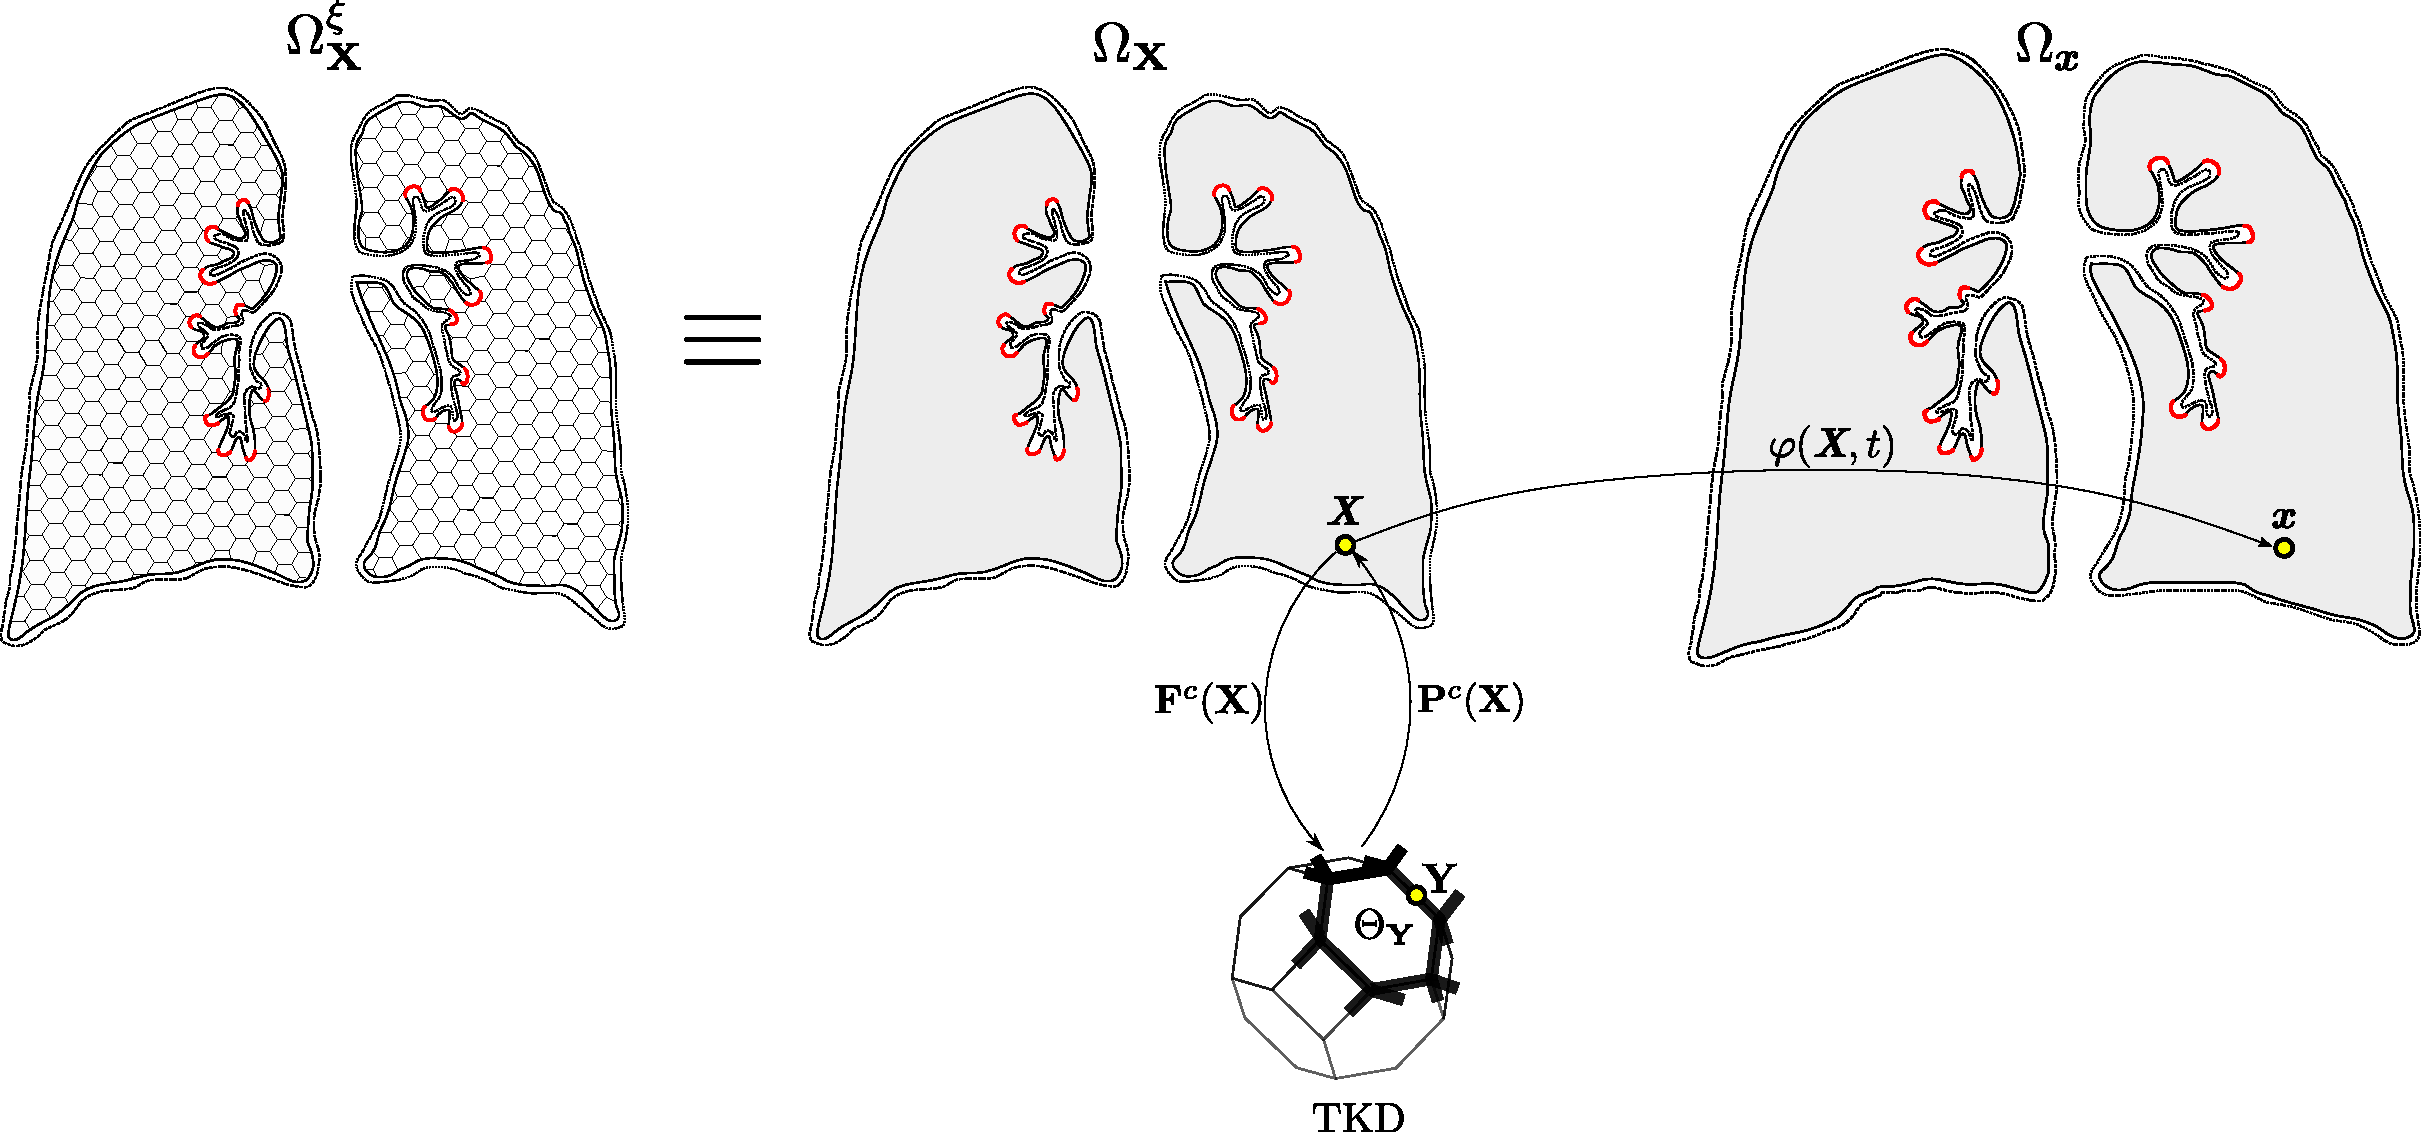
\includegraphics[width=1 \textwidth]{./Figures/domain1.pdf}
     \caption[]{Multiscale modeling approach for lung composite domain $\Omega_X^{\xi}$. Each point $\vec X$ in the coarse scale $\Omega_X$ is informed by a fine-scale TKD micromechanical model with domain $\Theta_Y$. Spatial configuration $\Omega_{x}$ results from applying the $\vec \varphi$ mapping to the coarse-scale reference configuration.
     }
     \label{fig:two-scale-domain}
     \end{center}
\end{figure}
Following a two-scale homogenization approach \cite{BakhvalovPanasenko1989}, we substitute the composite domain as the Cartesian product of a coarse-scale domain and a fine-scale domain, see Figure \ref{fig:two-scale-domain}. Let $\Omega_X$ be the coarse-scale domain in the reference configuration, and $\Theta_Y$ be the locally periodic fine-scale domain with coordinates $\vec X \in \Omega_X$ and $\vec Y \in \Theta_Y$, respectively. We approximate the solid composite domain as the space product $\Omega_{X_S}^{\xi} = \Omega_X \times \Theta_{Y_S}$, and the fluid composite domain as $\Omega_{X_F}^{\xi} = \Omega_X \times \Theta_{Y_F}$, where $\Theta_{Y_S}$ and $\Theta_{Y_S}$ are the solid and fluid phases of the fine-scale domain in the Material configuration and are such that $\Theta_Y = \Theta_{Y_S} \cup \Theta_{Y_F}$ and $\Theta_{Y_S} \cap \Theta_{Y_F} = \emptyset$. Furthermore, $\Theta_{y_S}$ and $\Theta_{y_F}$ represent the spatial configuration for the solid and fluid fine-scale domains, respectively. Let $\hat{\vec X}$ be unit-cell centroid. We note that the fine-scale and coarse-scale coordinates are related through the length scale $\xi$ ($0 < \xi \ll 1$) such that $\vec Y = \frac{1}{\xi} ( \vec X - \hat{\vec X})$. From this relationship, we note that if we express a field in terms of the unit-cell centroid, that is, $f^{\xi}(\vec X)=f (\vec{\hat{X}}, \vec Y)$, then by the chain rule we have \cite{fish2013practical,fish2008mathematical}
\begin{equation}
    \frac{\partial f^{\xi} (\vec X)}{\partial X_j }=\frac{1}{\xi} \frac{\partial f (\vec{\hat{X}}, \vec Y)}{\partial  Y_j}.
    \label{eq:chain-rule}
\end{equation}


\subsection{Homogenization analysis: asymptotic expansion}
We begin our derivation from the classical two-scale asymptotic homogenization theory, where a generic field $h$ is expanded as
\begin{equation}
    h^{\xi}({\vec X}) =h^{(0)}({\vec X}, \vec Y) +\xi h{(1)}({\vec X}, \vec Y) +\xi^2 h^{(2)}({\vec X}, \vec Y) + \mathcal O(\xi^3).
\end{equation} 
For the case of the displacement field, the $\xi^{0}$-term fields are assumed not to depend on $\vec Y$ \cite{fish2013practical}. Based on this, we expand the displacement field as
 \begin{equation}
	\vec u^{\xi} (\vec X) = {\vec u}^{(0)} ({\vec X}) + \xi {\vec u}^{(1)}({\vec X}, \vec Y) + \xi^2 {\vec u}^{(2)} ({\vec X}, \vec Y) + \mathcal O(\xi^3). \label{eq:AsymptoticDisplacement}
\end{equation}
Following the large-strain approach taken in \cite{fish2013practical,fish2008mathematical}, we perform Taylor expansions around the unit-cell centroid $\vec{\hat{X}}$, and rewrite \eqref{eq:AsymptoticDisplacement} as
\begin{equation}
	\vec u^{\xi} (\vec X) = \hat{\vec u}^{(0)} (\hat{\vec X}) + \xi \hat{\vec u}^{(1)}(\hat{\vec X}, \vec Y) + \xi^2 \hat{\vec u}^{(2)} (\hat{\vec X}, \vec Y) + \mathcal O(\xi^3), \label{eq:AsymptoticDisplacement}
\end{equation}
where the components of the displacement fields are
\begin{align}
      \hat{u_i}^{(0)} (\hat{\vec X}) &=u_i^{(0)}(\hat{\vec{X}}),\\
      \hat{u_i}^{(1)} (\hat{\vec X}, \vec Y)&=u_i^{(1)}(\hat{\vec{X}},\vec Y) + \frac{\partial u_i ^{(0)}}{\partial X_j}\bigg|_{\hat{\vec X}} Y_j,\\        \hat{u_i}^{(2)} (\hat{\vec X}, \vec Y) &=  u_i ^{(2)} (\hat{\vec{X}},\vec Y)+ \frac{\partial u_i ^{(1)}}{\partial X_j}\bigg|_{\hat{\vec X}} Y_j+ \frac{1}{2}\frac{\partial^{2} u_i ^{(0)}}{\partial X_j \partial X_k}\bigg|_{\hat{\vec X}}Y_j Y_k,
\end{align}
where in the last expressions we have used Einstein's notation, with repeated indices in one monomial implying summation. For convenience, we define the coarse-scale displacement field by
\begin{equation}
\vec u^c(\vec{\hat X}) := \hat{\vec u}^{(0)}(\vec{\hat X}), 
\end{equation}
and the fine-scale displacement field by
\begin{equation}
    \vec u^f(\hat{\vec X},\vec Y) := \hat{\vec u}^{(1)}(\hat{\vec X}, \vec Y),   
\end{equation}
Applying the derivative rule \eqref{eq:chain-rule} and collecting $\xi$-powers terms, we obtain the coarse-scale and fine-scale deformation gradients \cite{concha2020upscaling}
\begin{align}
	\ten F^c(\hat{\vec X}) &:=  \nabla_X \vec u^c(\hat{\vec X})  + \ten I,\\
	\ten F^f(\hat{\vec X}, \vec Y) &:=  \nabla_X \vec u^f(\hat{\vec X}, \vec Y) + \ten I,
\end{align}
respectively. Further, we expand the solid First Piola-Kirchhoff stress field as
\begin{equation}
\ten{P}_S^{\xi}=\hat{\ten{P}}_S^{(0)}(\hat{\vec X}, \vec Y)+\xi \hat{\ten{P}}_S^{(1)}(\hat{\vec X}, \vec Y)+O(\xi^2). \label{eqn:PSexpansion}
\end{equation}  
For convenience, we define the fine-scale First Piola-Kirchhoff stress tensor as $	\ten P_S^{f}:= \ten P_S^{(0)}$ \cite{fish2013practical}. Then, substituting \eqref{eqn:PSexpansion} into \eqref{eqn:SolidEquilibrium}, applying the derivative rule \eqref{eq:chain-rule}, and matching $\xi$-powers terms we get
\begin{eqnarray}
	 \nabla_Y \cdot {\ten P_S^{f}(\hat{\vec X}, \vec Y)} &=& \vec 0 \quad \mbox{in } \Omega_X \times \Theta_{Y_S}, \label{eq:FineEquilibrium} \\
	\nabla_X \cdot \ten P_S^{f} (\hat{\vec X}, \vec Y) + \nabla_Y \cdot \ten P_S^{(1)}(\hat{\vec X}, \vec Y) &=& \vec 0 \quad \mbox{in } \Omega_X \times\Theta_{Y_S}, \label{eq:CoarseEquilibrium}
\end{eqnarray}
and we note that \eqref{eq:FineEquilibrium} defines the {\it governing equation for the fine-scale solid problem}, see also \cite{concha2020upscaling}.\\ 
For the formulation of the fluid problem, we expand the composite fluid pressure and velocity fields as 
\begin{align}
	p^{\xi} (\vec x) &= \hat{p}^{(0)} (\hat{\vec x}, \vec y) + \xi \hat{p}^{(1)}(\hat{\vec x}, \vec y) + \mathcal O(\xi^2), \label{eq:AsymptoticPressure} \\
	\vec v_i^{\xi} (\vec x) &= \hat{\vec v_i}^{(0)} (\hat{\vec x}, \vec y) + \xi \hat{\vec v_i}^{(1)}(\hat{\vec x}, \vec y) + \mathcal O(\xi^2),  \label{eq:AsymptoticVelocity}
\end{align}
respectively, where
\begin{align}
	\hat p^{(0)} (\hat{\vec X}, \vec Y) = 	p^{(0)} (\hat{\vec X}, \vec Y), \quad 	\hat p^{(1)} (\hat{\vec X}, \vec Y) =  \left. \pd{p^{(0)}}{X_j}   \right|_{\vec{\hat X}} Y_j + p^{(1)}(\vec {\hat X}, \vec Y),\\
	\hat v_i^{(0)} (\hat{\vec X}, \vec Y) = 	v_i^{(0)} ( \hat{\vec X}, \vec Y), \quad 	\hat v_i^{(1)} (\hat{\vec X}, \vec Y) =  \left. \pd{v_i^{(0)}}{X_j}   \right|_{\vec{\hat X}} Y_j + v_i^{(1)}(\vec {\hat X}, \vec Y). 
\end{align}
Using arguments analogous to those considered in for the solid problem, it follows from the multiscale expansion of equation \eqref{eqn:FluidEquilibrium} that
\begin{eqnarray}
	\nabla_y \cdot \ten{\sigma}_F^{(0)}(\hat{\vec x}, \vec y) &=& \vec 0 \quad \mbox{in $\Omega_x \times \Theta_{y_F }$}  \label{eqn:EqfluidExp1},  \\
	\nabla_x \cdot \ten{\sigma}_F^{(0)} (\hat{\vec x}, \vec y)  + \nabla_y \cdot \ten{\sigma}_F^{(1)}(\hat{\vec x}, \vec y)&=& \vec 0    \label{eqn:EqfluidExp2} \quad \mbox{in $\Omega_x \times\Theta_{y_F}$},
\end{eqnarray}
where we had expanded the fluid Cauchy stress tensor as 
\begin{equation}
\ten{\sigma}_F^{\xi}=\hat{\ten{\sigma}}_F^{(0)}(\hat{\vec x}, \vec y)+\xi \hat{\ten{\sigma}}_F^{(1)}(\hat{\vec x}, \vec y)+O(\xi^2). \label{eqn:sigmaFexpansion}
\end{equation}
Further, expanding equation \eqref{eqn:AdimensionalFluidStress} and matching $\xi$-powers terms  results in
\begin{eqnarray}
	\ten \sigma_F^{(0)} (\hat{\vec x}, \vec y) &=& -p^{(0)} (\hat{\vec x}, \vec y) \ten I	\quad \mbox{in } \Omega_x \times \Theta_{y_F} \label{zero_stress_fluid_fine}, \\
	\ten \sigma_F^{(1)}(\hat{\vec x}, \vec y) &=& -p^{(1)} (\hat{\vec x}, \vec y) \ten I + \mu \left(  \nabla_y \vec v^{(0)}(\hat{\vec x}, \vec y)  + (\nabla_y \vec v^{(0)}(\hat{\vec x}, \vec y) )^T \right) \quad \mbox{in } \Omega_x \times \Theta_{y_F},
\end{eqnarray}
and substituting these expressions into \eqref{eqn:EqfluidExp1} and \eqref{eqn:EqfluidExp2} we obtain
\begin{eqnarray}
	-\nabla_y p^{(0)}(\hat{\vec x}, \vec y) &=& \vec 0 \quad \mbox{in } \Omega_x \times\Theta_{y_F}, \label{eq:coarse_scale_pressure}\\
	- \nabla_y p^{(1)}(\hat{\vec x}, \vec y) +  {\mu} \nabla_y \cdot \nabla_y \vec v^{(0)}(\hat{\vec x}, \vec y)   - \nabla_x p^{(0)}(\hat{\vec x}, \vec y) & =& \vec 0 \quad \mbox{in } \Omega_x \times\Theta_{y_F}. \label{eq:fine_scale_fluid_equilibrium}
\end{eqnarray}
From \eqref{eq:coarse_scale_pressure} we conclude that $p^{(0)} = p^{(0)}(\vec{\hat x})$. Then, we  define the coarse-scale pressure and fine-scale pressure  as $p^{c}(\hat{\vec x}):=  p^{(0)}(\vec{\hat x})$ and $p^{f} (\hat{\vec x}, \vec y):= p^{(1)} (\hat{\vec x}, \vec y)$, respectively.\\ 
Asymptotic expansion and power matching on the fluid mass conservation equation \eqref{eqn:MassEquilibrium} yields
\begin{eqnarray}
	\nabla_y \cdot \vec v^{(0)}(\hat{\vec x}, \vec y)  &=& 0 \quad \mbox{in } \Omega_x \times\Theta_{y_F}, \label{eq:fine_scale_mass_conservation} \\
	 \nabla_x \cdot  \vec v^{(0)}(\hat{\vec x}, \vec y) +  \nabla_y \cdot \vec v^{(1)}(\hat{\vec x}, \vec y) &=& 0 \quad \mbox{in } \Omega_x \times\Theta_{y_F} ,\label{eq:coarse_scale_mass_conservation}
\end{eqnarray}
and we define the fine-scale velocity as $	v^{f} (\hat{\vec x}, \vec y) := v^{(0)} (\hat{\vec x}, \vec y)$. 

Finally, we apply asymptotic expansion and match $\xi$-power terms for the stress compatibility given by \eqref{eqn:compatibilty_stress} to obtain
\begin{align}
	 \ten P_S^{(0)} \vec N&= \left (\ten{\sigma}_F^{(0)} \    \ten H^{(0)} \right) \circ \vec \varphi(\vec{\hat X}, \vec Y) \ \vec N \quad \mbox{on $\partial \Theta_{Y_{FS}}$,}\\
	 \ten P_S^{(1)} \vec N&= \left(\ten{ \sigma}_F^{(0)}  \ \ten H^{{(1)}} + 
	\ten{{ \sigma}}_F^{(1)}  \ \ten H^{{(0)}} \right) \circ \vec \varphi(\vec{\hat X}, \vec Y) \  \vec N \quad  \mbox{on $\partial \Theta_{Y_{FS}}$},
\end{align}
and, proceeding analogously, from the velocity compatibility \eqref{eqn:compatibilty_vel} we obtain that 
\begin{align}
	\pd{\vec u^{(0)} (\vec {\hat X}) }{t} &= \vec v^{(0)} \circ \vec \varphi (\vec {\hat X}, \vec Y) \qquad &\mbox{on $\partial \Theta_{Y_{FS}}$,} \\
	\pd{\vec u^{(1)} (\vec{\hat X}, \vec Y) }{t} &= \vec v^{(1)} \circ \vec \varphi (\vec {\hat X}, \vec Y) \qquad &\mbox{on $\partial \Theta_{Y_{FS}}$} .
\end{align}


\subsection{Upscaling relations and coarse-scale governing problems}
To establish a relation between fine and coarse scale problems, we consider \eqref{eq:CoarseEquilibrium}. Integrating in the solid fine-scale domain, using the interface boundary conditions, and assuming periodicity in the purely solid and purely fluid boundaries yields
\begin{equation}
	\int_{\Theta_{Y_S}} \nabla_X \cdot \ten P_S^{f} \ d \Theta_{Y_S} - 
\int_{\Theta_{Y_{F}}} \nabla_Y \cdot \ten P_F^{(1)}  \ d \Theta_{Y_{F}}  = \vec 0.  \label{solidcoarse1}
\end{equation}
Transforming \eqref{eqn:EqfluidExp2} to the Material configuration and using \eqref{zero_stress_fluid_fine} for the leading-order fluid stress tensor, we obtain
\begin{equation}
	\nabla_Y \cdot \ten P_F^{(1)} =  \nabla_X \cdot ( P^c \ten H^{(0)} ),
\end{equation}	
where $P^c= p^{c} \circ \vec{\varphi}$. 
 Inserting this expression into equation \eqref{solidcoarse1}, taking the average of each term, and noting that $P^c$ does not depend on the fine scale, the coarse-scale linear momentum conservation reads
\begin{equation}
\nabla_X \cdot   (\ten{P}_S^{c} - P^c \ten H^{c} )
 = \vec 0 \quad \text{in } \Omega_{X}, \label{eqn:lmc}
\end{equation}
where
\begin{equation}
    \ten P_S^{c}= \frac{1}{\| \Theta_{Y} \|} \int_{\Theta_{Y_S}}  \ten P_S^{f} \ d \Theta_{Y_S},\label{eq:upscale-solid}
\end{equation}

\begin{equation}
    \ten H^{c}=   \frac{1}{\| \Theta_{Y} \|}
\int_{\Theta_{Y_{F}}}    \ten H^{(0)}     \ d \Theta_{Y_{F}}.
\label{eq:fluid-contribution}
\end{equation}
In particular, we note that \eqref{eq:upscale-solid} provides an upscaling relation for the solid response. Following a standard poroelasticity formulation, we will assume the fluid contribution to the stress tensor defined in \eqref{eq:fluid-contribution} to be an isotropic tensor in the current configuration (Terzaghi effective stress principle), such that it represents the hydrostatic effect of pore pressure, i.e.,
\begin{equation}
    \ten H^{(0)} = J^C \left(\ten{F^c}\right)^{-T}.
\end{equation}
Based on this consideration, the coarse-scale linear-momentum conservation equation takes the form
\begin{equation}
\nabla_X \cdot \ten P_S^{eff}
  = \vec 0 \quad \text{in } \Omega_{X},
\end{equation}
where the coarse-scale effective stress tensor is defined by
\begin{equation}
\ten P_S^{eff} = \ten{P}_S^{c} - J^c P^c \left(\ten{F^c}\right)^{-T}. \label{eqn:effectiveStress}
\end{equation}

To derive the coarse-scale formulation for the fluid mass conservation, we integrate equation \eqref{eq:coarse_scale_mass_conservation} and use the divergence theorem in its second term to write
\begin{equation}
\int_{\Theta_{y_F}}\nabla_x \cdot \vec v^{f} \ d \Theta_{y_F} + 
 \int_{\partial \Theta_{y_F}}  \vec v^{(1)} \cdot \vec n   \ d \partial  \Theta_{y_F} + 
 \int_{\partial \Theta_{y_{FS}}}  \vec v^{(1)} \cdot \vec n   \ d \partial  \Theta_{y_{FS}} = 0.
\end{equation}
Using periodicity conditions and assuming that the velocity of the solid is negligible compared to that of the fluid, we obtain
\begin{equation}
	\nabla_x \cdot\int_{\Theta_{y_F}} \vec v^{f} \ d  \Theta_{y_F} = 0.
\end{equation}
Following \cite{fish2013practical}, we introduce the ansatz $\vec v^{f} = \ten w  \nabla_x p^c$, with $\vec w$ an auxiliary field, and take the average in the unit cell to arrive to
\begin{equation}
	\nabla_x \cdot \left( \ten k  \nabla_x p^{c} \right)  = 0, 
\end{equation}
where
\begin{equation}
	\ten k = \frac{1}{\| \Theta_{y} \|}  \int_{\Theta_{y_F}} \ten w \ d \Theta_{y_F}. 
	\label{eq:k-tensor}
\end{equation} 
Finally, performing a pull-back operation on \eqref{eq:k-tensor}, 
we arrive at the Material coarse-scale mass-balance equation
\begin{align}
	\nabla_X \cdot \left(  J^c \ten F^{c^{-1}} \ten K \ten F^{c^{-T}} \nabla_X P^c       \right)  = 0 \label{eqn:MassConservation_quasi}
	\quad \mbox{ in $\Omega_X$},
\end{align}
where $\ten K = \ten k \circ \vec \varphi$ the permeability tensor. We note that the computation of this tensor requires the solution of the auxiliary function $\vec w$ on a unit-cell problem for the fluid phase. However, for simplicity, we assume a constant and isotropic permeability such that $\ten K=K \ten I$, with $K=10^{4}$ mm$^2$/kPa$\cdot$s \cite{berger2016poroelastic,avileshurtado2022whole}.\\
At this point, we note that \eqref{eqn:MassConservation_quasi} corresponds to a steady-state problem from mass conservation. To consider the transient regime of airflow in the lungs, we add to this balance statement the variation of fluid mass measured in terms of a  porosity field to arrive to
\begin{equation}
\frac{\partial \Phi}{\partial t} +\nabla_X \cdot \vec{Q}^c = 0  \quad \mbox{ in $\Omega_X \times (0,T]$},	\label{eqn:MassConservation_temporal}
\end{equation}
where 
\begin{equation}
 \vec{Q}^c=    J^c \ten F^{c^{-1}} \ten K \ten F^{c^{-T}} \nabla_X P^c, \label{eq:mat-flux}   
\end{equation}
is the Material flux field, and $\Phi$ the Material porosity field, that for a media with incompressible solid and fluid phases can be further computed as
\begin{equation}
    \Phi=J^c+\Phi_0-1
\end{equation}
where  $\Phi_0$ is the initial Material porosity \cite{coussy2004poromechanics,macminn2016large}.

\subsection{Weak formulation of the multi-scale fluid-solid problem}
Collecting the coarse-scale governing equations and upscaling relations derived in previous sections, we state the strong formulation of the multiscale fluid-solid interaction problem as follows: Find $\var \varphi^c:\Omega_X \times \R \to \R^3$ and $P^c:\Omega_X \times \R \to \R$ such that
\begin{eqnarray}
	 \nabla_X \cdot  	\ten P_S^{eff} &=\vec 0 &\quad \mbox{ in $\Omega_X \times (0,T]$ }  \label{eqn:LinearMomentumConservationFinal} \\
	 \dfrac{\partial \Phi}{\partial t} +\nabla_X \cdot \vec{Q}^c &=0 &\quad \mbox{ in $\Omega_X \times (0,T]$ }  \label{eqn:MassConservationFinal}   \\
	 \vec \varphi^c &= {\vec{ \varphi}_0^c} &\quad \mbox{ in $\partial \Omega_X$}  \\
	 P^c &=  P_0^c &\quad \mbox{ on $\partial \Omega_X$} \\
	 \vec \varphi^c &= {\vec{\bar \varphi}^c} &\quad \mbox{ on $\partial \Omega_X^{\varphi}$} \times (0,T] \\
	\ten P_S^{eff}  \cdot \vec N &= \vec{\bar T}^{c} &\quad \mbox{ on $\partial \Omega_X^T$} \times (0,T] \label{eqn:bc_traction}\\
	 P^c &= \bar P^c &\quad \mbox{ on $\partial \Omega_X^P$}\times (0,T] \\
	 \vec{Q}^c \cdot \vec N &= {\bar Q}^c &\quad \mbox{ on $\partial \Omega_X^Q$} \times (0,T] \label{eqn:bc_flux},
\end{eqnarray}
where $\ten P^{eff}$ and $\ten Q^c$ are defined by Eqns. \eqref{eqn:effectiveStress} and \eqref{eq:mat-flux}, respectively.\\

For the construction of a non-linear finite-element solution to this problem, we seek the associated weak formulation. To this end, we define the following trial and test function spaces 
\begin{align}
&\mathcal{S}_{\varphi^c}:= \{ \vec{\varphi}^c:{\vec{\varphi}^c} \in  H^1(\Omega_0,\R^3) ; \   {\vec{\varphi}}^c =\bar{{\vec{\varphi}}}^c \ ~ \text{on}  ~ \partial \Omega_X^{\varphi} \},\\
&\mathcal{V}_{\varphi^c} := \{  \vec{\eta}^c:\vec{\eta}^c \in  H^1(\Omega_0,\R^3) ; \   {\vec{\eta}}^c =\vec{0} \  ~ \text{on}  ~ \partial \Omega_X^{\varphi} \}, \\
&\mathcal{S}_{P^c}:= \{ P^c \in  H^1(\Omega_0,\R) ; \   P^c=\bar{P} ^c ~ \text{on}  ~\partial \Omega_X^{P} \}, \\
&\mathcal{V}_{P^c} := \{ q^c \in  H^1(\Omega_0,\R) ; \   q^c=0  ~ \text{on}  ~ \partial \Omega_X^{P} \}.
\end{align}
To derive the weak form associated to the linear momentum balance equation, we multiply \eqref{eqn:LinearMomentumConservationFinal} by $\vec{\eta}^c \in \mathcal{V}_{\varphi^c}$,  apply integration by parts,  use the boundary condition \eqref{eqn:bc_traction} and expand the expression for $\ten P^{eff}$ to get the subproblem: Find $\vec{\varphi}^c \in \mathcal{S}_{\varphi^c}$ and $P^c \in \mathcal{S}_{P^c}$ such that
\begin{equation}
	\int_{\Omega_X} \ten P_S^{c} :  \nabla_X \vec{\eta}^c  \ d \Omega_X 
	- \int_{\Omega_X}\left( J^c P^c \left(\ten{F^c}\right)^{-T} \right): \nabla_X \vec{\eta}^c  \ d \Omega_X  
-
	\int_{\partial \Omega_X}  \vec T_S^c \cdot \vec{\eta}^c  \ d \partial \Omega_X=0,
	\label{eq:solid-residual}
\end{equation}
for any $\vec \eta^c \in \mathcal{V}_{\varphi^c}$. For the case of the fluid coarse-scale problem, we multiply \eqref{eqn:MassConservationFinal} by $q^c \in \mathcal{V}_{P^c}$, use the integration by parts theorem, and consider the boundary condition \eqref{eqn:bc_flux} to arrive at the weak equation
\begin{equation}
	\int_{\Omega_X}\frac{\partial \Phi}{\partial t} q  \ d \Omega_X   - \int_{\Omega_X}  \vec Q^c  \cdot \nabla_X \  q \ d \Omega_X +
	\int_{\partial \Omega_X} \bar{Q}^c q\ d \partial \Omega_X =0,
		\label{eq:fluid-residual}
\end{equation}  
for any $q^c \in \mathcal{V}_{P^c}$.\\

The weak-form residuals \eqref{eq:solid-residual} and \eqref{eq:fluid-residual} were discretized in time using a backward-Euler integration scheme. The space fields were discretized using a standard Galerkin finite-element (FE) formulation to obtain a dynamic multi-field FE problem \cite{HurtadoCastroMadrid2017,HurtadoZavala2021}. To solve this FE problem numerically, we developed an enhanced version of the FEniCS library \cite{Fenics2012}, where functions solving the fine-scale problem were coupled to non-linear FE solvers. The element multi-field formulation considered a Taylor-Hood (P2-P1) interpolation scheme.

%\rev{In the next, we will see that, given the structure of the TKD model, it is more convenient to formulate the weak formulation with the symmetrical stress tensor $\ten S_S^c$ instead of $\ten P_S^c$. Thus, noting that $\ten P_S^{c}=\ten{F^c}\ten S_S^c$ and using symmetry properties we get}
%\begin{equation}
%	\int_{\Omega_X}   \ten S_S^{c} : D \ten E^c  \ d \Omega_X 
%	- \int_{\Omega_X}   \left( J^c P^c \left(\ten{F^c}\right)^{-T} \right):\nabla_X\vec{\eta}^c \ d \Omega_X  
%-
%	\int_{\partial \Omega_X} \vec T_S^c \cdot  \vec{\eta}^c  \ d \partial \Omega_X=0
%\end{equation}
%with 
%\begin{equation}
%    D \ten E^c=\frac{1}{2} \Big( (\ten{F^c})^T \nabla_X \vec{\eta}^c + ( \nabla_X \vec{\eta}^c )^T  \ten{F^c} \Big)
%\end{equation}


\subsection{Fine-scale problem: The tetrakaidecahedron (TKD) model}\label{sec:TKDmodel}

To inform the coarse-scale constitutive relation defined by \eqref{eq:upscale-solid}, the fine-scale solid problem needs to be solved first. In this work, for the fine-scale problem, we consider the tetrakaidecahedron (TKD) model proposed by \citet{concha2020upscaling}, which has been developed for alveolar microstructures. In the following, we summarize the main aspects of this micromechanical model.\\  
The TKD geometry can be observed in Figure \ref{fig:two-scale-domain}. Based on symmetry considerations \cite{ConchaEtal2018}, we consider a subregion of it, denoted as TKDr, which is representative of the entire TKD, and can also represent an infinitely periodic network of TKD elements. The TKDr is formed by strut elements that can only deform axially and whose strain energy density function is given by the NeoHookean incompressible energy density
\begin{eqnarray}
	W(\ten F)  &=& \frac{\mu}{2}\left\{\mbox{tr}({\ten F}^T \ten F) - 3\right\} - w(\mbox{det} \ten F - 1),
	\label{eq:conslaw}
\end{eqnarray}
where $\mu$ is the Lam\'e parameter and $w$ is a Lagrange multiplier used to enforce the incompressibility constraint 
\begin{equation}
	\det \ten F = 1 \quad \text{in } \Theta_{Y_S}.
	\label{eq:incomp} 
\end{equation}
To solve the solid fine-scale problem, we reformulate the associated boundary value problem as a saddle-point variational problem which can be written as
\begin{align}
	\min \limits_{\substack{\vec u \in \vec u_{adm}}} \ 
	\max \limits_{w \in L^2(\Theta_{Y_S})}  
	\int_{\Theta_{Y_S}} \left[ 
	\frac{\mu}{2}\left\{ \tr[ {(\ten I + \nabla_o \vec u^f)}^T (\ten I + \nabla_o \vec u^f) ] -3 \right\}
	- w(\det (\ten I + \nabla_o \vec u^f) -1) \right] \ d\Theta_{Y_S}	 
	- \notag \\ 
	\int_{\partial \Theta_{Y_{SF}}} \left[ \vec u^f \cdot P_{alv}^c \det(\ten I + \nabla_o \vec u^f) (\ten I + \nabla_o \vec u^f)^{-T} \vec N  \right] \ dS,
	\label{eq:varprin}
\end{align}
where $\nabla_0$  is the gradient operator concerning the Material configuration. To solve this variational problem, we represent the TKDr by a truss structure with a square cross-section and elements connected at joints in the intersections. We denote by $\vec Q_e$ and $\vec q_e$ the difference between end-node coordinates in the reference and current configuration for the $e-$th element, respectively. Let $h_o$ and $h_e$ be the reference and current cross-section dimension of an element, respectively, and $L_{eo}=||\vec Q_e||$ the reference length of the element. From these definitions, we define the axial and transverse stretch ratios of the $e$-th element by
\begin{equation}
	\lambda_e := \frac{\| \vec q_e \| }{L_{eo}} \qquad e=1,18,
\end{equation}
\begin{equation}
	\lambda_e^T := \frac{h_e}{h_o} \qquad e=1,18,
\end{equation}
respectively. Using these definitions, we can express the deformation gradient tensor of the $e-$th element in local coordinates as
\begin{equation}
	\ten F_e = 
	\begin{bmatrix}
		\lambda_e		&	0	&	0\\
		0	&	\lambda_e^T	&	0\\
		0	&	0	&	\lambda_e^T
	\end{bmatrix}.
	\label{eq:Ftruss}
\end{equation}
The potential energy of the TDKr structure considers the contribution of each element's deformation (axial) energy, the work done by alveolar pressure acting on the surface of each element, and a rotational energy term for each joint of the structure. Then, the total potential energy can be written as
\begin{equation}
	\Pi = \sum_{e=1}^{18} \Pi_e^{\rm axial} (\vec q_e, \lambda^T_e, w_e ) -  \sum_{e=1}^{18} \Pi^{\rm pressure}_{e} (\lambda^T_e; p^c) + \sum_{j \in \mathcal J} \Pi^{\rm rotational}_{j}(\vec q_{j1}, \vec q_{j2})
\end{equation}
with the axial, pressure and rotational energies terms computed as \cite{concha2020upscaling}
\begin{align}
	\Pi^{\rm axial}_e(\vec q_e, \lambda_e^T, w_e) &  = A_{o} L_{eo} \left\{ \frac{\mu}{2} (\lambda_e^2 + 2{\lambda_e^T}^2 - 3) - w_e(\lambda_e (\lambda_e^T)^2 - 1) \right\}, \\
	\Pi^{\rm pressure}_e( \lambda_e^T; p_{alv}^c) &= - 2 A_o L_{eo} \ P_{alv}^c  \lambda_e (\lambda_e^{T^2} - \lambda_e^T),\\
\Pi^{\rm rotational}_{j}(\vec q_{j1},\vec q_{j2}) &= \frac{1}{2} k_{\theta} \, \left\{  \frac{\vec q_{j1} \cdot \vec q_{j2}}{\| \vec q_{j1} \| \, \| \vec q_{j2} \|} - \frac{\vec Q_{j1} \cdot \vec Q_{j2}}{\| \vec Q_{j1} \| \, \| \vec Q_{j2} \|} \right\}^2 ,	
\end{align}
respectively. In the previous equations $w_e$ is the Lagrange parameter for the $e$-th element, $k_{\theta}$ is the rotational stiffness expressed as
\begin{equation}
	k_{\theta} = \alpha \frac{EI}{2 \delta},
\end{equation}
with $\alpha$ a rotational parameter to be fitted, $E = 3\mu$ is the alveolar-wall elastic modulus, $I$ is the flexural inertia moment of a square cross-section, $\delta$ is the initial strut half-length, and $A_0$ the  reference cross-
sectional area, which can be computed as \cite{ConchaEtal2018}
\begin{equation}
A_o = \frac{32\sqrt{2} (1-f_o)\delta^2}{12-9d},
\end{equation}
where $d$ is an overlapping parameter, to be calibrated, and
\begin{equation}
	f_0 := 1 - \frac{|\Theta_{Y_S}|}{|\Theta_Y|},
\end{equation}
is the initial reference porosity of the lung microstructure. \\

The TKD model assumes as an input a principal deformation state. To account for this assumption, we apply the polar decomposition theorem on the coarse-scale deformation-gradient tensor, i.e. $\ten F^c = \ten R^c \ten U^c$, and consider the stretch tensor to take the form
\begin{equation}
	\ten U^c = 
	\begin{bmatrix}
		\lambda_1^c	&	0	&	0\\
		0	&	\lambda_2^c	&	0\\
		0	&	0	&	\lambda_3^c
	\end{bmatrix}
	\label{eq:Fc}
\end{equation}
where $\lambda_1^c, \lambda_2^c, \lambda_3^c$ are the coarse-scale principal stretches. We further consider a reduced set of degrees of freedom $\vec r$ for the TKDr structure, which can be related to the remaining degrees of freedom from symmetry considerations. Then, the TKD nodal displacements can be expressed as
\begin{equation}
	\vec u_i = \vec u_i(\vec r; \ten U^c) \quad \forall i=1,18
\end{equation}
Letting $\mat w = [w_1, \ldots, w_{18}]^T$ and $\mat l = [\lambda_1^T,\ldots,\lambda_{18}^T]$, we rewrite the variational principle \eqref{eq:varprin} as the optimization problem
\begin{equation}
	\min \limits_{\mat r \in \R^3, \; \mat l \in \R^{18}} \quad \max \limits_{\mat w \in \R^{18}} \quad \Pi (\mat r, \mat l, \mat w; \ten U^c, P_{alv}^c)
\label{eqn:FullMinimizationProblem}
\end{equation}
where the strut variables $\lambda^T_e, w_e$ can be locally solved such that $\mat l = \mat l (\mat r;\ten U^c)$ and  $\mat w = \mat w(\mat r; \ten F^c, P_{alv}^c)$. Thus, the minimization problem reduces to
\begin{equation}
	\min \limits_{\mat r \in \R^{3}} \quad \Pi^{\rm eff} (\mat r; \ten U^c, p_{alv}^c)
	\label{eq:effmin} = \Pi^{\rm eff} (\mat r^*; \ten U^c, P_{alv}^c),
 \label{eq:eff-min}
\end{equation}
where $\vec r^{*}$ corresponds to the solution of the effective minimization problem. Finally, to compute the stress state, we use Hill's Lemma for large deformations, so
\begin{equation}
	\ten P^c =\frac{1}{V_0} \frac{D \Pi^{eff}}{D \ten U^c} (\mat r; \ten U^c, P_{alv}^c),
\end{equation}
 or equivalently,
\begin{equation}
	\hat{\ten P}^c = \frac{1}{V_0} \left[ \pd{\Pi^{eff} (\mat r^{*}; \ten U^c, p_{alv}^c) }{\vec r} : \pd{\vec r}{\ten U^c} + \pd{\Pi^{eff} (\mat r^{*}; \ten U^c, P_{alv}^c) }{\ten U^c} \right]
\end{equation}
where  $V_0$ is the initial TKDr volume. Since $\pd{\Pi}{\vec r}$ is evaluated at the solution of the minimization problem \eqref{eq:eff-min}, and the coarse-scale principal stress tensor takes the form
\begin{equation}
	\hat{\ten P}^c = \frac{1}{V_0} \pd{\Pi^{eff} (\mat r^{*}; \ten U^c, P_{alv}^c) }{\ten U^c}. \label{eqn:Hill_P}
\end{equation}
As a last step, we use the principal stresses in \eqref{eqn:Hill_P} to construct the coarse-scale Piola-Kirchhoff tensor as
\begin{equation}
    \ten P^c = \sum_{\alpha=1}^3 \hat{P}^c_{\alpha} \hat{\vec n}_{\alpha} \otimes \hat{\vec N}_{\alpha},
\end{equation}
where $\{ \hat{\vec N}_{\alpha} \}_{\alpha=1,2,3}$ and $\{ \hat{\vec n}_{\alpha} \}_{\alpha=1,2,3}$ are the Material and spatial principal directions associated to $\ten F^c$.





%%%%%%%%%%%%%%%%%%%%%%%%%%%% RESULTS %%%%%%%%%%%%%%%%%%%%%%%%%%%%%%%%%%
\section{Numerical simulations} \label{sec:numerical-simulations}

\subsection{Model setup}
To demonstrate the capabilities of the proposed multiscale framework, we constructed a non-linear finite-element lung model using an anatomical geometry, see Figure \ref{fig:lung-mesh}. We obtained the lung domain by segmenting a thoracic computed-tomography image acquired for a normal subject, see \cite{HurtadoEtal2016,HurtadoEtal2017} for more details. Based on the lung domain, we generated a tetrahedral lung mesh using the CGAL library \cite{cgal}. The mechanical interaction of the lung tissue with the rib cage and the mediastinum was modeled through continuous elastic elements represented by a Robin boundary condition of the form
	 \begin{equation}
	     \bar{\vec{T}}^c(\vec X)={K}_\text{s} \left\{\vec{\varphi(\vec X) -X} \right\} \qquad \text{ on } \partial \Omega_X,
	 \end{equation}
which applies to the entire lung boundary. In all simulations, we considered ${K}_\text{s}=80\cdot 10^{–3}$ kPa/mm, which has shown to deliver a chest-wall compliance value that falls within the range observed in normal subjects \cite{avileshurtado2022whole}. For the prescription of boundary conditions for the gas flow equation, we partitioned the lung boundary into the surface occupied by the visceral pleura and the surface that delimited the airway boundary, taken as the bronchi cross sections \cite{avileshurtado2022whole}. A no-flux Neumann boundary condition was prescribed on the visceral pleura surface in all cases. The choice of boundary condition on the airway boundaries depended on the ventilation mode studied, as we detail below.\\

\begin{figure}[h!]
    \begin{center}
    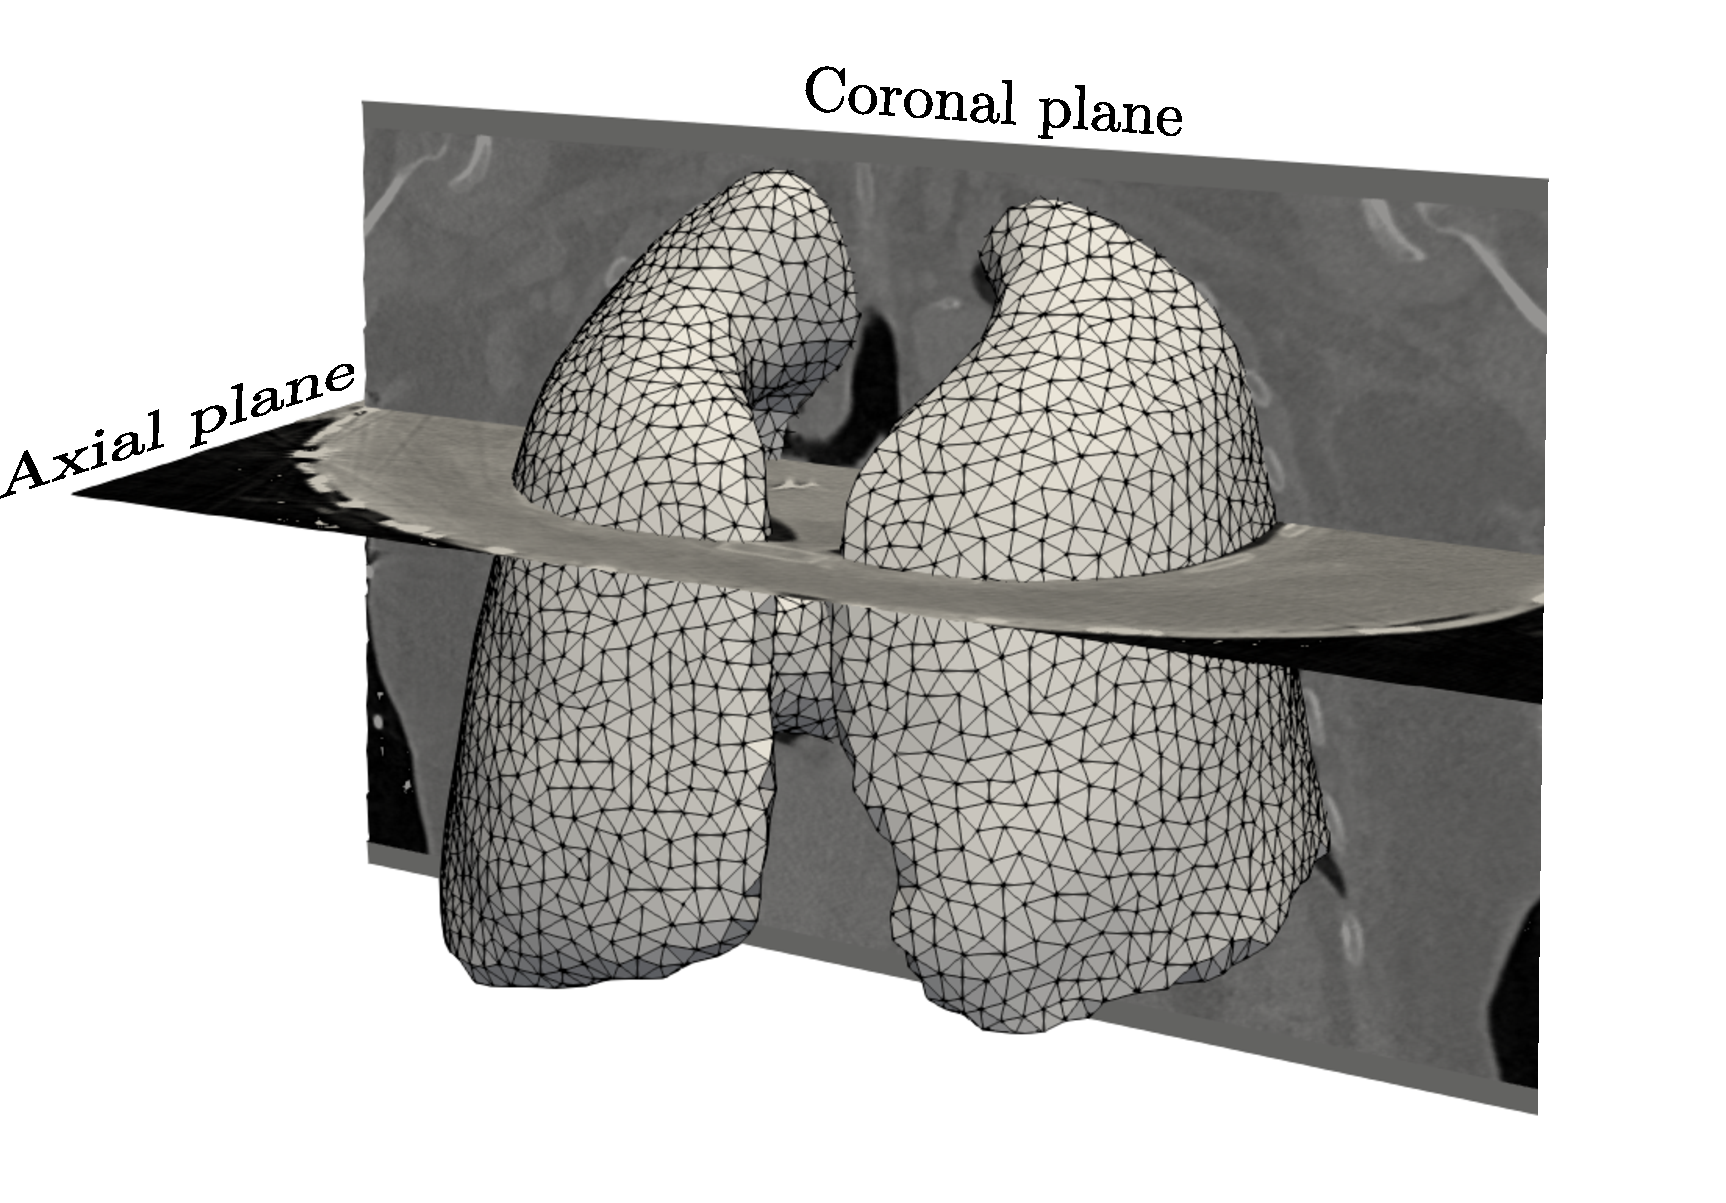
\includegraphics[width=0.7 \textwidth]{./Figures/mesh2.pdf}
    \caption[]{Anatomical finite-element mesh constructed for the lung simulations. The lung domain was determined from computed-tomography images of a normal human volunteer. Axial and coronal planes are shown for further reference.}
    \label{fig:lung-mesh}
    \end{center}
\end{figure}

To model the interaction between the lung and the air supplied by an external mechanical ventilator, we restricted airflow to take place only on the airway boundaries. Due to their relevance in the clinical setting, two modes of mechanical ventilation were considered in this study, we refer the reader to \cite{avileshurtado2022whole} for further details. In the pressure-controlled ventilation (PCV) mode, the mechanical ventilator imposes the airway-pressure signal, represented by a function denoted by $\bar{P}(t)$. At the beginning of inspiration, the pressure rapidly rises until it reaches a peak value of 5 cm H$_2$0 in 0.1 seconds, a pressure that is then maintained constant until the end of the inspiration phase, whose duration in total is 1 second. Then, this pressure is suddenly reduced to zero and maintained at this value for the next 2 seconds during the expiratory phase. In our simulations, this airway pressure signal was prescribed on the airway boundary. Once the simulation was carried out, the lung volume $\text{V}(t)$ and airway flow $\dot{\rm{V}}(t)$ signals were computed during a post-processing step as

\begin{equation}
    \text{V}(t):= \int_{\Omega_0} J \, d\Omega_0 - \int_{\Omega_0}  \, d\Omega_0, \label{eq:Vsim}
\end{equation}
and
\begin{equation}
    \dot{\rm{V}}(t):= \int_{\Gamma_\text{aw}} \vec Q \cdot \vec N \, d \Gamma_\text{aw},
    \label{eq:Qsim}
\end{equation}
where $\Gamma_\text{aw}$ represents the airway boundary.\\

The volume-controlled ventilation (VCV) mode considers the case where the mechanical ventilator prescribes the airway flow so as to achieve a predefined level of maximum lung volume during each cycle. To this end, the airway flow $\bar{Q}(t)$ was set to a constant level for 1 second, followed by an inspiratory pause of 0.25 seconds of zero flow ($\bar{Q}(t)=0$). After this pause, the boundary condition on the airway boundary changed to prescribed pressure, with $\bar{P}(t)=0$ to allow for a passive expiration process. Using the results from the inspiratory phase, we computed the airway pressure $\text{P}_\text{aw}(t)$ and lung volume $\text{V}(t)$ signals as
\begin{equation}
\text{P}_\text{aw}(t):=\frac{1}{\text{A}_\text{aw}}\int_{\Gamma_\text{aw}} {P}_{alv}(\vec{X,t}) \  d\Gamma_\text{aw}, \label{paw_avg}
\end{equation}
\begin{equation}
    \text{V}(t):= \int_{[0,t]} \bar{Q}(t)\ d\tau ,
\end{equation} 
\begin{equation}
    \dot{\rm{V}}(t):= \bar{Q}(t).
\end{equation}
During the expiratory phase, where pressure is prescribed, the lung volume and airway flow signals were computed according to Eqns. \eqref{eq:Vsim} and \eqref{eq:Qsim}, respectively.\\

One physiological parameter of high clinical relevance in the respiratory-system compliance $C_{rs}$, which measures the ability of the lung to deform under a given pressure level. Using the lung mechanics signals provided by airway pressure, airway flow, and lung volume, we estimated the respiratory compliance by solving a least-square fit to a single-compartment model, see \cite{bates1994lung,avileshurtado2022whole} for further details.\\

% Quasi-static pressure-volume curve: explain\\
To study the quasi-static behavior of the lung model, we constructed pressure-volume curves. To this end, the lung is inflated using small incremental volume steps produced by the prescription of constant airway flow, followed by a pause. Once a steady state is reached in a particular step, the resulting airway pressure is recorded. Based on this information, a pressure-volume curve was constructed for the baseline parameter values and for variations in the alveolar-wall elasticity and alveolar porosity.\\ 

The TKD unit-cell model requires setting four parameters, which are considered homogeneous throughout the lung domain in this work. Table \ref{tab:tkd-parameters} show the values considered as the baseline for these parameters. To understand how variations in these microstructural features affect the macroscopic response, a sensitivity analysis was performed, considering parameter ranges for the alveolar-wall elasticity and initial alveolar porosity see Table \ref{tab:tkd-parameters}. Variations on only these two parameters were selected due to their high influence on the tissue mechanical response \cite{concha2020upscaling}.

\begin{table}[]
\centering
\begin{tabular}{l|cccc}
\hline
Parameter   &   Baseline Value  &    Reference  & 5\% Range  & 20\% Range  \\ \hline
Alveolar-wall elastic modulus $\mu$ [kPa] & $10.33$& \cite{PerlmanAndWu2014,concha2020upscaling}  & $9.81-10.85$ & $8.3-12.4$  \\
Initial alveolar porosity $f_0$ [-] & $0.69$ &\cite{concha2020upscaling}  &$0.66-0.73$  & $0.55-0.83$  \\
Rotational stiffness coefficient $\alpha$ [-]  & $10.05$ & \cite{concha2020upscaling} & $-$ &$-$  \\
Overlap coefficient $d$ [-]& $0.56$ &  \cite{concha2020upscaling}&  $-$ & $-$  \\ \hline
\end{tabular}
\caption{Parameter values and ranges for the TKD alveolar model}\label{tab:tkd-parameters}
\end{table}

%allows to represent the alveolar microstructure suitably and depends on four parameters called alveolar-wall elasticity ($\mu$), initial tissue porosity ($f_0$), rotational stiffness coefficient ($\alpha$), and the overlap coefficient ($d$). Following \citet{concha2020upscaling}, we consider $\mu=10.33$ kPa, $f_0=0.69$, $\alpha=10.05$ and $d=0.56$. In addition, the TKD model allows incorporating prestress set at 0.5  kPa for our simulations. We remark that in the TKD, the parameters $f_0$ and $\mu$ have a leading role in the micromechanical response, as previously shown for different load conditions \cite{ConchaEtAl2018,concha2020upscaling}. 

%In order to study the influence of these two parameters on the whole-lung response, we performed sensitivity analyses on relevant clinical experiments called pressure control mechanical ventilation (PCV), volume control mechanical ventilation (VCV), and construction of pressure-volume curves using the supersyringe method. For this, we consider variations $\pm$ 20\%, corresponding to ranges of $[0.55,0.83]$ and $[8.3,12.4]$ kPa for $f_0$ and $\mu$ respectively.

\subsection{Results}

%%%%%%%%%%%%%%%%%%%%%%%%%%%%%%%
%%% 3D fields for base case %%%
%%%%%%%%%%%%%%%%%%%%%%%%%%%%%%%


%\rev{Our model can also predict the temporal evolution of 3D relevant physical quantities during mechanical ventilation. Figure \ref{fig:fields} shows the spatial distribution of the alveolar pressure and Material porosity change defined as $\Delta \Phi=\Phi-\Phi_0$ for the base case $\mu=10.33$ kPa and $f_0=0.69$. Note that $\Phi_0=f_0$. Three instants during the VCV simulation are considered: the end of inspiration ($t_1:=1.0$ s), the end of the end-inspiratory pause ($t_2:=1.25$ s), and when half expiration has elapsed ($t_3:= 2.25$ s). The maximum values of the Material porosity change and pressure fields are reached at $t_1$ and are slightly reduced at $t_2$. Note that at $t_2$, the alveolar pressure is uniform in each lung; in contrast, the Material porosity change is heterogeneous. During $t_3$, the porosity change and pressures are strongly reduced, presenting values less than 0.2 and 2 cm H$_2$O, respectively.} \\


The spatiotemporal evolution of the jacobian and the alveolar pressure fields for the VCV baseline case are shown in Figure \ref{fig:jac-press-fields}. We report three key time instants observed in a VCV mode cycle: the end of inspiration ($t_1=1.0$ s), the end of the inspiratory pause ($t_2=1.25$ s), and when half expiration has elapsed ($t_3= 2.25$ s). The jacobian field displayed a heterogeneous distribution, reaching values of volumetric change up to 1.4 at the end of inspiration, see Figure \ref{fig:jac-press-fields}(a). During expiration, the jacobian field approached a state of zero volumetric deformation. The alveolar pressure field followed a similar trend, with peak local values of roughly 8 cm H$_2$O at the end of inspiration, see Figure \ref{fig:jac-press-fields}(b).   


\begin{figure}[h!]
    \begin{center}
    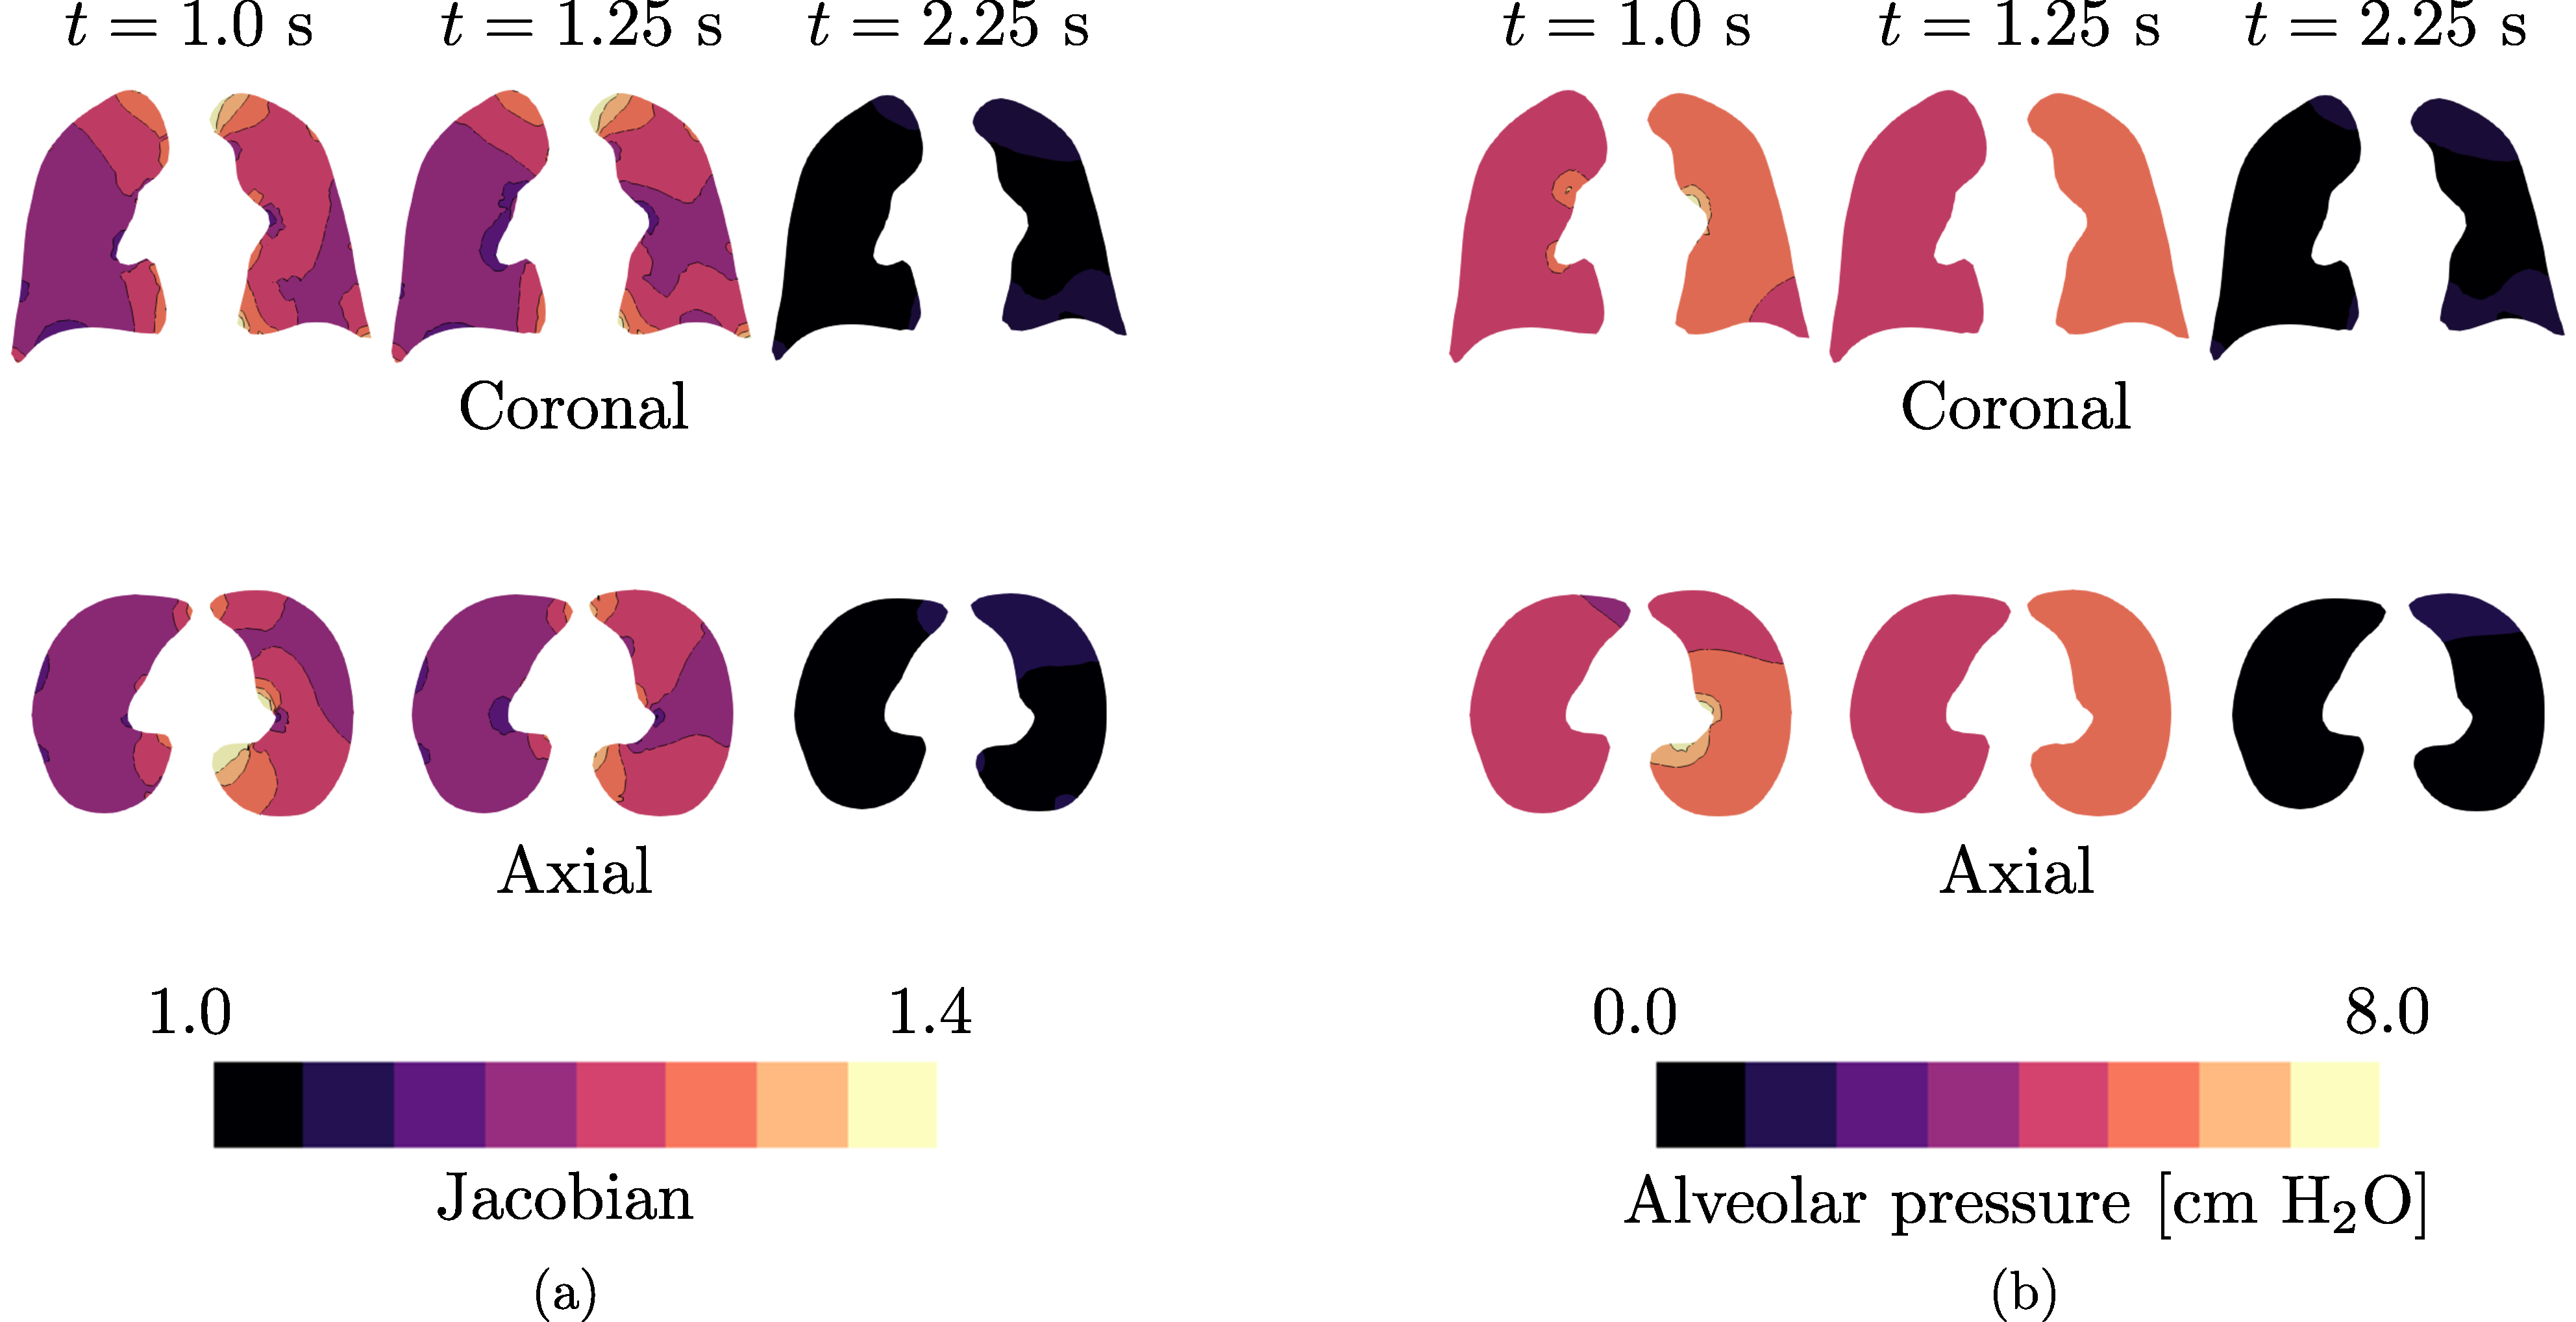
\includegraphics[width=1 \textwidth]{./Figures/jacpres.pdf}
    \caption[]{Temporal evolution during one respiratory cycle of volume-controlled
mechanical ventilation in the baseline case: (a) jacobian field, and (b) alveolar pressure field. Fields are plotted on the current configuration.}
    \label{fig:jac-press-fields}
    \end{center}
\end{figure}

Figure \ref{fig:hyd-por-field} shows the spatiotemporal evolution of the hydrostatic stress and material porosity change fields. High heterogeneity was observed at the end of inspiration and inspiratory pause, with peak hydrostatic-stress values as high as 0.3 kPa, see Figure \ref{fig:hyd-por-field}(a). Material porosity change displayed a spatial distribution and temporal evolution similar to the case of the jacobian field, with positive values everywhere throughout the lung, see Figure \ref{fig:hyd-por-field}(b).


\begin{figure}[h!]
    \begin{center}
    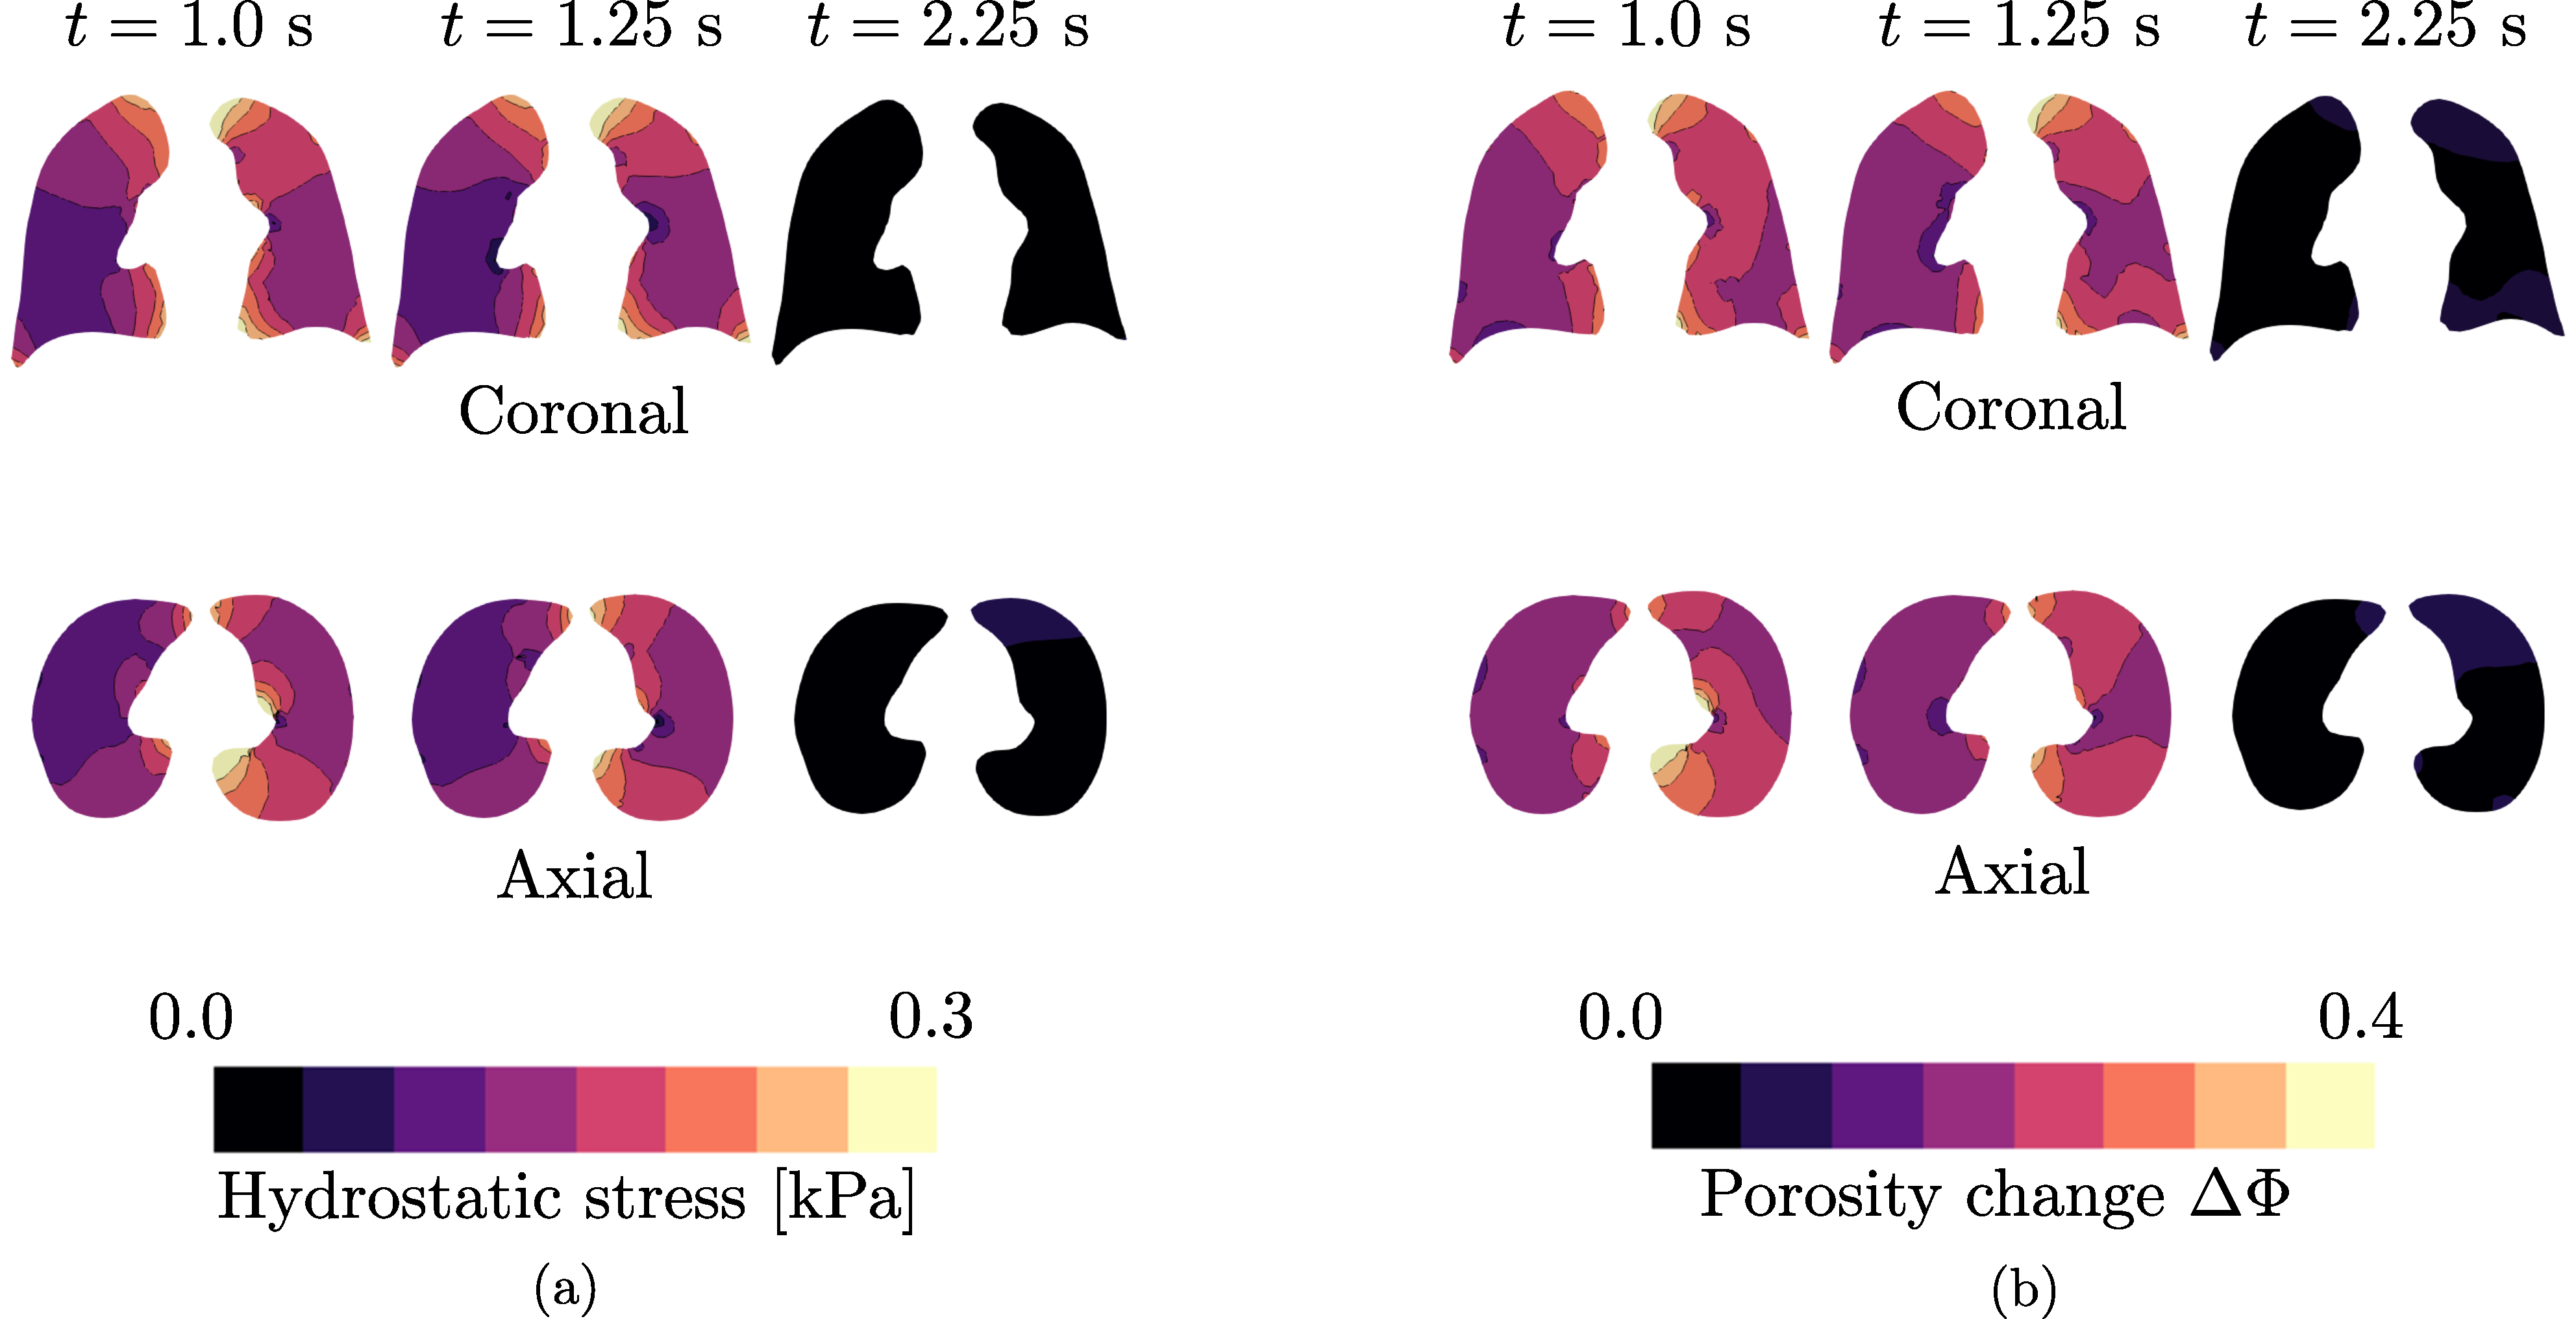
\includegraphics[width=1 \textwidth]{./Figures/hydpor.pdf}
    \caption[]{Temporal evolution during one respiratory cycle of volume-controlled
mechanical ventilation in the  baseline case: (a) hydrostatic stress field, and (b) material porosity change field. Fields are plotted on the current configuration}
    \label{fig:hyd-por-field}
    \end{center}
\end{figure}

%%%%%%%%%%%%%%%%%%%%%%%%%%%%%%%%%%%%%%%%%%%%%%%%%%%%%
%%% Respiratory signals and parameter sensitivity %%%
%%%%%%%%%%%%%%%%%%%%%%%%%%%%%%%%%%%%%%%%%%%%%%%%%%%%%

The airway pressure, flow, and lung volume signals were computed from the lung simulations for all the cases studied. Figure \ref{fig:pcv-resp-mechanics} shows these signals for the case of PCV mode, along with function envelopes that represent the variation of these signals for different levels of variation in the alveolar-wall elasticity and initial alveolar porosity. The flow waveform obtained for the baseline case displays a quick rise and drop following the beginning of the inspiratory (t=0 s) and expiratory (t=1 s) phases, respectively, followed by exponential decay towards zero flow. The time evolution of the volume can also be separated into a saturating exponential curve during the inspiratory phase, followed by an exponential decay towards the resting condition taking place during the expiratory phase. Variations in the alveolar-wall elasticity modulate these responses, as higher values of $\mu$ result in lower flow and lung volume amplitudes, see Figure \ref{fig:pcv-resp-mechanics}(a). In contrast, Figure \ref{fig:pcv-resp-mechanics}(b) shows that an increase in material alveolar porosity causes larger amplitudes in the flow and lung volume signals. 

%%% PCV mode %%%
\begin{figure}[h!]
    \begin{center}
    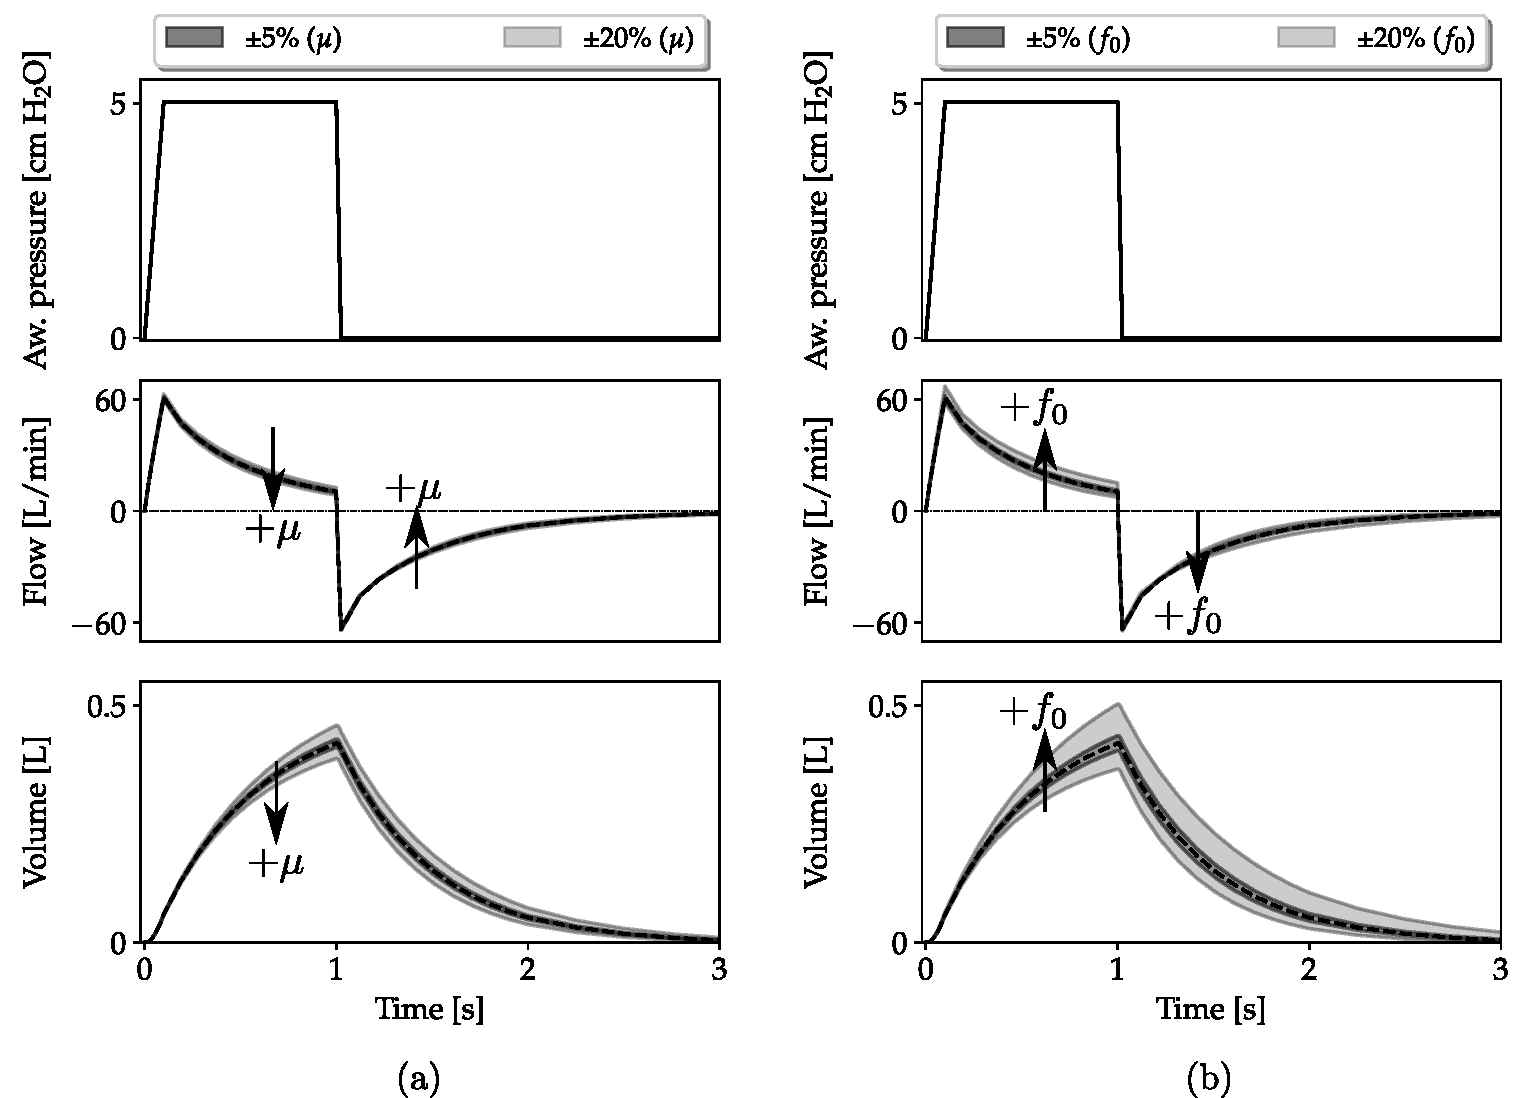
\includegraphics[width=1 \textwidth]{./Figures/SA_pcv.pdf}
    \caption[]{Respiratory signals and parameter sensitivity analysis for pressure-controlled mechanical ventilation: a) variations in the alveolar-wall elasticity, and b) variations in the initial alveolar porosity.  Plots show the time evolution of airway pressure (top), flow (middle), and volume (bottom).}
    \label{fig:pcv-resp-mechanics}
    \end{center}
\end{figure}

Respiratory mechanics curves for the case of the VCV mode are shown in Figure \ref{fig:vcv-resp-mechanics}. During the first phase of constant flow, the volume increases linearly up to the maximum lung volume, while the airway pressure evolves according to a saturating exponential. During the inspiratory (no-flow) pause, pressure rapidly decays to a plateau while lung volume is kept constant. For the expiratory phase, the rapid drop to zero airway pressure causes both the flow and volume to exponentially decay toward their resting values (zero). Figure \ref{fig:vcv-resp-mechanics}(a) shows that increasing the alveolar-wall elasticity results in higher airway-pressure levels during the inspiratory phase, and lower lung volume values during the expiratory phase. In contrast to this trend, an increase in the initial alveolar porosity reduces the amplitude of the airway-pressure signal during inspiration and amplifies the amplitude of the lung-volume signal during expiration, see Figure \ref{fig:vcv-resp-mechanics}(b).      


%%% VCV model %%%
\begin{figure}[h!]
    \begin{center}
    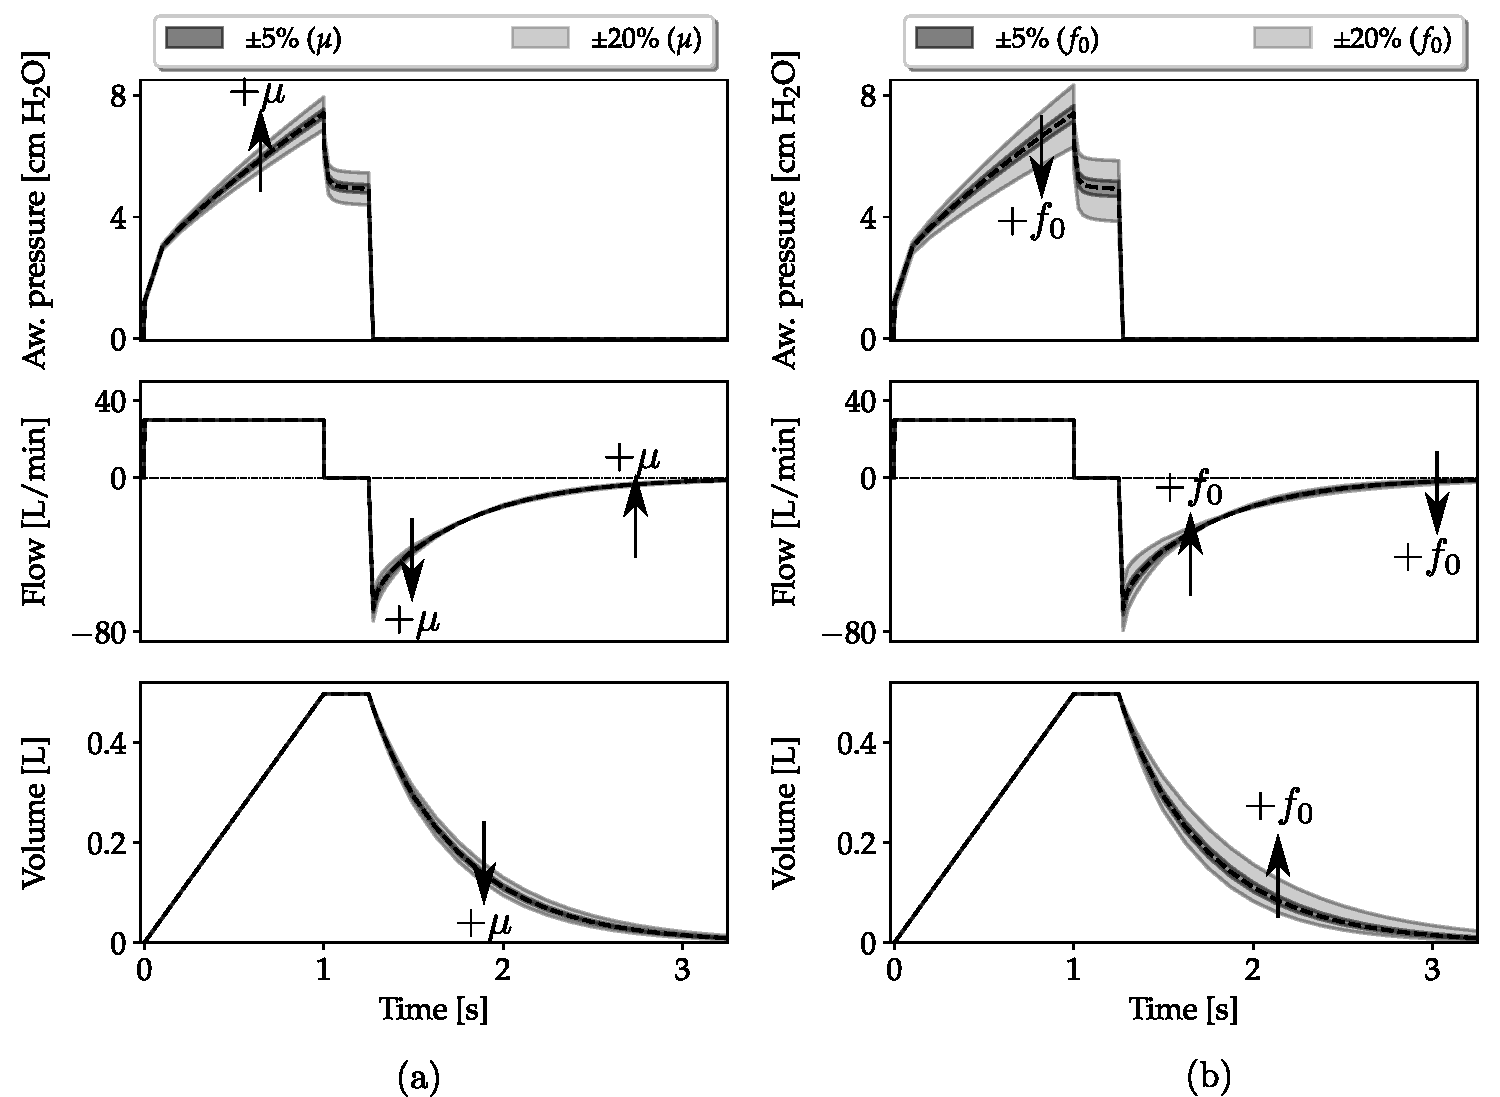
\includegraphics[width=1 \textwidth]{./Figures/SA_vcv.pdf}
    \caption[]{Respiratory signals and parameter sensitivity analysis for volume-controlled mechanical ventilation: a) variations in the alveolar-wall elasticity, and b) variations in the initial alveolar porosity.  Plots show the time evolution of airway pressure (top), flow (middle), and volume (bottom).}
    \label{fig:vcv-resp-mechanics}
    \end{center}
\end{figure}


%%%%%%%%%%%%%%%%%%%%%%%%%%%%%%%%%%%%%%%%%%%%%%%%%%%%%%%%%%%%%%%%%%%%%%%%%%%%%%%%%%
%%% Dependence of respiratory-system compliance on microstructural parameters  %%%
%%%%%%%%%%%%%%%%%%%%%%%%%%%%%%%%%%%%%%%%%%%%%%%%%%%%%%%%%%%%%%%%%%%%%%%%%%%%%%%%%%

To assess the dependence of lung mechanical parameters on microstructural features, we computed the respiratory-system compliance resulting from simulations that considered a range of values of the alveolar-wall elasticity and initial alveolar porosity, see Figure \ref{fig:compliance-relations}(a) and Figure \ref{fig:compliance-relations}(b), respectively. For a fixed baseline value of initial alveolar porosity, the respiratory-system compliance was found to monotonically decrease as alveolar-wall elasticity was increased. When the alveolar-wall elasticity was fixed, the respiratory-system compliance steadily increased as the initial alveolar porosity increased. Both relationships were non-linear in the parameter domain studied.\\     
\begin{figure}[h!]
    \begin{center}
    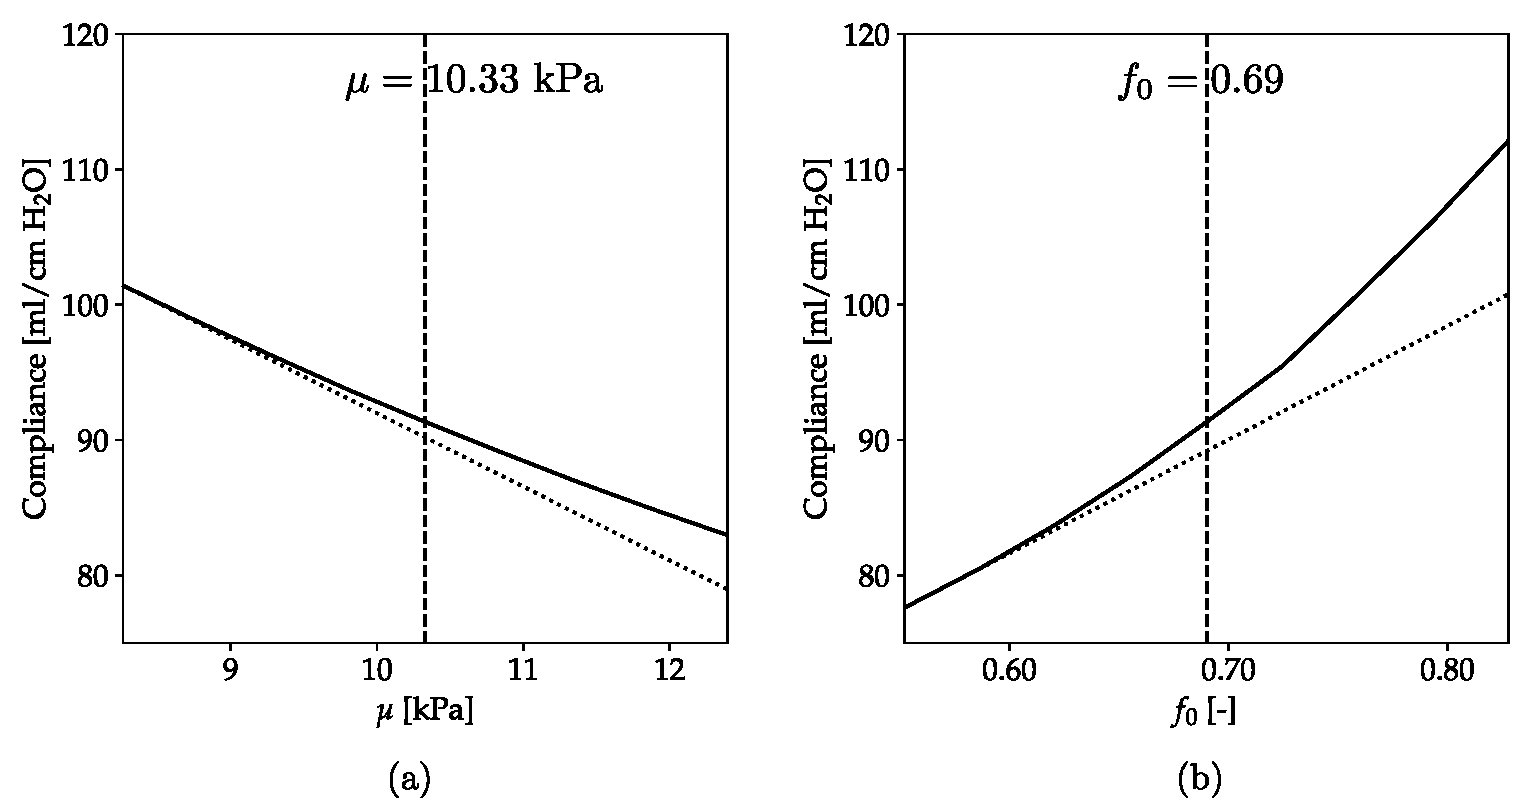
\includegraphics[width=1 \textwidth]{./Figures/SA_compliance.pdf}
    \caption[]{Parameter sensitivity analysis for the respiratory system compliance: a) influence of variations in the alveolar-wall elasticity $\mu$, and b) influence of variations in the initial alveolar porosity $f_0$. Baseline values of both parameters are indicated with a vertical dashed line. Dotted lines are included to visually assess the degree of non-linearity.}
    \label{fig:compliance-relations}
    \end{center}
\end{figure}

%%% quasi-static P-V curve
The influence of alveolar-wall elasticity and alveolar porosity on the quasi-static lung response is shown in Figures \ref{fig:PV-curves}(a) and \ref{fig:PV-curves}(b), respectively. In the case of alveolar-wall elasticity, greater values of $\mu$ resulted in lower lung volumes, for a given airway pressure. When $f_0$ was increased, lung volume increases for a given airway pressure. All pressure-volume curves displayed a non-linear shape.\\

\begin{figure}[h!]
    \begin{center}
    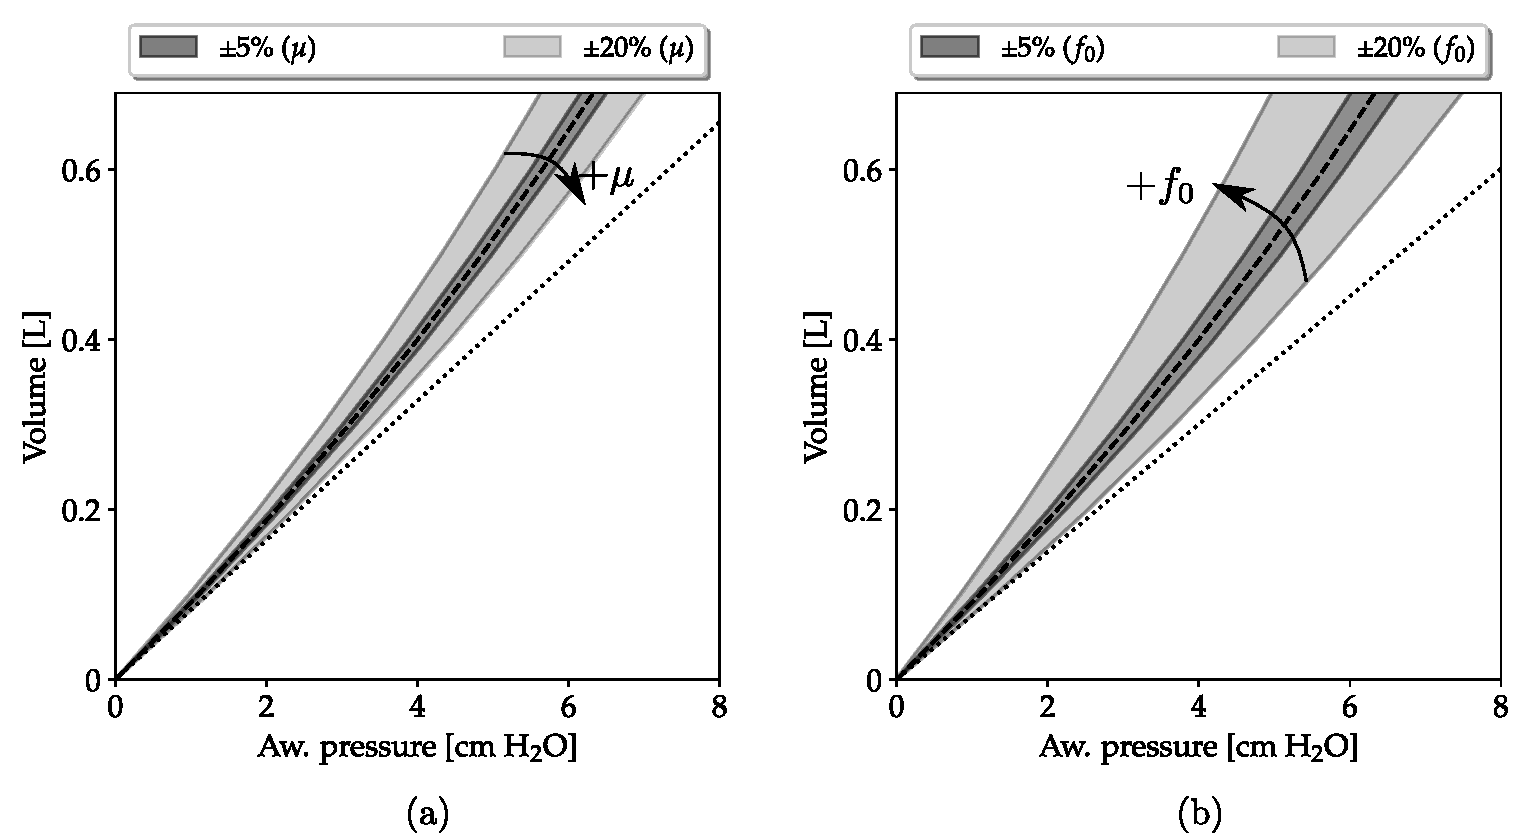
\includegraphics[width=1 \textwidth]{./Figures/SA_super.pdf}
    \caption[]{Quasi-static pressure-volume lung curves and parameter sensitivity analysis: a) variations in the alveolar-wall elasticity, and b) variations in the initial alveolar porosity. Dashed lines represent the baseline case. Dotted lines are included to visually assess the degree of non-linearity.}
    \label{fig:PV-curves}
    \end{center}
\end{figure}

































%\rev{The VCV procedure, another standard mode of mechanical ventilation, in which a target amount of tidal volume (V$_{\text{tidal}}$) is delivered, was also simulated. To resemble this procedure, we consider during the inspiratory phase, a constant prescribed airflow condition as
%\begin{equation}
%\bar{Q}=\frac{\text{V}_\text{tidal}}{\text{A}_\text{aw} \ \text{T}_\text{ins}}, \label{Qpres}
%\end{equation}
%where V$_{\text{tidal}}$ was assumed 500 ml, $\text{T}_\text{insp}$ is the duration of inspiration, assumed 1 second, and $\text{A}_\text {aw}$ is the area of the airway boundary, computed as the surface integral over this boundary. Then, an end-inspiratory pause of 0.25 seconds is performed, in which a null airflow is imposed as $\bar{Q}=0$. Passive expiration was simulated by prescribing $\bar{P}=0$ on the airways boundary for 2 seconds. During inspiration and pause, the ventilation signals are computed as
%\begin{equation}
%\text{P}_\text{aw,sim}(t):=\frac{1}{\text{A}_\text{aw}}\int_{\Gamma_\text{aw}} {P}_{alv} \  d\Gamma_\text{aw}, \label{paw_avg}
%\end{equation}
%\begin{equation}
%    \text{V}_{\text{sim}}(t):= \int_{[0,t]} \bar{Q}\ d\tau ,
%\end{equation} 
%\begin{equation}
%    \dot{\rm{V}}_{\rm sim}(t):= \bar{Q}.
%\end{equation}
%while for the expiratory phase, the simulated signals are given by equations \ref{pawsim}-\ref{eq:Qsum}. Figure \ref{fig:VCV} shows the sensitive analysis of ventilator signals during the entire respiratory cycle. In this case, to introduce 500 ml of air, a lower pressure is necessary for more porous microstructures, which expel the air more slowly, trapping small volumes. Concerning alveolar-wall elasticity, lungs with higher $\mu$ values reach a higher peak pressure and are faster in the expiratory phase. }

%\rev{The PCV protocol corresponds to a standard mode of mechanical ventilation, in which the ventilator controls airway pressure while airflow and volume are dependent variables \cite{ashworth2018clinical}. The details of the necessary considerations for its modeling under a poromechanical framework were discussed in  \citet{avileshurtado2022whole}, so these are only briefly presented here. 

%To simulate the PCV mode, we prescribe a time-varying pressure condition at the airway boundary, miming the ventilator's effect. At the beginning of inspiration, the pressure rises linearly until it reaches a peak value of 5 cm H$_2$0 in 0.1 seconds, a pressure that is maintained until the end of inspiration, whose duration was set at 1 second. Then, this pressure is suddenly reduced to zero and is maintained at this value for the next 2 seconds, corresponding to the expiratory phase. After solving the finite element problem, the signals airway pressure ($\text{P}_{\text{aw,sim}}$), flow ($\dot{\text{V}}_{ \text{sim}}$) and volume (${\text{V}}_{\text{sim}}$) were obtained as}

%\begin{equation}
%\text{P}_\text{aw,sim}(t):=\bar{P}, \label{pawsim}
%\end{equation}

%\begin{equation}
%    \text{V}_{\text{sim}}(t):= \int_{\Omega_0} J \, d\Omega_0 - \int_{\Omega_0}  \, d\Omega_0, \label{Vsim}
%\end{equation}
%and
%\begin{equation}
%    \dot{\rm{V}}_{\rm sim}(t):= \int_{\Gamma_\text{aw}} \vec Q \cdot \vec N \, d \Gamma_\text{aw} = \pd{\rm{V}_{\rm sim}}{t},
%    \label{eq:Qsum}
%\end{equation}
%\rev{where in the last equality, the incompressibility of both phases has been considered, and $\Gamma_\text{aw}$ is the airway boundary. Figure \ref{fig:PCV} shows the signals resulting from the sensitivity analysis of both parameters. In this Figure, the relative variations corresponding to $\pm$20\% are plotted in a light color. In addition, variations of $\pm$5\% are indicated, plotted in dark color. It is observed that an increase in $\mu$ induces smaller volumes and slight reductions in the magnitude of the flow throughout the respiratory cycle. The opposite is observed about $f_0$, apparently having a more significant influence during PCV in the range of values considered.}\\

















%Option 2
%\begin{figure}[h!]
%    \begin{center}
%    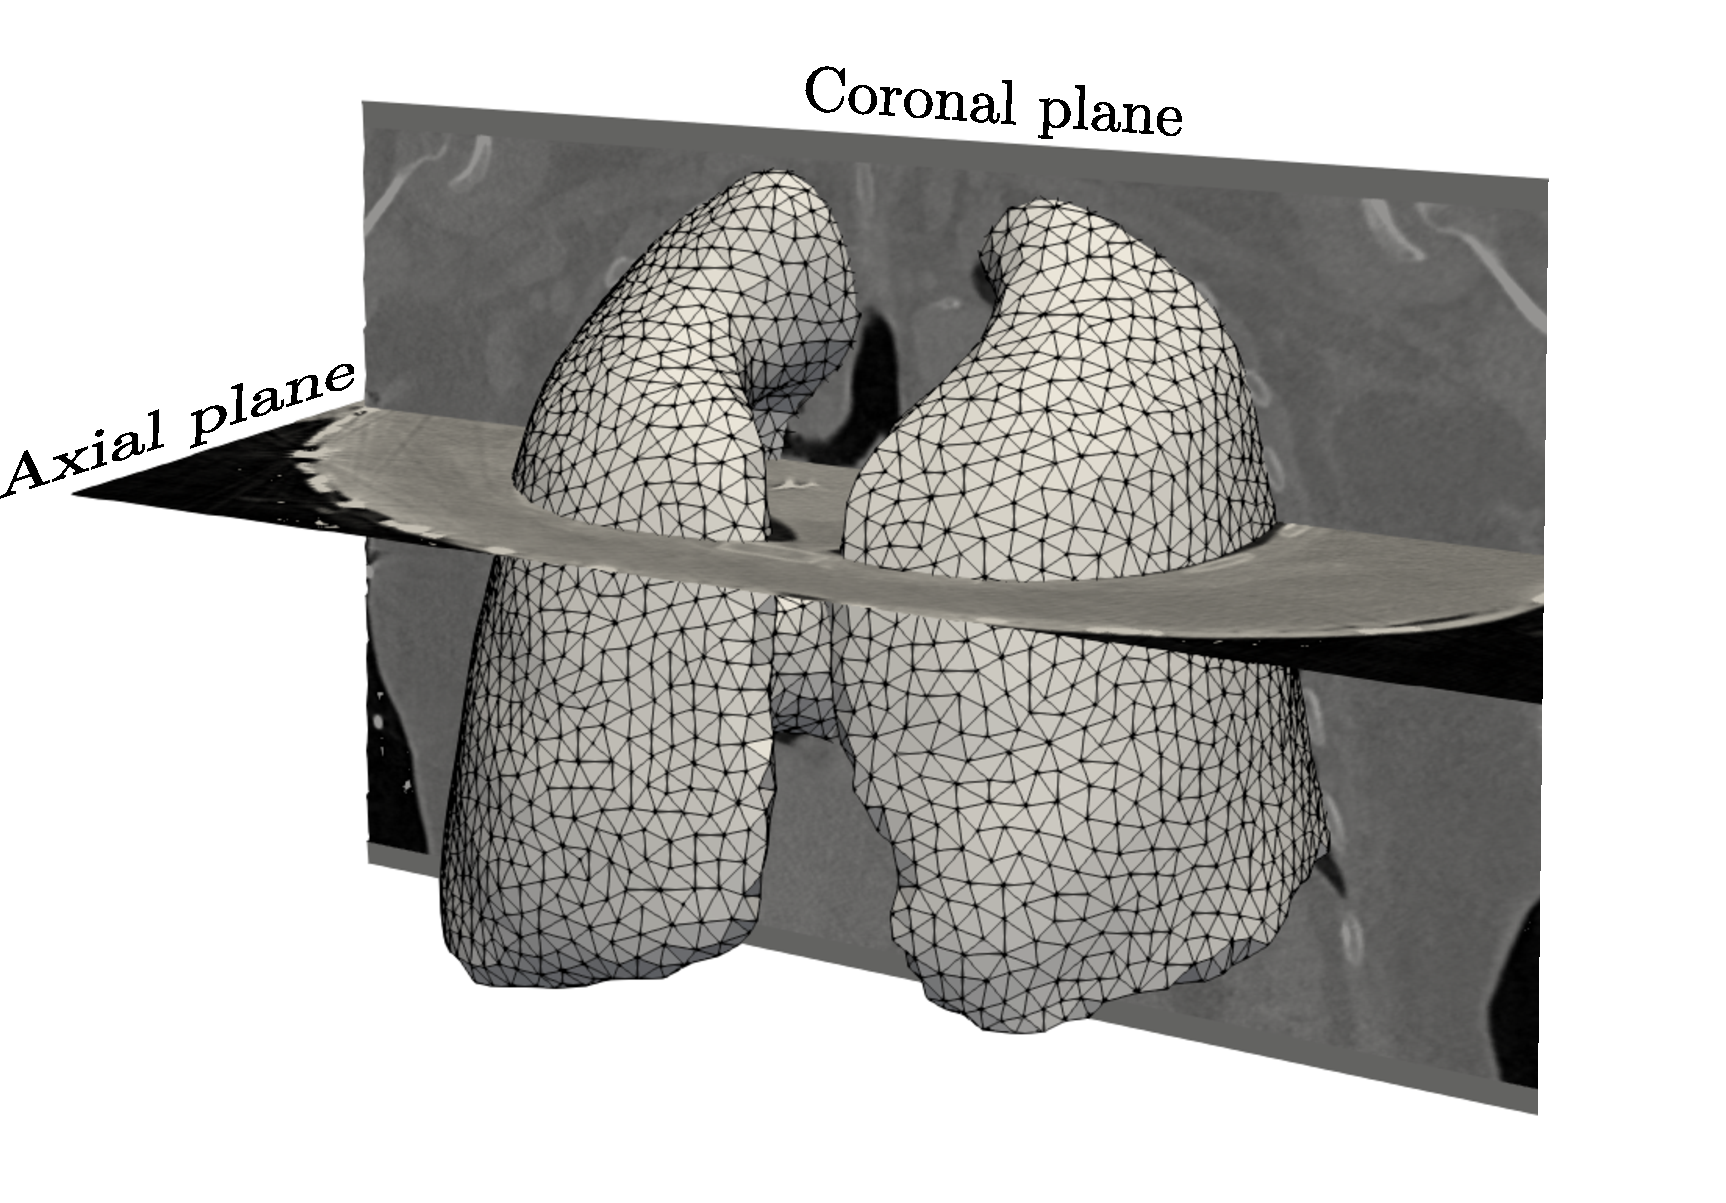
\includegraphics[width=0.45 %\textwidth]{./Figures/mesh2.pdf}
%    \caption[]{\rev{Whole-lung finite element %mesh with coronal and axial planes used for %analysis}}
%    \label{fig:mesh}
%    \end{center}
%\end{figure}



%For the TKD model that represents the alveolar response, we considered the following parameter values $\mu=10.33$ kPa, $f_0=0.69$, $\alpha=10.05$ and $d=0.56$. The alveolar-wall elasticity

%\rev{In order to test the fidelity of our multiscale framework, we constructed whole-lung models from computed tomography images of real patients at the end of the expiratory phase, a condition that was assumed as the reference configuration of the lung. Using the ITK segmentation tools, we identified the lung domain, and then with the CGAL Library, a tetrahedral mesh was constructed from the segmented images. Following our previous contribution \cite{avileshurtado2022whole}, the boundary of the lung domain was partitioned into the airways surface and the visceral pleura. To mimic the interaction between the ventilator and lung patient, the air was only allowed to enter or exit through the airways boundary, where pressure or flow was prescribed, depending on the considered application. In addition, the mechanical effect of the rib cage and the mediastinum on the lung was considered by employing a Robin boundary condition of the form
%	 \begin{equation}
%	     \bar{\vec{T}}^c(\vec X)={K}_\text{s} \left\{\vec{\varphi(\vec X) -X} \right\},
%	 \end{equation}
%which is prescribed on the entire surface. In our simulations we have used ${K}_\text{s}=80\cdot 10^{–3}$ kPa/mm, which allows us to represent the chest-wall compliance in normal subjects \cite{avileshurtado2022whole}. }
 
%   \begin{figure}[h!]
% 	\begin{center}
% 		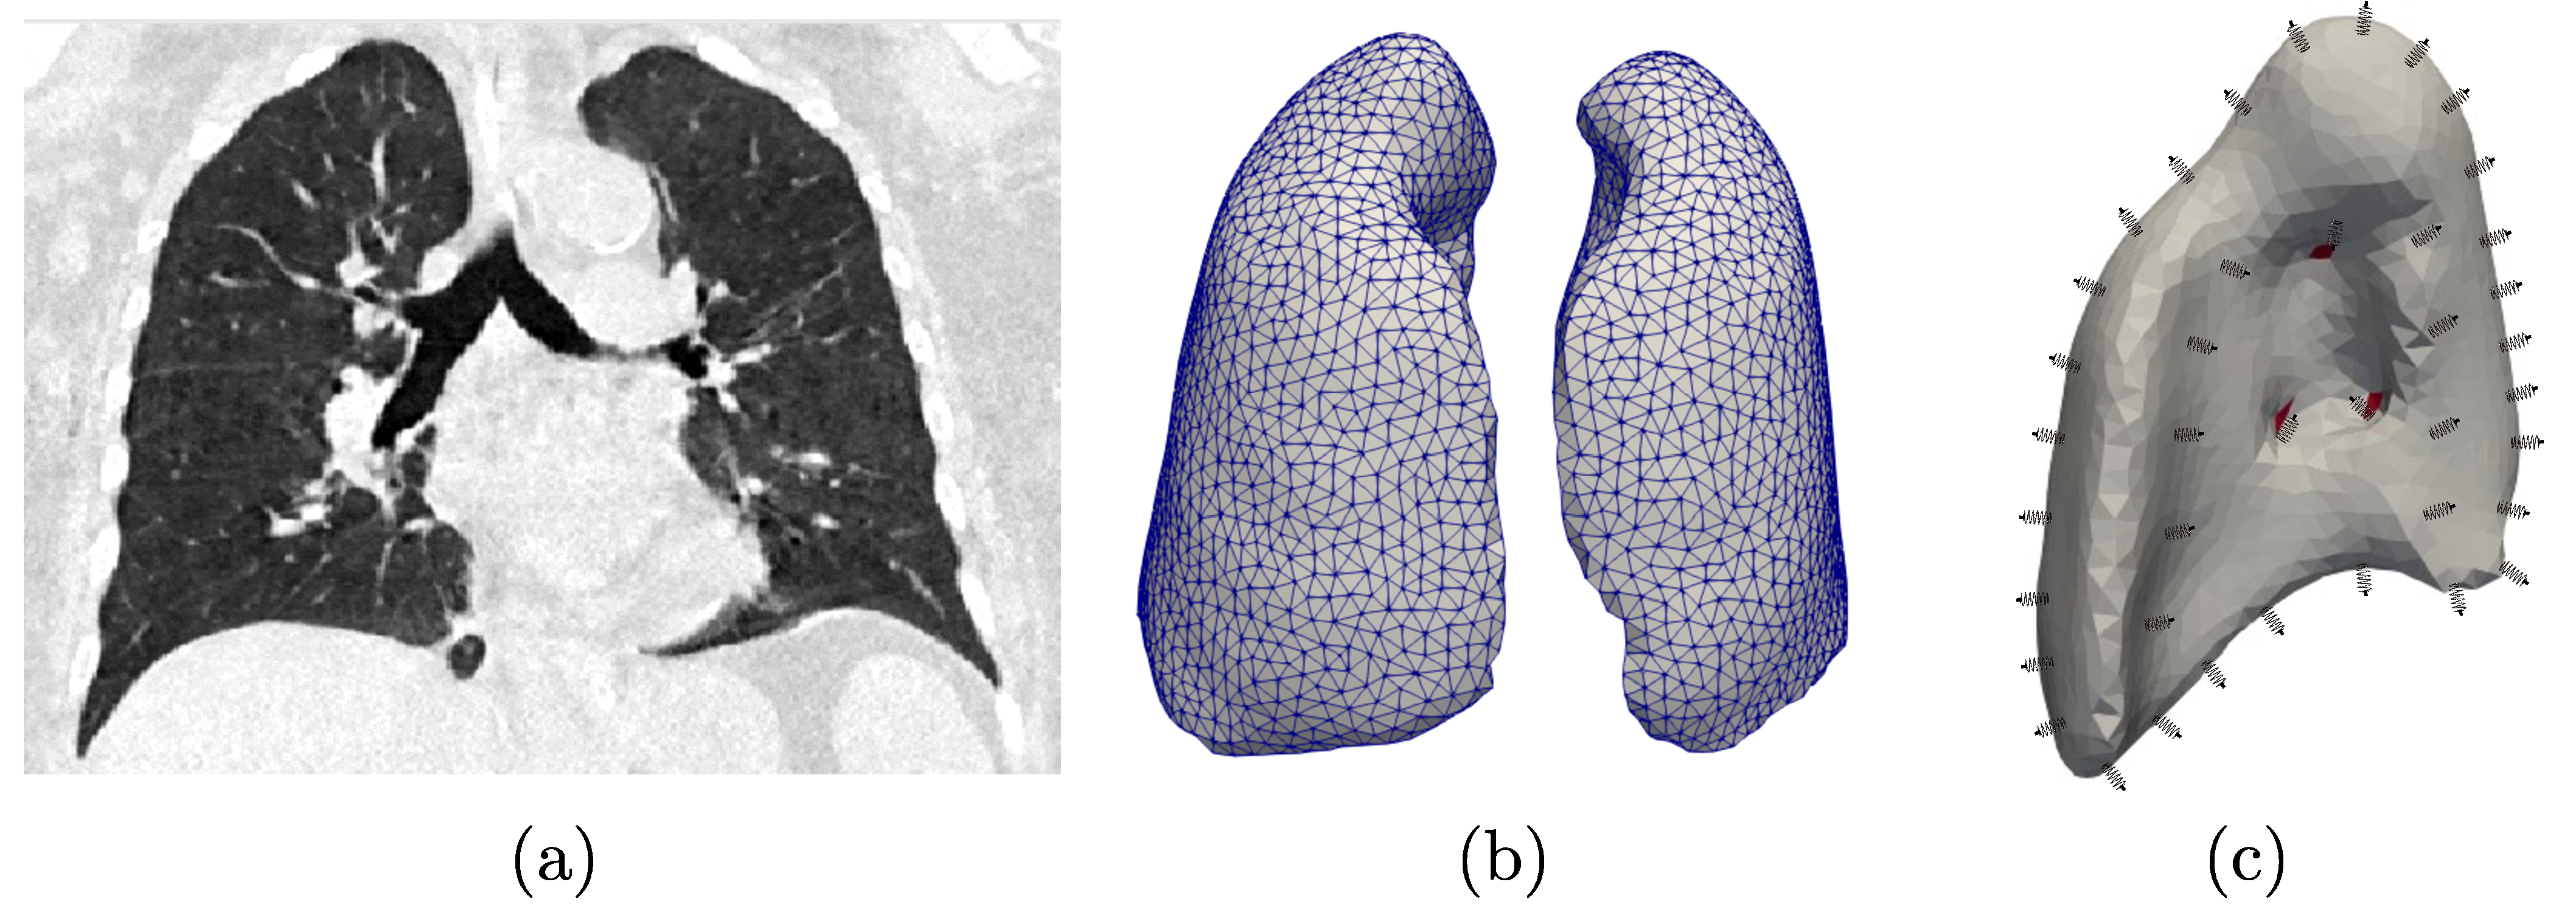
\includegraphics[width=0.8 \textwidth]{./Figures/fig02_geom.pdf}
% 	\caption[]{(a) CT image of the lung. (b) Mesh for macroscopic lung  model. (c) Boundaries considered for right lung. The airways boundary is shown in red. PREGUNTAR QUE FIGURA PONER}
% 	\label{fig:geom}
% 	\end{center}
% \end{figure}

%\rev{The TKD unit cell allows to represent the alveolar microstructure suitably and depends on four parameters called alveolar-wall elasticity ($\mu$), initial tissue porosity ($f_0$), rotational stiffness coefficient ($\alpha$), and the overlap coefficient ($d$). Following \citet{concha2020upscaling}, we consider $\mu=10.33$ kPa, $f_0=0.69$, $\alpha=10.05$ and $d=0.56$. In addition, the TKD model allows incorporating prestress set at 0.5  kPa for our simulations. We remark that in the TKD, the parameters $f_0$ and $\mu$ have a leading role in the micromechanical response, as previously shown for different load conditions \cite{ConchaEtAl2018,concha2020upscaling}. In order to study the influence of these two parameters on the whole-lung response, we performed sensitivity analyses on relevant clinical experiments called pressure control mechanical ventilation (PCV), volume control mechanical ventilation (VCV), and construction of pressure-volume curves using the supersyringe method. For this, we consider variations $\pm$ 20\%, corresponding to ranges of $[0.55,0.83]$ and $[8.3,12.4]$ kPa for $f_0$ and $\mu$ respectively.}\\

%\rev{The PCV protocol corresponds to a standard mode of mechanical ventilation, in which the ventilator controls airway pressure while airflow and volume are dependent variables \cite{ashworth2018clinical}. The details of the necessary considerations for its modeling under a poromechanical framework were discussed in  \citet{avileshurtado2022whole}, so these are only briefly presented here. To simulate the PCV mode, we prescribe a time-varying pressure condition at the airway boundary, miming the ventilator's effect. At the beginning of inspiration, the pressure rises linearly until it reaches a peak value of 5 cm H$_2$0 in 0.1 seconds, a pressure that is maintained until the end of inspiration, whose duration was set at 1 second. Then, this pressure is suddenly reduced to zero and is maintained at this value for the next 2 seconds, corresponding to the expiratory phase. After solving the finite element problem, the signals airway pressure ($\text{P}_{\text{aw,sim}}$), flow ($\dot{\text{V}}_{ \text{sim}}$) and volume (${\text{V}}_{\text{sim}}$) were obtained as}

%\begin{equation}
%\text{P}_\text{aw,sim}(t):=\bar{P}, \label{pawsim}
%\end{equation}

%\begin{equation}
%    \text{V}_{\text{sim}}(t):= \int_{\Omega_0} J \, d\Omega_0 - %\int_{\Omega_0}  \, d\Omega_0, \label{Vsim}
%\end{equation}
%and
%\begin{equation}
%    \dot{\rm{V}}_{\rm sim}(t):= \int_{\Gamma_\text{aw}} \vec Q \cdot \vec N %\, d \Gamma_\text{aw} = \pd{\rm{V}_{\rm sim}}{t},
%    \label{eq:Qsum}
%\end{equation}
%\rev{where in the last equality, the incompressibility of both phases has been considered, and $\Gamma_\text{aw}$ is the airway boundary. Figure \ref{fig:PCV} shows the signals resulting from the sensitivity analysis of both parameters. In this Figure, the relative variations corresponding to $\pm$20\% are plotted in a light color. In addition, variations of $\pm$5\% are indicated, plotted in dark color. It is observed that an increase in $\mu$ induces smaller volumes and slight reductions in the magnitude of the flow throughout the respiratory cycle. The opposite is observed about $f_0$, apparently having a more significant influence during PCV in the range of values considered.}\\
%\begin{figure}[h!]
%    \begin{center}
%    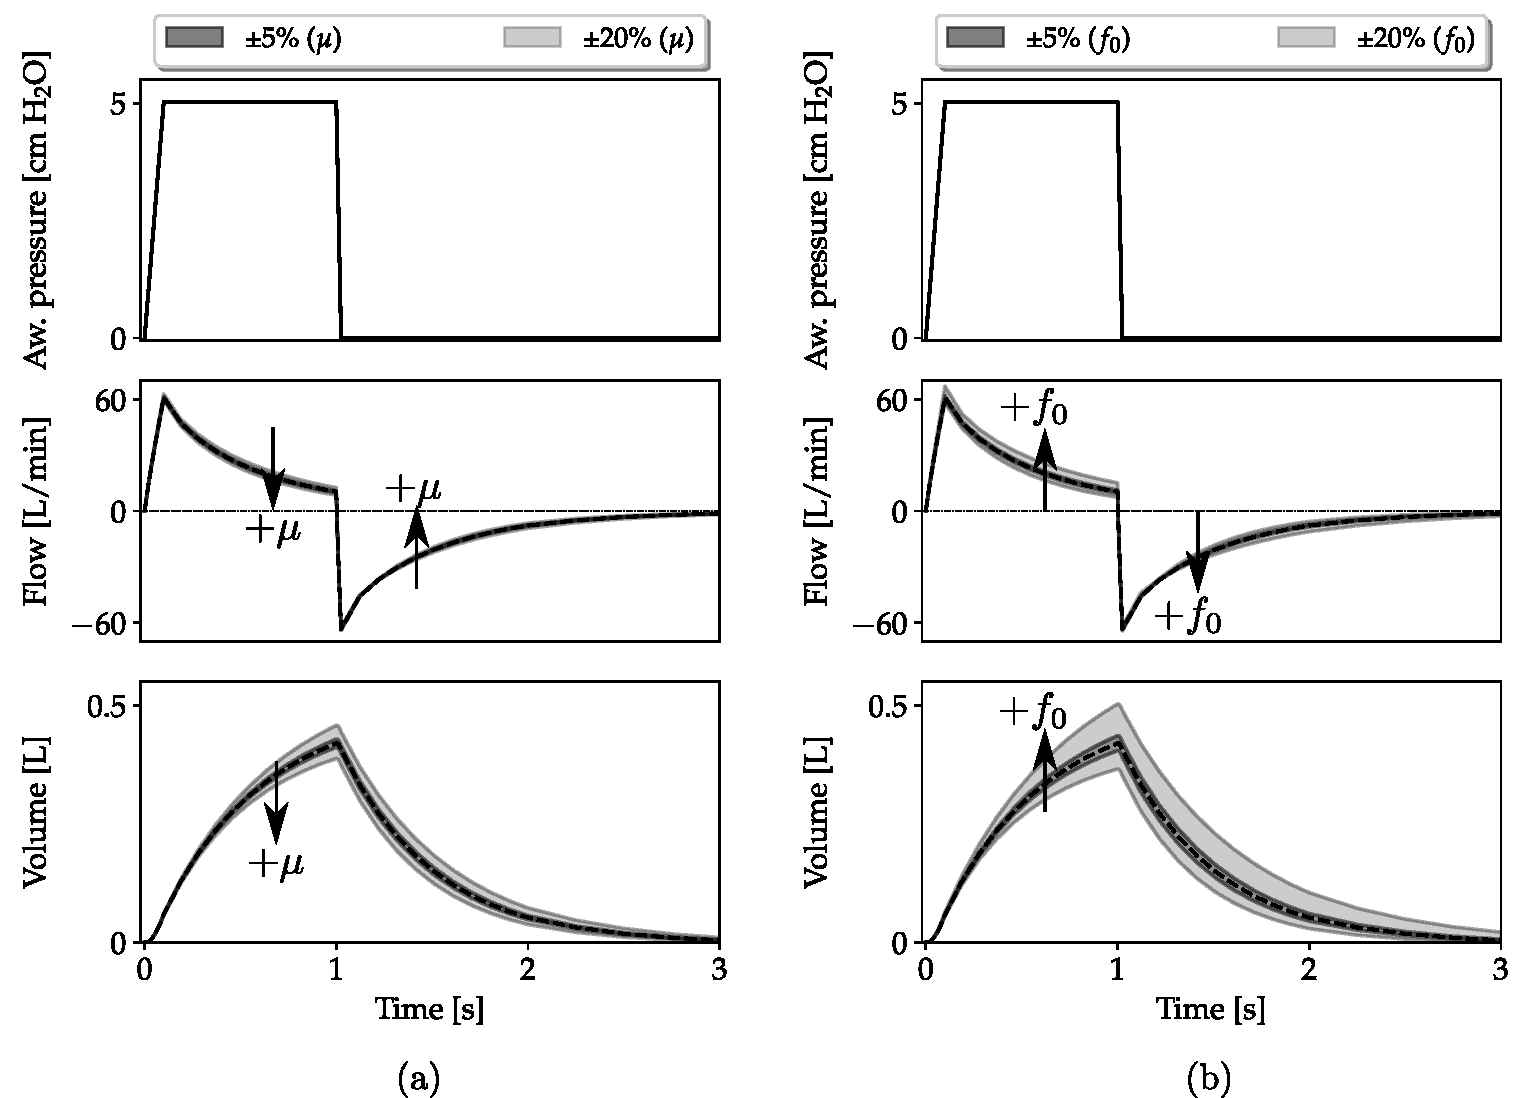
\includegraphics[width=1 \textwidth]{./Figures/SA_pcv.pdf}
%    \caption[]{\rev{Parameter sensitivity analysis for pressure-controlled mechanical ventilation: a) variations in the alveolar-wall elasticity, and b) variations in the initial tissue porosity.  Plots show the time evolution of airway pressure (top), flow (middle), and volume (bottom).}}
%    \label{fig:PCV}
%    \end{center}
%\end{figure}








%\rev{
%The importance of microstructure in relevant clinical macroscopic parameters, such as respiratory system compliance (C$_\text{rs}$), was also studied. To this end, we perform a least squares fit to each set of signals $\text{P}_{\text{aw,sim}}$, $\dot{\text{V}}_{\text{sim }}$, ${\text{V}}_{\text{sim}}$, where following \citep{Bates2009} we want to minimize the objective function \begin{equation} S=\sum_{t_i=0}^\text{T}\left[ \text{P}_\text{aw,sim} (t_i) - \frac{\text{V}_\text {sim}( t_i)}{\text{C}_{\text{rs}}}+ \text{R} \dot{\text{V}}_{\text{sim}}(t_i) \right]^2, \end{equation} with R the airway resistance, which is also determined by the least squares fit. As discussed in \citet{avileshurtado2022whole}, for a poroelastic model, this parameter is mainly affected by the permeability tensor, which has been assumed constant in this work. Therefore, it is expected that the variations of R are not significant. The influence of the variation of $\mu$ and $f_0$ on the value of C$_\text{rs}$ is shown in Figure \ref{fig:compliance}. Consistent with PCV signals, an increase in $f_0$ is related to more compliant (less stiff) lungs, while an increase in $\mu$ reduces its value. } \\
%\begin{figure}[h!]
%    \begin{center}
%    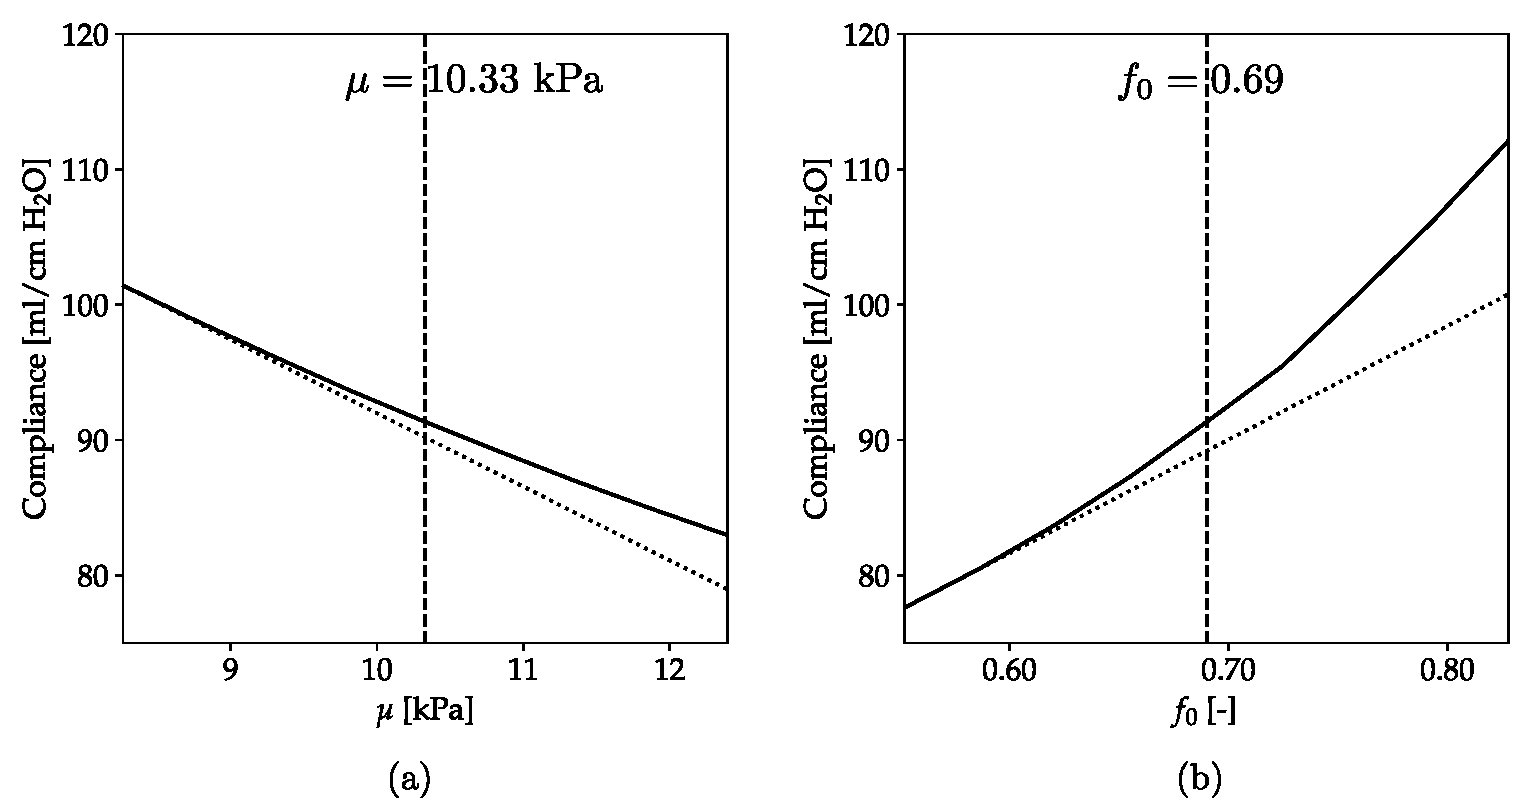
\includegraphics[width=1 \textwidth]{./Figures/SA_compliance.pdf}
%    \caption[]{\rev{Parameter sensitivity analysis for the respiratory system compliance: a) variations in the alveolar-wall elasticity, and b) variations in the initial tissue porosity. Base values of both parameters are indicated with a dotted line.}}
%    \label{fig:compliance}
%    \end{center}
%\end{figure}


%\rev{The VCV procedure, another standard mode of mechanical ventilation, in which a target amount of tidal volume (V$_{\text{tidal}}$) is delivered, was also simulated. To resemble this procedure, we consider during the inspiratory phase, a constant prescribed airflow condition as
%\begin{equation}
%\bar{Q}=\frac{\text{V}_\text{tidal}}{\text{A}_\text{aw} \ %\text{T}_\text{ins}}, \label{Qpres}
%\end{equation}
%where V$_{\text{tidal}}$ was assumed 500 ml, $\text{T}_\text{insp}$ is the duration of inspiration, assumed 1 second, and $\text{A}_\text {aw}$ is the area of the airway boundary, computed as the surface integral over this boundary. Then, an end-inspiratory pause of 0.25 seconds is performed, in which a null airflow is imposed as $\bar{Q}=0$. Passive expiration was simulated by prescribing $\bar{P}=0$ on the airways boundary for 2 seconds. During inspiration and pause, the ventilation signals are computed as
%\begin{equation}
%\text{P}_\text{aw,sim}(t):=\frac{1}{\text{A}_\text{aw}}\int_{\Gamma_\text{aw}} {P}_{alv} \  d\Gamma_\text{aw}, \label{paw_avg}
%\end{equation}
%\begin{equation}
 %   \text{V}_{\text{sim}}(t):= \int_{[0,t]} \bar{Q}\ d\tau ,
%\end{equation} 
%\begin{equation}
%    \dot{\rm{V}}_{\rm sim}(t):= \bar{Q}.
%\end{equation}
%while for the expiratory phase, the simulated signals are given by equations \ref{pawsim}-\ref{eq:Qsum}. Figure \ref{fig:VCV} shows the sensitive analysis of ventilator signals during the entire respiratory cycle. In this case, to introduce 500 ml of air, a lower pressure is necessary for more porous microstructures, which expel the air more slowly, trapping small volumes. Concerning alveolar-wall elasticity, lungs with higher $\mu$ values reach a higher peak pressure and are faster in the expiratory phase. }  \\
%\begin{figure}[h!]
%    \begin{center}
%    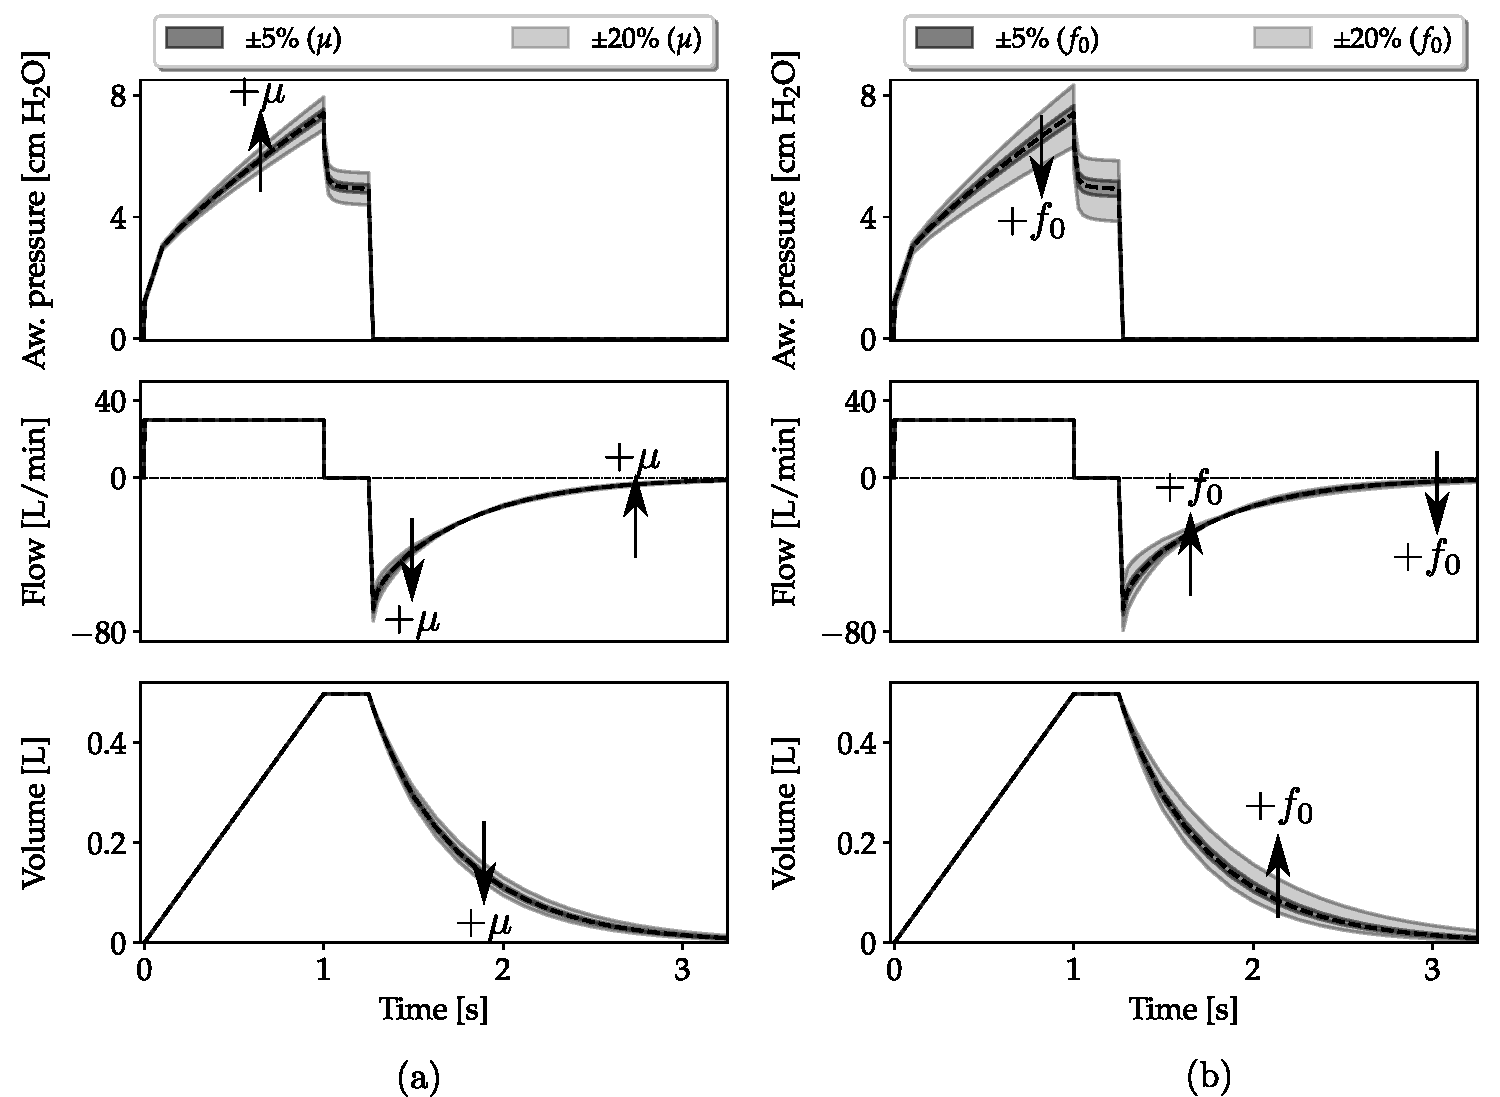
\includegraphics[width=1 \textwidth]{./Figures/SA_vcv.pdf}
%    \caption[]{\rev{Parameter sensitivity analysis for volume-controlled mechanical ventilation: a) variations in the alveolar-wall elasticity, and b) variations in the initial tissue porosity.  Plots show the time evolution of airway pressure (top), flow (middle), and volume (bottom).}}
%    \label{fig:VCV}
%    \end{center}
%\end{figure}

%\rev{Our model can also predict the temporal evolution of 3D relevant physical quantities during mechanical ventilation. Figure \ref{fig:fields} shows the spatial distribution of the alveolar pressure and Material porosity change defined as $\Delta \Phi=\Phi-\Phi_0$ for the base case $\mu=10.33$ kPa and $f_0=0.69$. Note that $\Phi_0=f_0$. Three instants during the VCV simulation are considered: the end of inspiration ($t_1:=1.0$ s), the end of the end-inspiratory pause ($t_2:=1.25$ s), and when half expiration has elapsed ($t_3:= 2.25$ s). The maximum values of the Material porosity change and pressure fields are reached at $t_1$ and are slightly reduced at $t_2$. Note that at $t_2$, the alveolar pressure is uniform in each lung; in contrast, the Material porosity change is heterogeneous. During $t_3$, the porosity change and pressures are strongly reduced, presenting values less than 0.2 and 2 cm H$_2$O, respectively.} \\

%\begin{figure}[h!]
%    \begin{center}
%    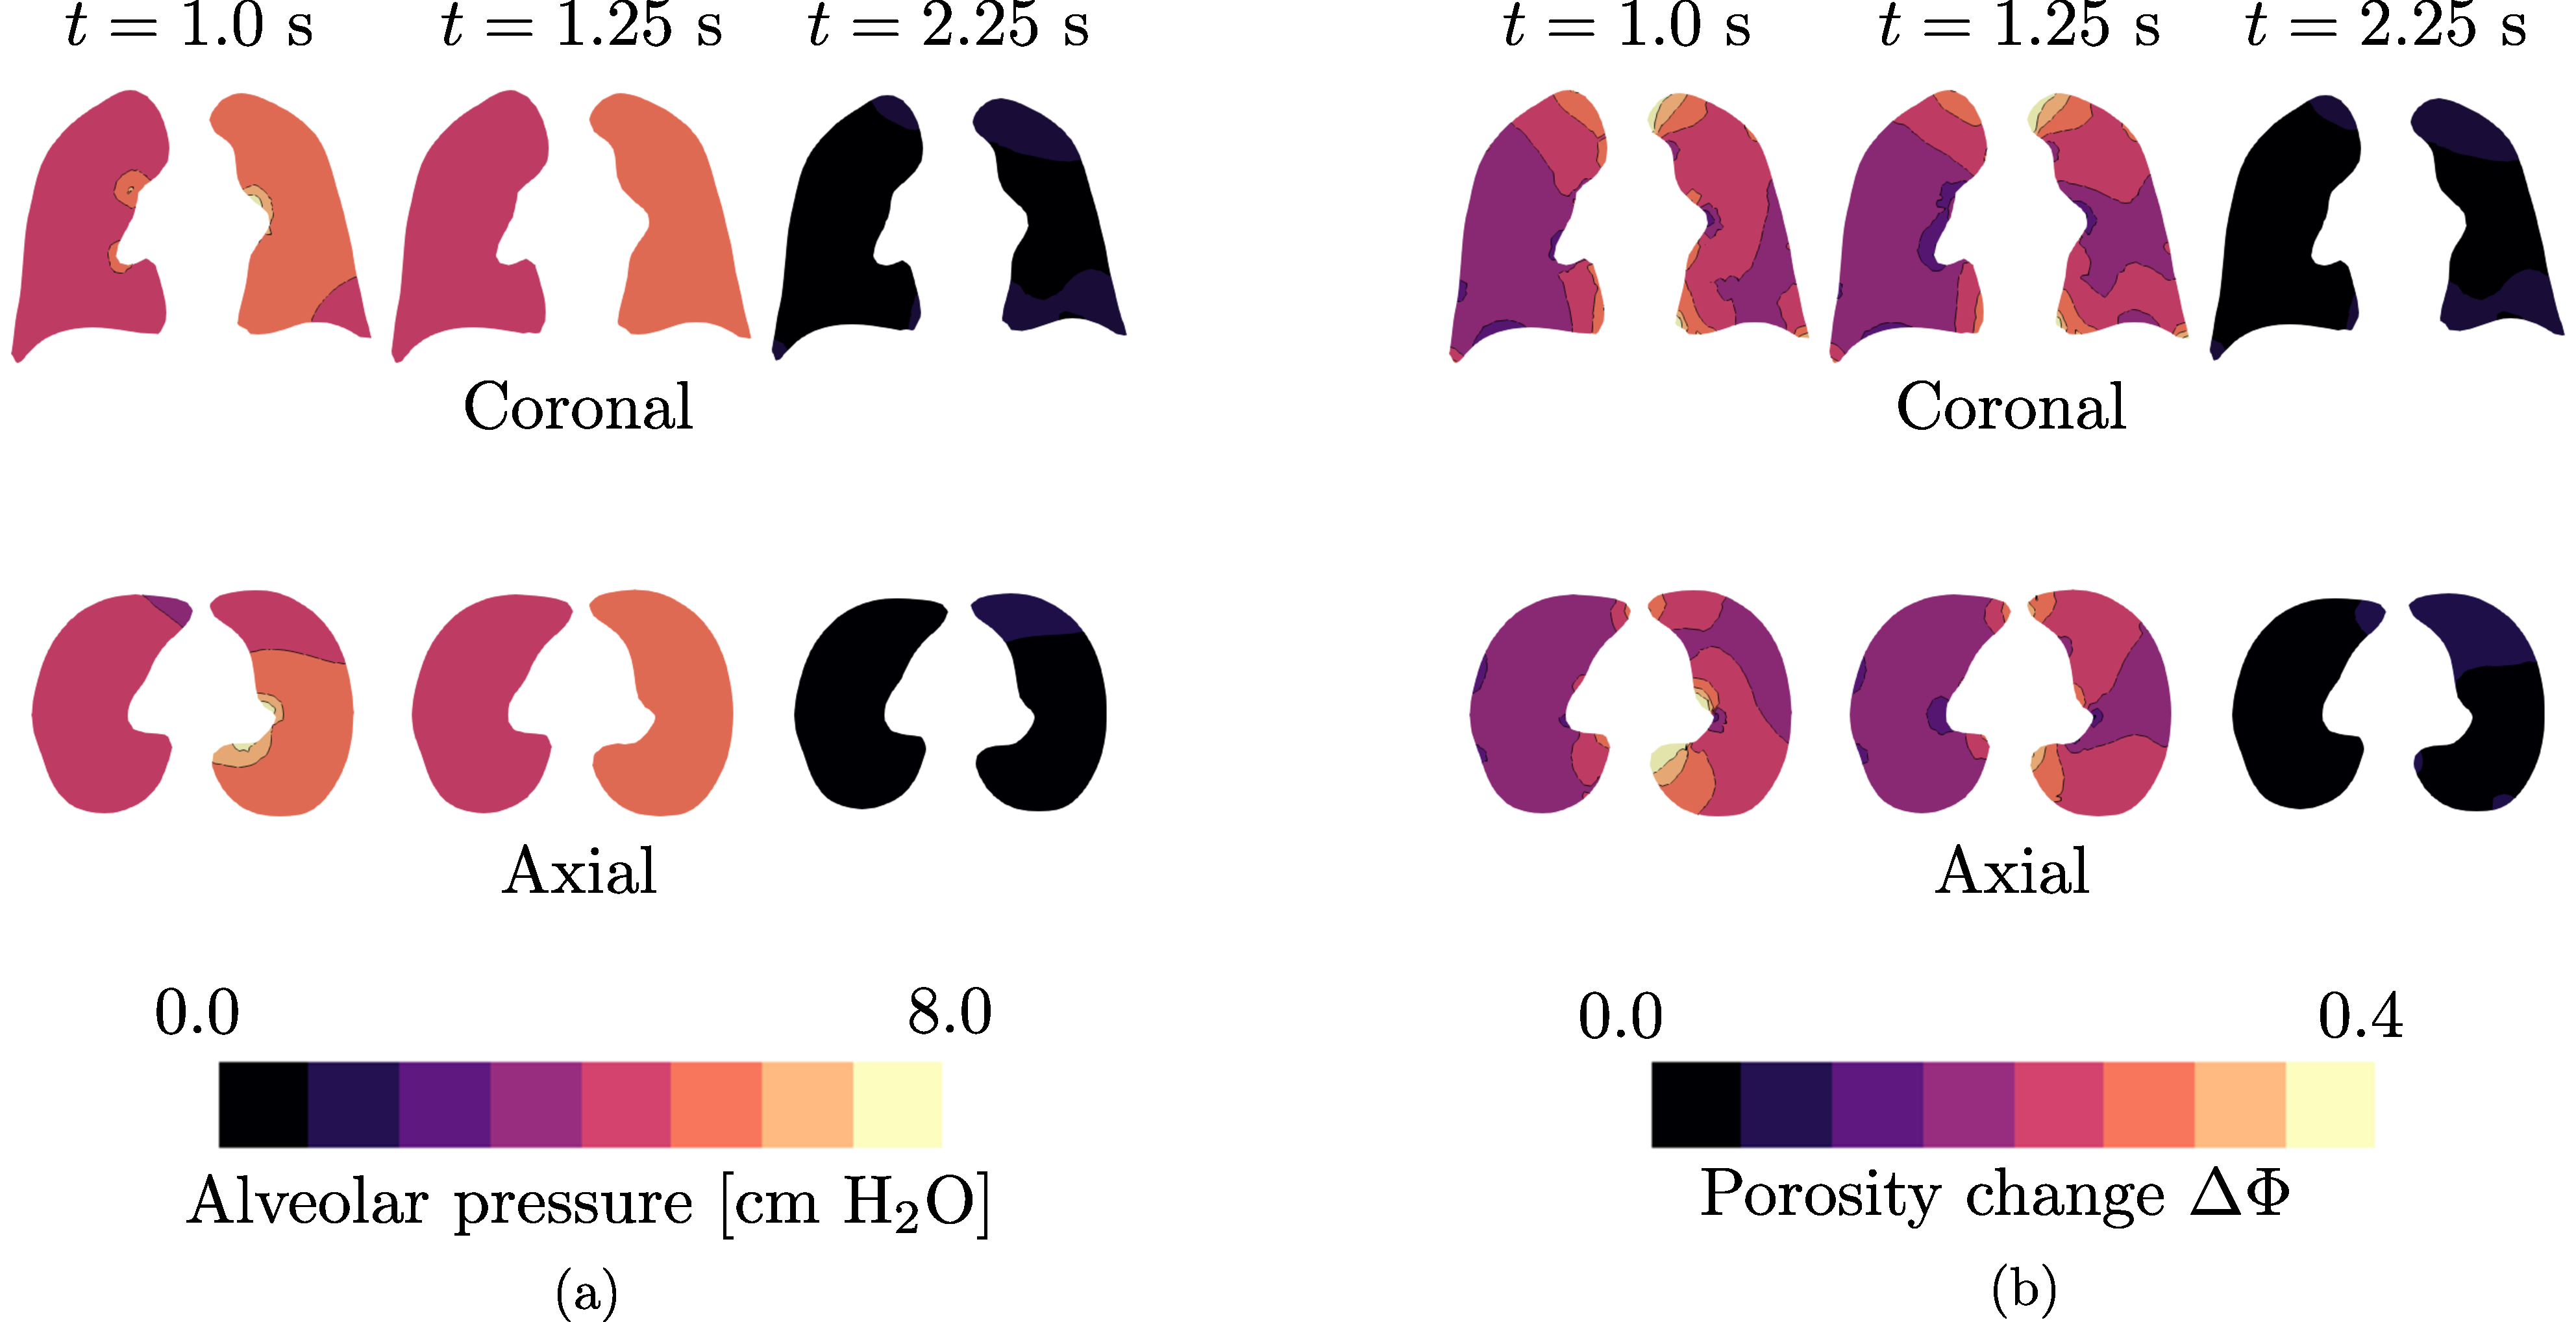
\includegraphics[width=1 \textwidth]{./Figures/prespor.pdf}
%    \caption[]{\rev{Temporal evolution during one respiratory cycle of volume-controlled
%mechanical ventilation for the case $\mu=10.33$ kPa and $f_0=0.69$: (a) alveolar pressure, and (b)  Material porosity change. Fields are plotted in the current configuration}}
%    \label{fig:fields}
%    \end{center}
%\end{figure}

%\begin{figure}[h!]
%    \begin{center}
%    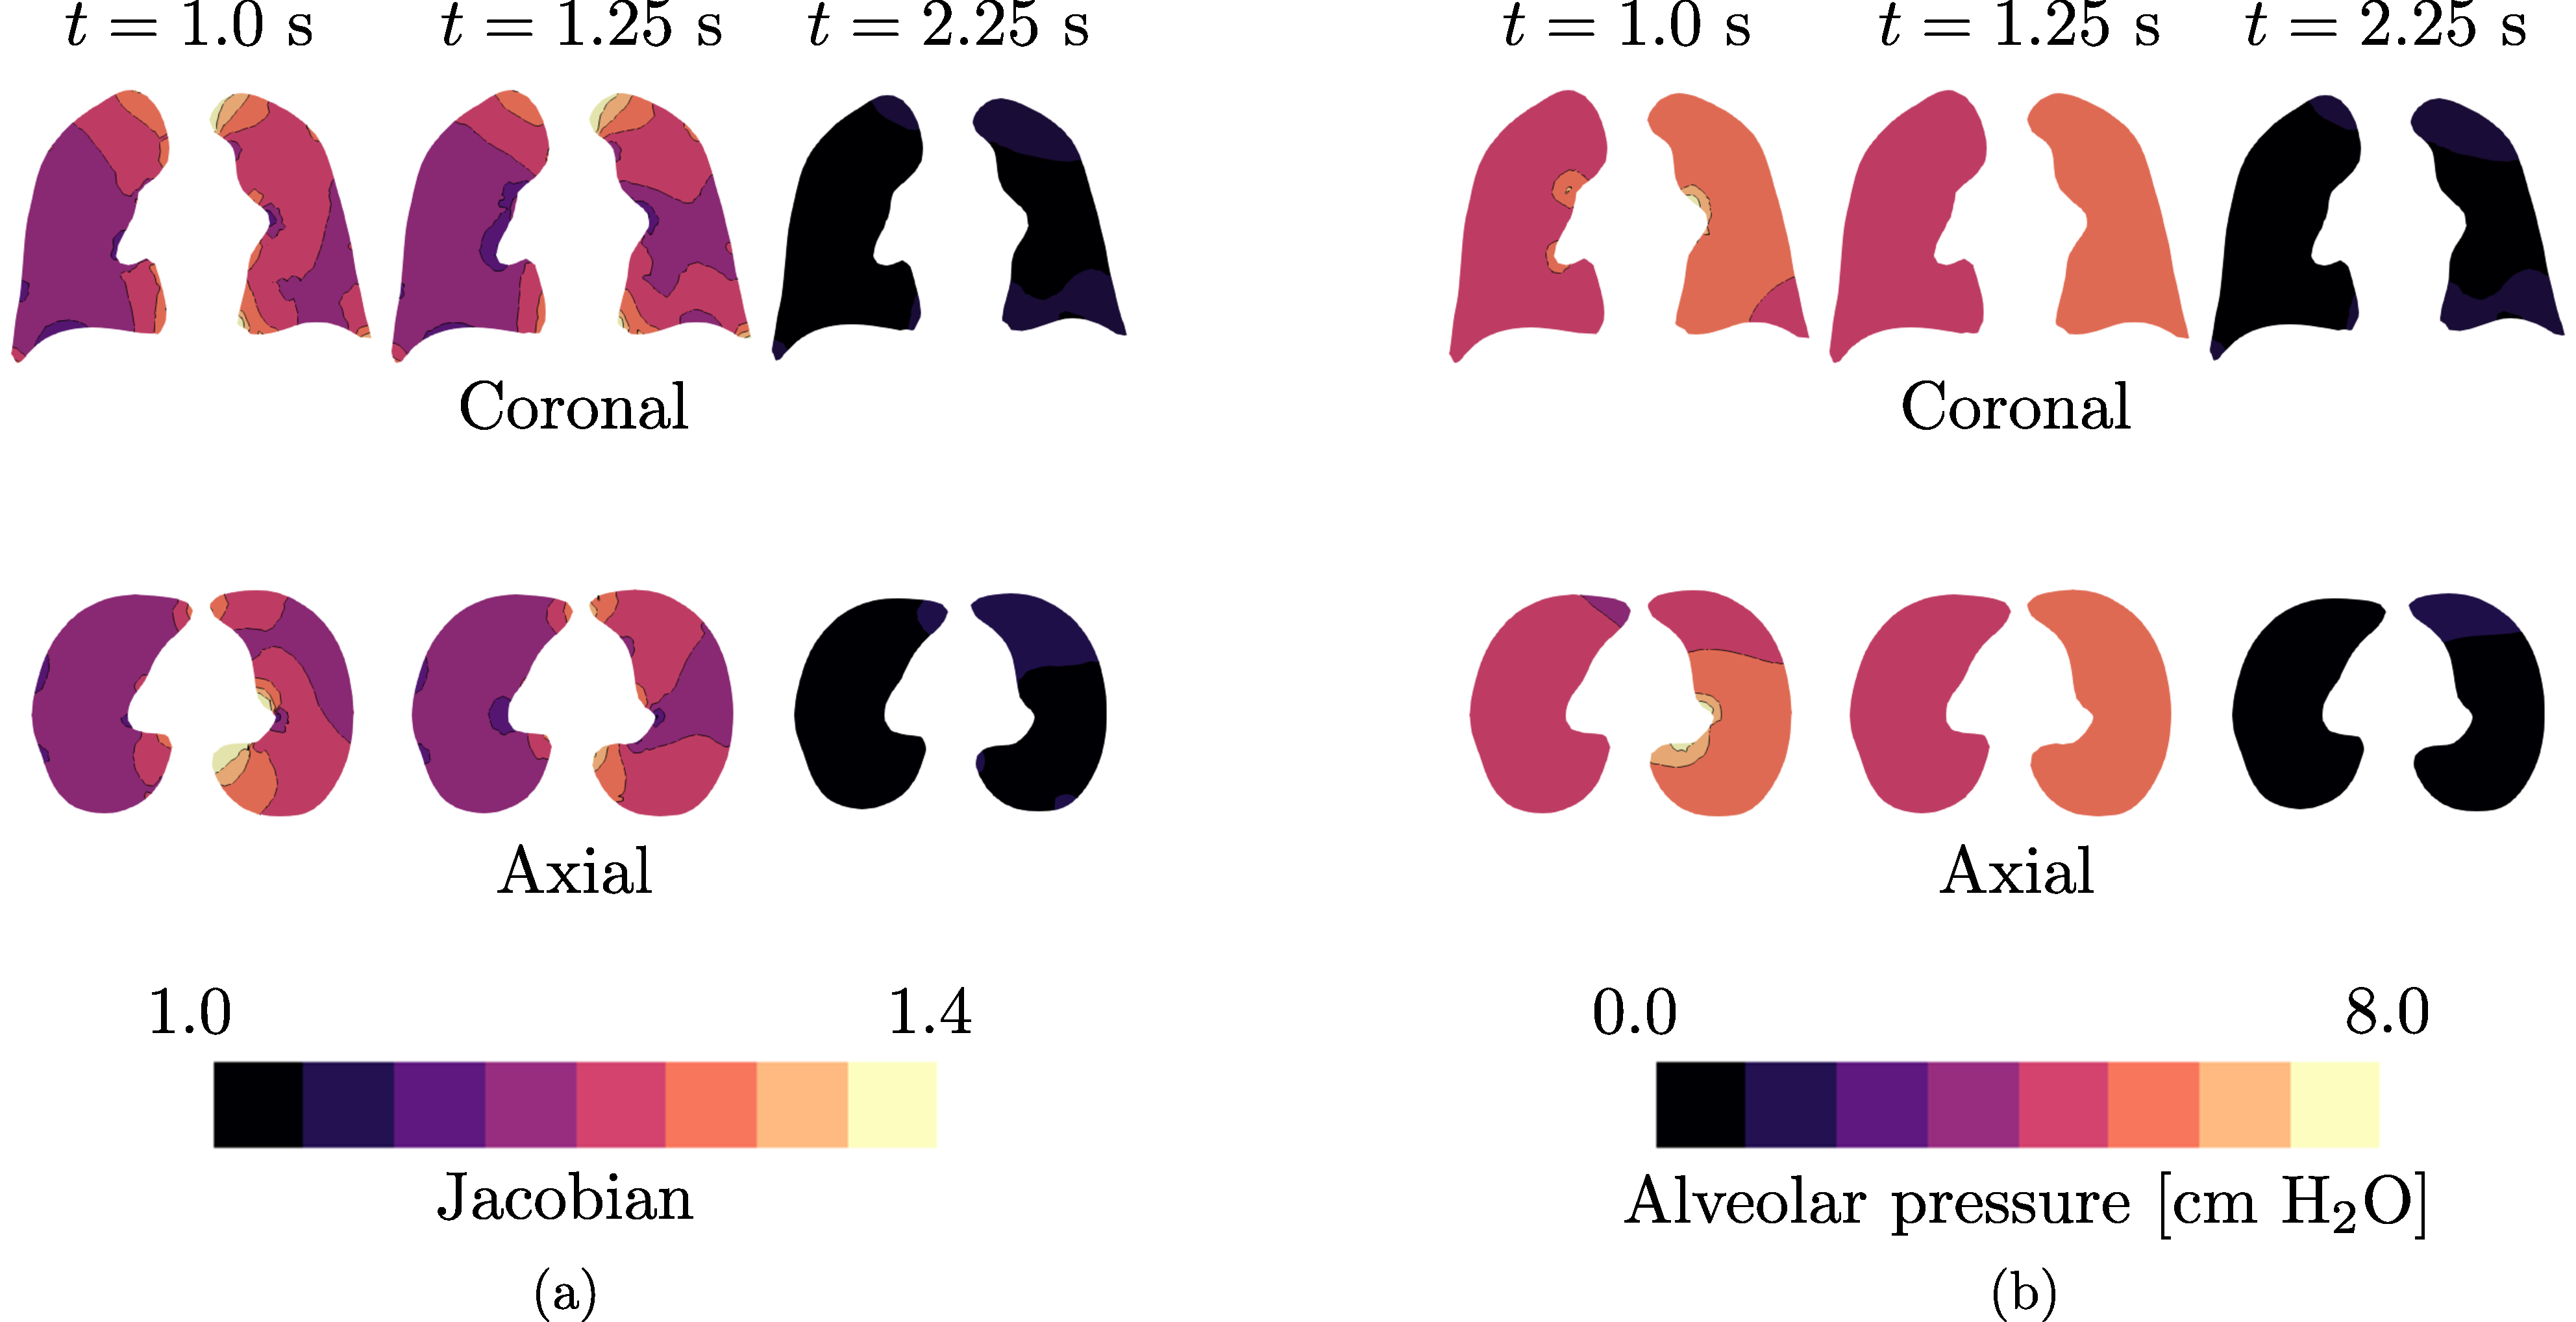
\includegraphics[width=1 \textwidth]{./Figures/jacpres.pdf}
%    \caption[]{\rev{Temporal evolution during one respiratory cycle of volume-controlled
%mechanical ventilation for the case $\mu=10.33$ kPa and $f_0=0.69$: (a) jacobian, and (b) alveolar pressure . Fields are plotted in the current configuration}}
%    \label{fig:fields1}
%    \end{center}
%\end{figure}


%\begin{figure}[h!]
%    \begin{center}
%    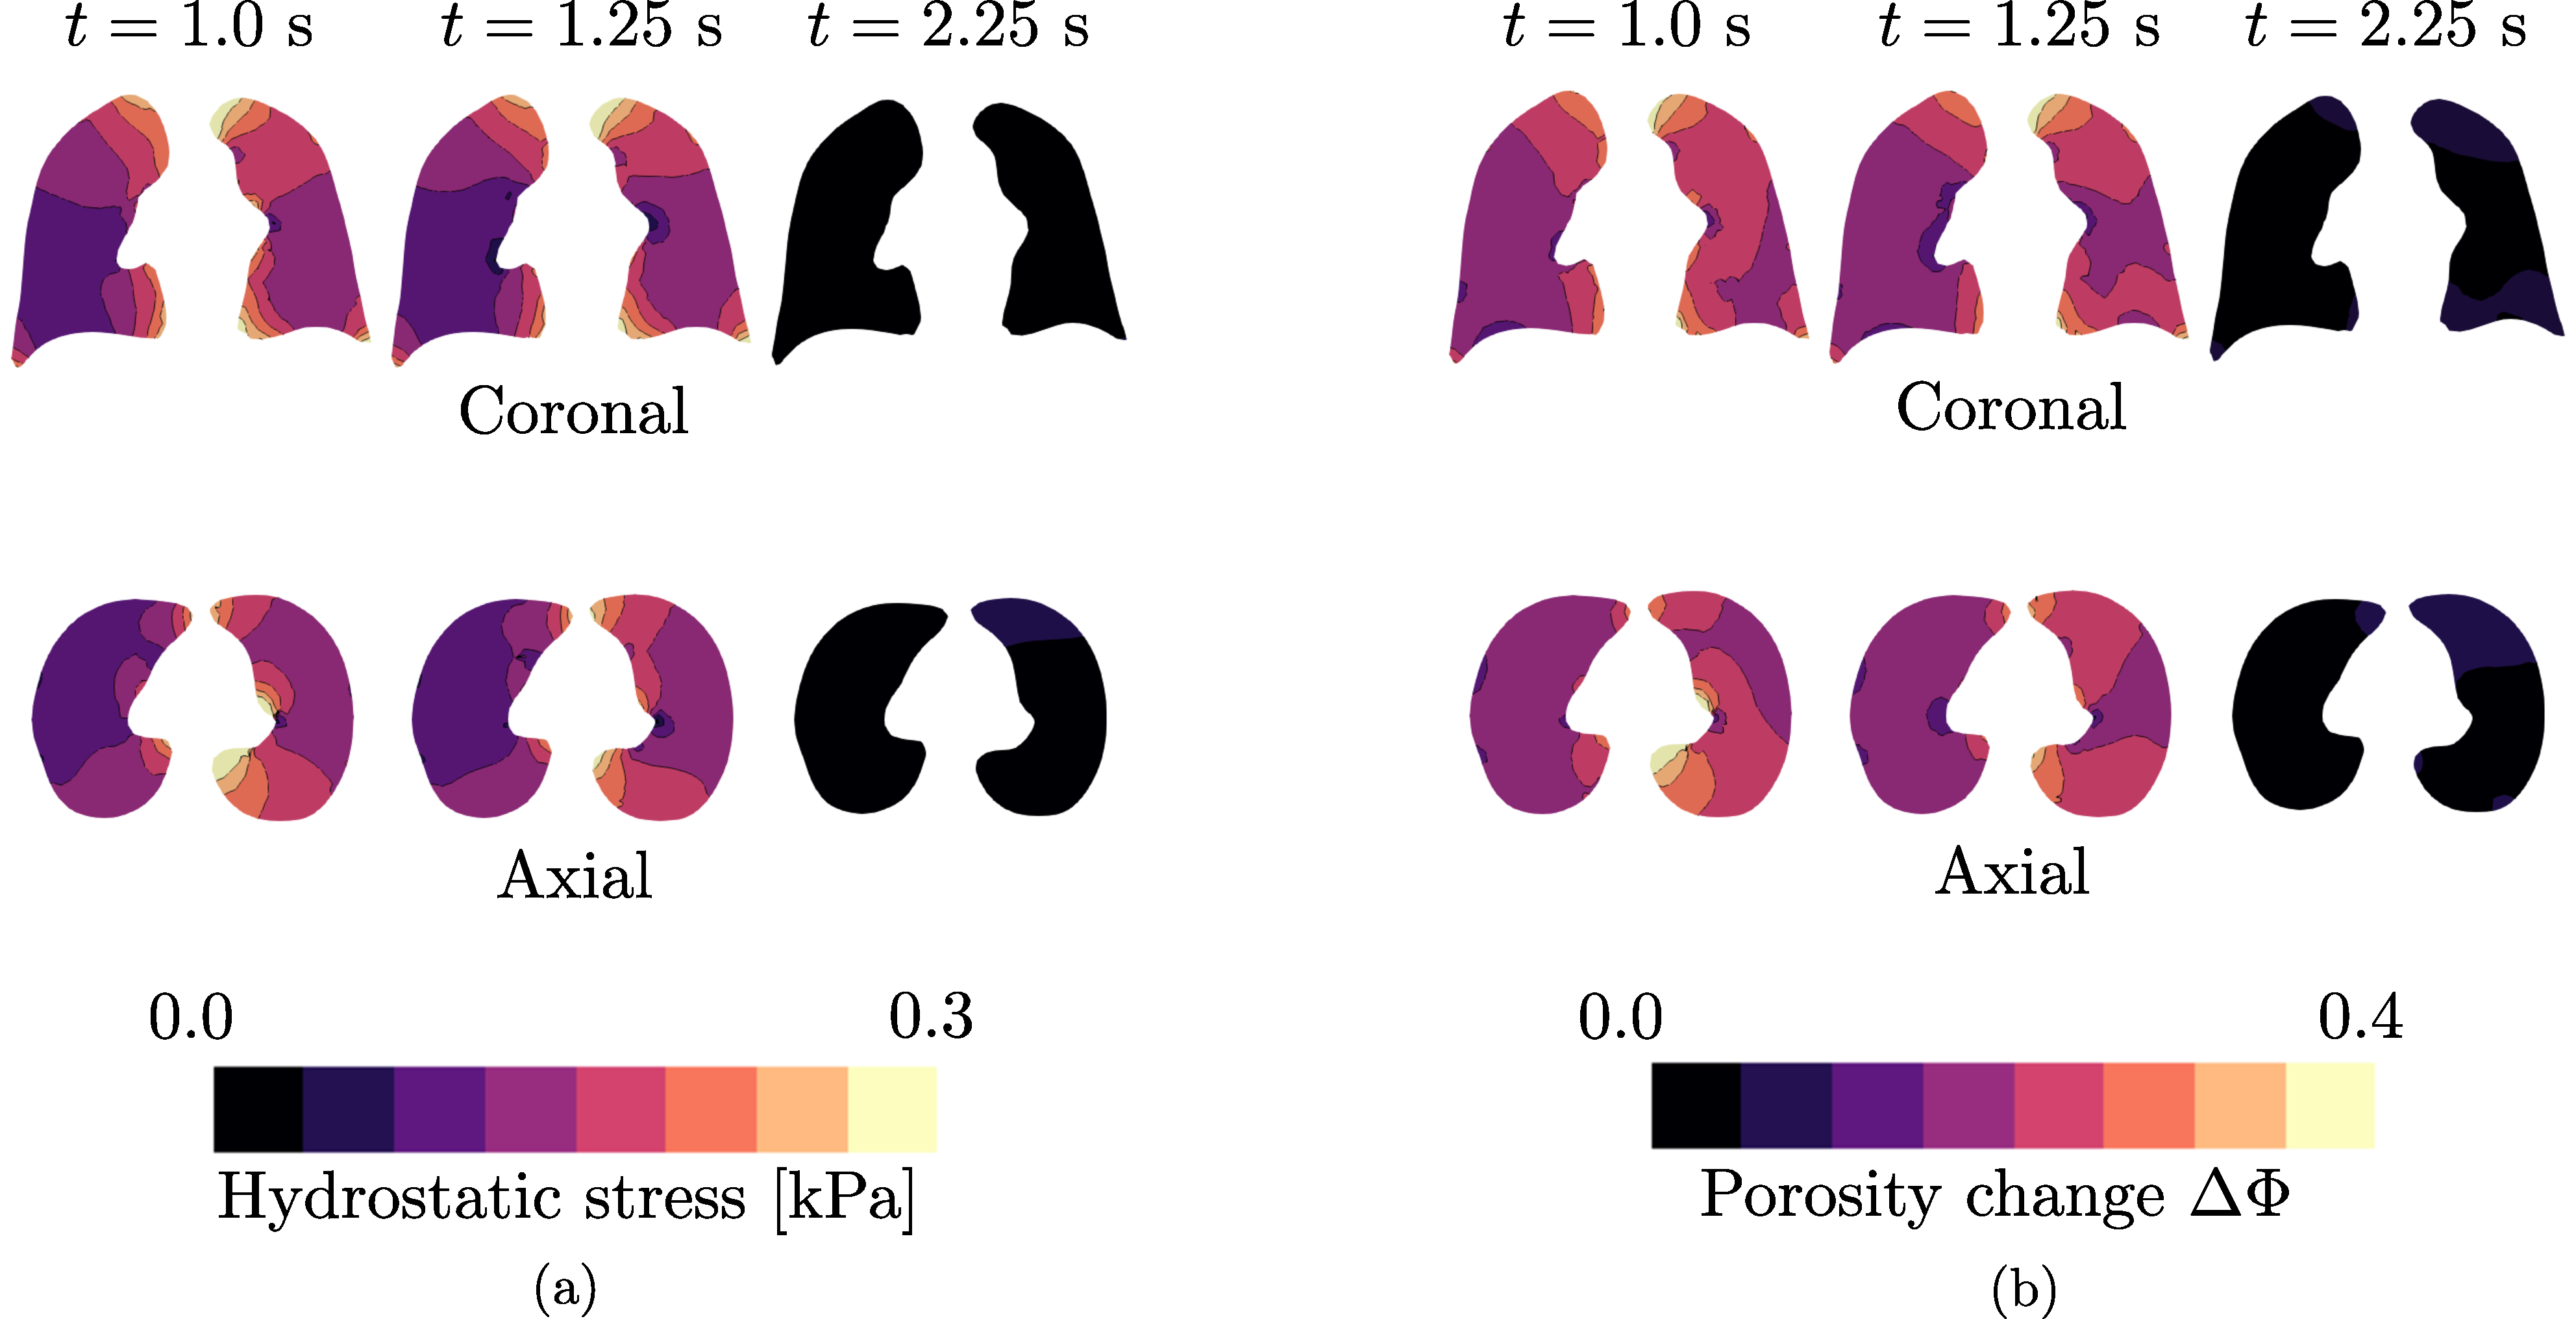
\includegraphics[width=1 \textwidth]{./Figures/hydpor.pdf}
%    \caption[]{\rev{Temporal evolution during one respiratory cycle of volume-controlled
%mechanical ventilation for the case $\mu=10.33$ kPa and $f_0=0.69$: (a) hydrostatic stress, and (b) Material porosity change. Fields are plotted in the current configuration}}
%    \label{fig:fields2}
%    \end{center}
%\end{figure}


%\rev{
%The steady-state was analyzed by constructing the traditional quasi-static pressure-volume curves. For this purpose, the supersyringe technique, that inflates the lung using controlled-volume incremental steps, was used. The curves were constructed using seven inflation steps, where in each one, a constant flow was applied allowing the entry of 100 ml of air in the first 0.3 seconds, in a similar way to the equation \ref{Qpres}. Then, a pause (no flow) of 2 seconds was performed, and the airways pressure was computed according to equation \ref{paw_avg}. Deflation was not considered because, being hyperelastic materials, the difference between the inflation and deflation curves is negligible \cite{berger2016poroelastic,avileshurtado2022whole}. Figures \ref{fig:PV} show the pressure-volume curves obtained. As the PCV and VCV simulations have shown, the parameter $f_0$ seems to have a more significant influence than $\mu$. It is observed that for the same amount of volume, a lower pressure is necessary for lungs with higher porosities, while more rigid lungs need higher pressures.}\\
%\begin{figure}[h!]
%    \begin{center}
%    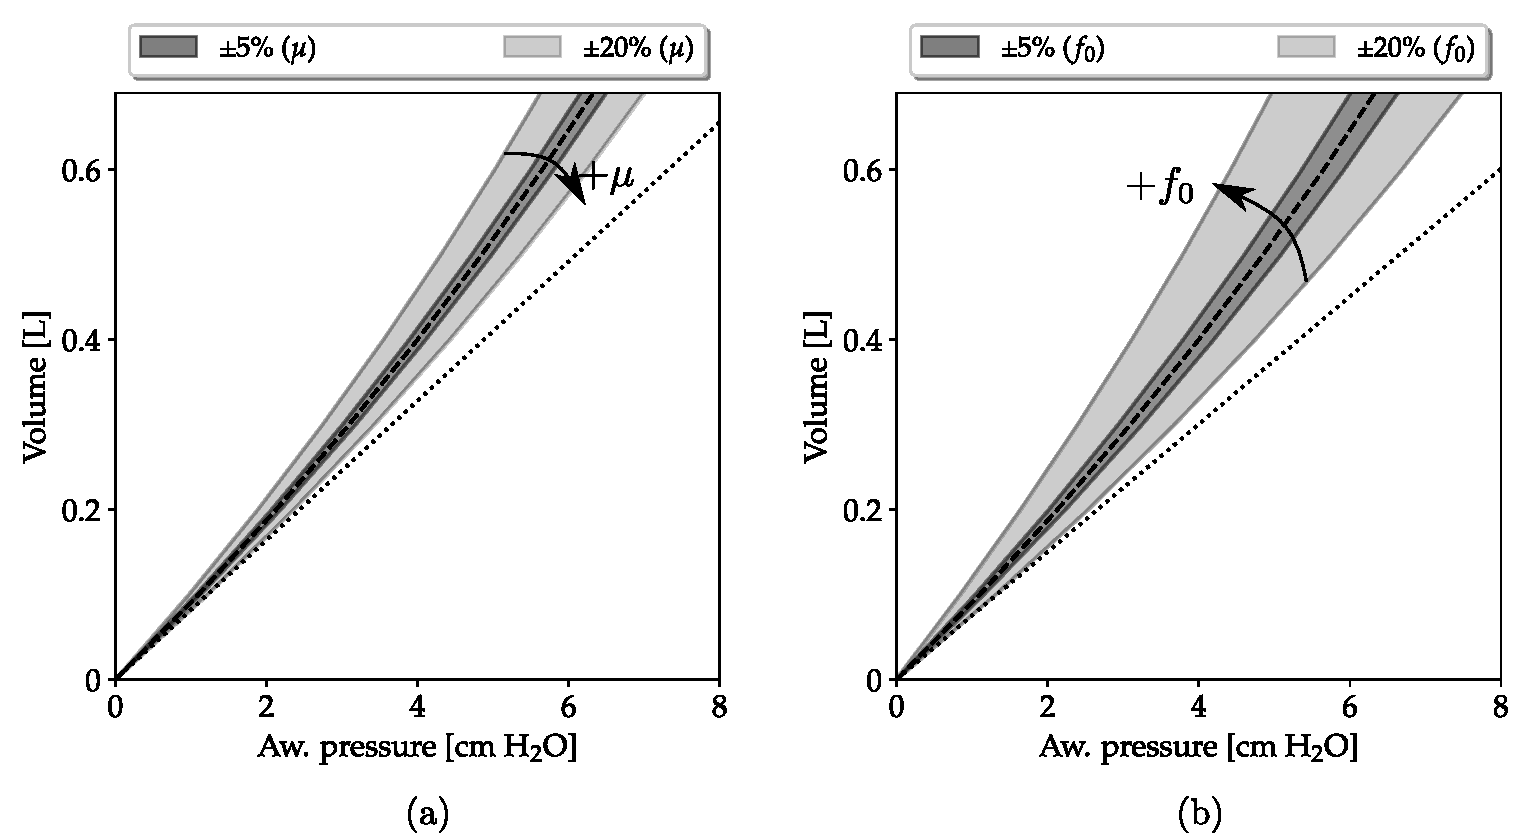
\includegraphics[width=1 \textwidth]{./Figures/SA_super.pdf}
%    \caption[]{\rev{Parameter sensitivity analysis for the quasi-static pressure-volume curves: a) variations in the alveolar-wall elasticity, and b) variations in the initial tissue porosity.}}
%    \label{fig:PV}
%    \end{center}
%\end{figure}








\pagebreak
%%%%%%%%%%%%%%%%%%%%%%%%%%%% DISCUSSION %%%%%%%%%%%%%%%%%%%%%%%%%%%%%%%%%%
\section{Discussion} \label{sec:discussion}

In this work, we present a multiscale model of lung mechanics where alveolar microstructural parameters govern the organ-level mechanical response. Previous continuum models for the estimation of the multiscale lung response were based on a nested dynamic multiscale approach \cite{wiechert2010nested,WallEtal2010}. This technique considers a two-scale deformation-driven homogenization framework, where the fine-scale problem is constructed from an idealized geometry of an alveolar ensemble and is solved using non-linear finite-element analysis. This approach, also known as direct numerical simulation, involves high computational demands as the fine-scale problem requires the solution of a non-linear problem with several thousands of degrees of freedom. From this perspective, the framework proposed in this work offers the advantage of being computationally efficient, as the TKD micromechanical model that informs the tissue level can be five orders of magnitude faster than direct numerical simulations while delivering a similar mechanical response \cite{concha2020upscaling}. This advantage enables the analysis of large-scale problems in reasonable computing times, effectively delivering multiscale predictions of deformation, alveolar pressure, stresses, and porosity fields on complex anatomical geometries that may require a large number of elements in their discretization, see Figures \ref{fig:jac-press-fields} and \ref{fig:hyd-por-field}.\\

Another distinctive feature of our multiscale lung model is its poromechanical foundation, which directly accounts for the air-tissue interaction not captured by traditional deformation-driven lung models. In effect, lung tissue is a highly porous material everywhere in the lung \cite{SarabiaEtal2021}, where air pressurizes the alveolar cavity inducing stresses and strains in the alveolar walls \cite{AlvarezEtal2021}. This tight interaction makes it necessary to couple the alveolar pressure with the tissue deformation \cite{SarabiaEtal2019}. We remark that previous contributions that have addressed lung mechanics using continuum poromechanical formulations consider phenomenological constitutive models for the tissue response \cite{berger2016poroelastic,PatteEtal2022,kowalczyk1993mechanical,avileshurtado2022whole}. These models share the limitation that the constitutive parameters are determined from experimental data obtained from lung tissue samples, and thus they do not directly connect microstructural features to the tissue response. To the best of our knowledge, the present work constitutes one of the first multiscale poromechanical models of the lung informed by alveolar structure and capable of predicting clinically-relevant respiratory mechanics parameters.\\ 

% mech ventilation parameters
Airway pressure, flow, and lung volume are key respiratory signals in intensive care medicine, as they inform doctors in the clinical management of patients connected to mechanical ventilation \cite{Hess2014}. Our multiscale lung model could predict these signals for the two modes of mechanical ventilation studied, PCV and VCV, see Figures \ref{fig:pcv-resp-mechanics} and \ref{fig:vcv-resp-mechanics}, respectively. Remarkably, these signals agree with those observed in ventilated patients, see \cite{LucangeloEtal2005} for a review of respiratory mechanics signals. In the case of PCV, our model predicts flow spikes in response to pressure changes, followed by exponential decay toward zero. This translates into lung volume signals that exponentially increase and decrease, see Figure \ref{fig:pcv-resp-mechanics}. For the VCV mode, lung volume linearly responds to a constant flow, followed by an inspiratory pause where a pressure plateau is reached, see Figure \ref{fig:vcv-resp-mechanics}. After this pause, airway pressure drops to zero, creating a rapid spike followed by a decelerating flow response and an exponential decay in lung volume, which is typically observed in mechanically-ventilated patients \cite{ball2015modes}. Interestingly, when introducing variations in the microstructural parameters, we observe significant changes in the respiratory waveforms that can be related to clinical and experimental observations. For example, in patients under VCV, a decrease in the respiratory-system compliance results in larger peak amplitudes in flow and shorter time scales for the flow and volume during the exponentially-decaying expiratory phase, see \cite{LucangeloEtal2005}. Notably, these waveform changes are recovered by our simulations when the global compliance is reduced due to an increase in alveolar-wall elasticity or a decrease in the initial alveolar porosity, see Figure \ref{fig:vcv-resp-mechanics}. Thus, we confirm that the proposed multiscale lung model can capture dynamic features of lung mechanics observed in human lungs.\\  

Throughout this work, we have shown that the development of a multiscale lung model where the unit cell is constructed upon key parameters that describe the alveolar structure can relate changes in the organ-level function with variations in the microstructure, see Figure \ref{fig:compliance-relations}. While a continuous relation between respiratory compliance and parameters such as alveolar-wall elasticity or alveolar porosity is virtually impossible to achieve in an experimental setting, several investigations have established the connection between alveolar structure changes and their impact on lung function. Studies in normal and fibrotic human lungs have determined Young's modulus of alveolar tissue using atomic-force microscopy \cite{booth2012acellular}, which results from enhanced collagen deposition \cite{snijder2019pulmonary,hinz2012mechanical}. Results show that alveolar-wall elasticity in fibrotic lungs can be $8.4 \times$ greater than that found in normal human lungs. At the same time, respiratory compliance in patients with idiopathic lung fibrosis reduces to 44\% of the value predicted for a normal subject \cite{PlantierEtal2018}. These findings confirm that stiffening of the alveolar wall is associated with significant decreases in the compliance of the respiratory system, a trend that is captured by our sensitivity analysis, see Figure \ref{fig:compliance-relations}(a). These multiscale relationships have also been confirmed in animal models of bleomycin-induced pulmonary fibrosis \cite{DolhnikoffEtal1999}. Another way of assessing the multiscale structure-function relation in the lung is to consider animal studies of pulmonary emphysema. \citet{Parameswaran2009} studied the mechanics and microstructure of normal and emphysematous rat lungs treated with porcine pancreatic elastase using micro-computed tomography. Lung function tests revealed an increase of 37\% in the average dynamic compliance in the emphysema group when compared to the normal group.\footnote{In \cite{Parameswaran2009}, mechanical function is assessed in terms of average dynamic elastance, which can be transformed to compliance by taking its reciprocal value.} Concurrently, the morphological image-based analysis revealed differences of up to $16\times$ in the alveolar airspace volume in emphysematous lungs when compared to normal ones. Noting that porosity directly relates to alveolar airspace volume, these results confirm that increases in alveolar porosity are associated with higher compliance values, a trend recovered by Figure \ref{fig:compliance-relations}(b). Given that compliance measures relative changes in lung volume and airway pressure, the increase of alveolar-wall elasticity is expected to stiffen the lung volume response, as shown in Figure \ref{fig:PV-curves}(a). Analogously, increases in alveolar porosity translate into a softer lung volume response that is readily seen in Figure \ref{fig:PV-curves}(b).\\








%\rev{The impact of microstructural parameters on mechanical ventilation signals, compliance, and pressure-volume curves was analyzed. Remarkably, from a physiological point of view, the variation of these parameters can be related to fatal diseases linked to alterations of the extracellular matrix, such as idiopathic pulmonary fibrosis and emphysema. For example, one of the hallmarks of fibrotic pulmonary tissue is the increase of tissue stiffness due to the enhanced collagen deposition and the remodeling of the ECM \cite{snijder2019pulmonary,hinz2012mechanical,booth2012acellular}. These features are mimicked in our model by increasing the alveolar-wall elasticity. As the volume curves of Figures \ref{fig:PCV}  and  \ref{fig:VCV} shows, the increase of this parameter restricts lung expansion and facilitates contraction during the expiratory phase, resulting in less compliant lungs (see Figure \ref{fig:compliance}), as would be qualitatively expected in fibrotic lungs \cite{nho2022biomechanical}. Also, experiments in fibrotic animal lungs showed marked shifts downward and to the right for the quasi-static pressure-volume curves as a consequence of stiffness tissue \cite{ask2008comparison}, which is also captured by the curves obtained by the supersyringe method, as Figure \ref{fig:PV}a) shows. In the case of emphysema, the destruction of the alveolar-wall and the abnormal enlargement of the air spaces  are typical pathological conditions \cite{snider1985definition,american1995definitions}. These pathologies  can be represented by an increase in the porosity of our model. Indeed, as Figure \ref{fig:PCV} shows, as $f_0$ increases, the lung is hyperinflated and the time constant increases, trapping small volumes of air at the end of expiration. An increase in the time constant and the entrapment of small volumes of air is also predicted in the VCV simulations, as shown in Figure \ref{fig:VCV}. We remark that this behavior is qualitatively similar to that of emphysematous lungs because of the loss of elastic recoil resulting from alveolar destruction \cite{macklem1973pathophysiology,christie1934elastic}. The increase in static compliance expected in an emphysematous lung \cite{papandrinopoulou2012lung} is also captured, as shown by the increase in the slope of pressure-volume curves in Figure \ref{fig:PV}b). Although our model can represent typical features observed in fibrotic or emphysematous patients, values of $\mu$ and $f_0$ representative of human lung diseases could be outside the range considered in this study. The range $\pm$20\% was chosen based on the stability of our model since values outside this range caused convergence problems, which constitutes a limitation of the study, as discussed later.} \\








% multiscale structure-function relationships: connection between alveolar elasticity and porosity with lung compliance

%\cite{Parameswaran2009} shows how rats with emphysema reduce their elastance (i.e., increase their compliance) while increasing porosity (volume fraction?)\\ 

%\cite{DolhnikoffEtal1999} shows how bleomycin-induced fibrosis in rat lungs increases elastance at the organ level and increases collagen (stiffens).\\






%We remark that respiratory mechanics signals have been predicted by traditional single-compartment models in respiratory physiology \cite{Bates2009}. However, it is worth noting that these lump models are highly phenomenological.\\ 

%Our multiscale model can predict from microscopic features, the temporal evolution of macroscopic variables such as mechanical ventilation signals pressure, flow, and volume for the PCV and VCV modes, as shown in Figures \ref{fig:PCV} and \ref{fig:VCV}, respectively. The predicted signals agree with real patients connected to a mechanical ventilator. For PCV simulation, the prescribed square pressure waveform induces a peak flow followed by an exponential decay of flow until the end of inspiration, where the maximum volume is reached. Then, a negative peak flow is reached and also is followed by an exponential decay. In the case of VCV mode, due to the inflow, the peak inspiratory pressure is reached at the end of inspiration, and then, during the pause phase, the well-known plateau pressure \cite{ball2015modes} is recovered. As expected, the prescribed pressure induces a reduction in volume during the expiration. 

%We note that compartment models have previously been proposed to predict mechanical ventilation signals, in which the respiratory system is represented as an interconnected network of elastic elements and resistive conduits \cite{Maury2013,arunachalam2020patient}. However, this  (macroscopic) engineering system approach \cite{Bates2009} does not allow alveolar microstructure to be related to organ response. Also, more complex fractal lumped  models \cite{roth2017comprehensive} that represent the airways' geometry have been proposed. For example, volume-controlled mechanical ventilation was simulated by \citet{roth2017comprehensive}, recovering a peak inspiratory pressure close to 7 cm H$_2$O, a value in line with our predictions. However, although fractal lumped models allow predicting the pressure distribution, by construction, they do not respect the kinematics, not being possible to properly couple the airflow and the alveolar tissue deformation \cite{berger2016poroelastic}.    \\

%\rev{The relationship between the relevant clinical parameter respiratory system compliance and the microstructural parameters was analyzed, see Figure \ref{fig:compliance}. Interestingly, the curves show a non-linear behavior, with a more significant curvature for the case of porosity. A strong dependence on the micromechanical parameters is observed, with both parameters having opposite effects on compliance. For example, while the variation +20\% in the alveolar-wall elasticity induces a reduction in the compliance value up to 85 ml/cm H$_2$O, by increasing the porosity by the same percentage, the compliance increases up to 112 ml/cm H$_2$O. These values are comparable with those of our previous contribution \cite{avileshurtado2022whole}, where we reported values between 15 and 123 ml/cm H$_2$O using different phenomenological constitutive  models. As we note, the compliance values predicted by our multiscale model fall within this range. However, the mechanical response of extremely rigid or compliant phenomenological models cannot be represented in the $\pm 20\%$ range. We remark that, although respiratory system compliance is a clinically relevant parameter, it corresponds to a global estimate of lung deformability during respiration, not providing spatial information on physical quantities. In order to achieve a local understanding, the temporal evolution of the alveolar pressure field and the porosity change (Figure \ref{fig:fields}) was studied for the base case ($\mu=10.33$ kPa, $f_0=0.69 $). The Material porosity change refers to the current porous (air) volume change to the initial volume (tissue and air); and then from a clinical perspective, $\Delta \Phi$ represents the change in gas fraction and regional ventilation. In addition, it should be noted that, due to the tissue incompressibility condition (equation \ref{eq:incomp}), we have that $\Delta \Phi= (d\Omega_x-d\Omega_X )/d\Omega_X$, that is, from a mechanical perspective, the porosity change is equivalent to the volumetric strain. The evolution of this volumetric measure shows a heterogeneous distribution during the VCV cycle, with the apical zone presenting the highest levels of deformation (see the coronal slides Figure \ref{fig:fields}b)). In contrast, a more homogeneous distribution is observed for alveolar pressure; for example, see the axial view at $t_2$ of Figure \ref{fig:fields}a). These observations are consistent with the results presented by \citet{roth2017comprehensive}, who reported more uniform distributions for the pressure field than the volumetric strains. However, the volumetric strains reported in their study present higher magnitudes than our predictions, even though both studies considered similar air tidal volumes. We attribute these differences to the construction of both models since while their study considers a discrete system of alveolar units, we have considered a homogenized continuous medium that, as we have mentioned, connects deformation with regional ventilation. As a consequence, the tissue interaction in our continuum approach results in a stiffer response than fractal models, but with values in the expected range for protective mechanical ventilation \cite{hurtado2020progression}.}\\



The work presented in this contribution offers many opportunities for further improvement. First, we note that only the hyperelastic response of lung tissue was addressed in the model formulation. Alveoli are lined by a thin layer of surfactant, a fluid that exerts surface tension on the alveolar walls \cite{bachofen2001alveolar}. Surface tension on alveolar walls is one of the main responsible for the hysteretic behavior of lungs and cannot be adequately represented by purely elastic constitutive models \cite{QuirosEtal2022}. Future extensions may consider this inelastic contribution by enhancing the current TKD formulation to incorporate existing surfactant models that are based on alveolar surface changes \citet{OtisEtal1994,saad2010dynamic}. Second, for simplicity, we considered an incompressible Neo-Hookean model for the alveolar-wall mechanics. Such a constitutive law does not capture the increase of tangent elastic modulus as the walls deform, mainly attributed to the interaction between collagen and elastin fibers \cite{PerlmanAndWu2014,mead1961mechanical,SukiEtAl2011}. This stiffening effect can be incorporated into the TKD model by considering alternative constitutive relations for the structural elements that compose the TKD \cite{KimmelBudiansky1990}. Finally, our simulations assumed a homogeneous spatial distribution of microstructural parameters. However, spatial variability in tissue ventilation, represented by porosity, is typically observed in lungs under respiratory failure, which is the most frequent condition for which mechanical ventilation is indicated \cite{hurtado2020progression}. Future versions of our multiscale lung model should focus on personalizing lung simulations based on available patient data, which can be achieved using inverse analysis on medical images \cite{PatteEtal2022b}.

%Recently, \citet{maghsoudi2021developing} have shown by inverse finite element analysis that predictions of the displacement field using a model with heterogeneous parameters are better matched than a homogeneous model. 




 

%normal alveoli are lined by a thin continuous fluid that exerts surface forces on the alveolar tissue, which are dynamically modulated by the presence of pulmonary surfactant, leading to hysterical behavior of the lung \cite{bachofen2001alveolar,saad2010dynamic}. 

%This hysterical behavior can be incorporated into the TKD model by quantifying the area change and using surface tension models such as the limited-adsorption model proposed by \citet{OtisEtal1994} or the compression-relaxation model proposed by \citet{saad2010dynamic}. 

%We note that while surface tension has been incorporated into micromechanical models \cite{KimmelBudiansky1990,denny2000viscoelastic,wiechert2009modeling}, predictive poro-inelastic model of the whole lung have not been proposed \cite{concha2020upscaling}. 

%Second, in this work, the mechanical behavior of the alveolar-wall was represented as a Neo-Hookean material, a simple constitutive model that does not allow stiffening to be represented. Experimental studies have reported a strain stiffening of the alveolar-wall \cite{PerlmanAndWu2014}, mainly attributed to the interaction between collagen and elastin fibers \cite{mead1961mechanical, SukiEtAl2011}. Indeed, while the elastin fibers support tension at low deformation, collagen progressively becomes more critical in larger volumes, increasing the general stress of the tissue and giving rise to the asymptotic shape of the pressure-volume curves \cite{suki2011lung}. 

%The interaction between the structural fibers of the alveolar-wall should be considered in future developments. 

%In this context, we believe that the convergence problems presented are due to the absence of stiffening, so a micromechanical model that includes the interaction between collagen and elastin fibers could improve the numerical stability of our model. 

%Finally, this work uses homogeneous parameters throughout the lung, disregarding their spatial variability. Considering spatial variability is essential for analyzing lungs with acute respiratory distress syndrome, which presents heterogeneous distributions of parameters such as porosity, with marked differences between normal tissues and diseases \cite{gattinoni2001has}. Recently, \citet{maghsoudi2021developing} have shown by inverse finite element analysis that predictions of the displacement field using a model with heterogeneous parameters are better matched than a homogeneous model. Future developments should focus on personalizing lung computational models for each patient, which can be done by solving an inverse problem from clinical data and images \cite{PatteEtal2022} .\\


%represented the mechanical behavior of the whole lung through poroelastic models; however, their phenomenological foundation does not allow connecting the tissue with microstructural features like its open foam polyhedral geometry \cite{concha2020upscaling}.\\

%\rev{In this work, a multiscale model of finite deformation lung poroelasticity has been introduced, suitable for simulating mechanical ventilation considering the influence of microstructural parameters on the whole-lung response. To this end, we construct a non-linear tissue constitutive model informed by the alveolar level (fine-scale), and then, using a multiscale poromechanical framework, we perform an upscaling to the whole lung level (coarse-scale). Multiscale attempts to predict the finite-deformation mechanical response of the lung have been previously performed by \citet{wiechert2010nested}. They propose a nested dynamic multiscale approach, where the coarse and fine scales are fully coupled in a deformation-driven procedure and are simultaneously resolved by finite element analysis. This approach is computationally expensive since the fine-scale problem involves solving non-linear systems with thousands of DOFs (degrees of freedom). Consequently, this DNS multiscale approach is limited to regular geometries, such as cubes or lung tissue strips and idealized loads, as a proof of concept. In contrast, our computational implementation is more efficient in numerical terms because, based on geometry and periodicity considerations, the fine-scale problem requires the solution of an optimization problem that only has 3 DOFs, being our model suitable for whole organ simulations \cite{concha2020upscaling}. Another advantage is the fact that, as we consider a poromechanical framework, by construction, the parenchyma response is not only driven by deformation but also by pressure, allowing it to represent the interaction between air and alveolar tissue. Indeed, the lung parenchyma is a porous material where the air pressurizes the alveolar walls, making it necessary to couple the alveolar pressure with the tissue deformation \cite{SarabiaEtal2021}. We remark that prior works \cite{berger2016poroelastic,PatteEtal2022,kowalczyk1993mechanical,avileshurtado2022whole} have represented the mechanical behavior of the whole lung through poroelastic models; however, their phenomenological foundation does not allow connecting the tissue with microstructural features like its open foam polyhedral geometry \cite{concha2020upscaling}.}\\


%\rev{Our multiscale model can predict from microscopic features, the temporal evolution of macroscopic variables such as mechanical ventilation signals pressure, flow, and volume for the PCV and VCV modes, as shown in Figures \ref{fig:PCV} and \ref{fig:VCV}, respectively. The predicted signals agree with real patients connected to a mechanical ventilator. For PCV simulation, the prescribed square pressure waveform induces a peak flow followed by an exponential decay of flow until the end of inspiration, where the maximum volume is reached. Then, a negative peak flow is reached and also is followed by an exponential decay. In the case of VCV mode, due to the inflow, the peak inspiratory pressure is reached at the end of inspiration, and then, during the pause phase, the well-known plateau pressure \cite{ball2015modes} is recovered. As expected, the prescribed pressure induces a reduction in volume during the expiration. We note that compartment models have previously been proposed to predict mechanical ventilation signals, in which the respiratory system is represented as an interconnected network of elastic elements and resistive conduits \cite{Maury2013,arunachalam2020patient}. However, this  (macroscopic) engineering system approach \cite{Bates2009} does not allow alveolar microstructure to be related to organ response. Also, more complex fractal lumped  models \cite{roth2017comprehensive} that represent the airways' geometry have been proposed. For example, volume-controlled mechanical ventilation was simulated by \citet{roth2017comprehensive}, recovering a peak inspiratory pressure close to 7 cm H$_2$O, a value in line with our predictions. However, although fractal lumped models allow predicting the pressure distribution, by construction, they do not respect the kinematics, not being possible to properly couple the airflow and the alveolar tissue deformation \cite{berger2016poroelastic}. } \\


%\rev{The relationship between the relevant clinical parameter respiratory system compliance and the microstructural parameters was analyzed, see Figure \ref{fig:compliance}. Interestingly, the curves show a non-linear behavior, with a more significant curvature for the case of porosity. A strong dependence on the micromechanical parameters is observed, with both parameters having opposite effects on compliance. For example, while the variation +20\% in the alveolar-wall elasticity induces a reduction in the compliance value up to 85 ml/cm H$_2$O, by increasing the porosity by the same percentage, the compliance increases up to 112 ml/cm H$_2$O. These values are comparable with those of our previous contribution \cite{avileshurtado2022whole}, where we reported values between 15 and 123 ml/cm H$_2$O using different phenomenological constitutive  models. As we note, the compliance values predicted by our multiscale model fall within this range. However, the mechanical response of extremely rigid or compliant phenomenological models cannot be represented in the $\pm 20\%$ range. We remark that, although respiratory system compliance is a clinically relevant parameter, it corresponds to a global estimate of lung deformability during respiration, not providing spatial information on physical quantities. In order to achieve a local understanding, the temporal evolution of the alveolar pressure field and the porosity change (Figure \ref{fig:fields}) was studied for the base case ($\mu=10.33$ kPa, $f_0=0.69 $). The Material porosity change refers to the current porous (air) volume change to the initial volume (tissue and air); and then from a clinical perspective, $\Delta \Phi$ represents the change in gas fraction and regional ventilation. In addition, it should be noted that, due to the tissue incompressibility condition (equation \ref{eq:incomp}), we have that $\Delta \Phi= (d\Omega_x-d\Omega_X )/d\Omega_X$, that is, from a mechanical perspective, the porosity change is equivalent to the volumetric strain. The evolution of this volumetric measure shows a heterogeneous distribution during the VCV cycle, with the apical zone presenting the highest levels of deformation (see the coronal slides Figure \ref{fig:fields}b)). In contrast, a more homogeneous distribution is observed for alveolar pressure; for example, see the axial view at $t_2$ of Figure \ref{fig:fields}a). These observations are consistent with the results presented by \citet{roth2017comprehensive}, who reported more uniform distributions for the pressure field than the volumetric strains. However, the volumetric strains reported in their study present higher magnitudes than our predictions, even though both studies considered similar air tidal volumes. We attribute these differences to the construction of both models since while their study considers a discrete system of alveolar units, we have considered a homogenized continuous medium that, as we have mentioned, connects deformation with regional ventilation. As a consequence, the tissue interaction in our continuum approach results in a stiffer response than fractal models, but with values in the expected range for protective mechanical ventilation \cite{hurtado2020progression}.}\\

%\rev{The impact of microstructural parameters on mechanical ventilation signals, compliance, and pressure-volume curves was analyzed. Remarkably, from a physiological point of view, the variation of these parameters can be related to fatal diseases linked to alterations of the extracellular matrix, such as idiopathic pulmonary fibrosis and emphysema. For example, one of the hallmarks of fibrotic pulmonary tissue is the increase of tissue stiffness due to the enhanced collagen deposition and the remodeling of the ECM \cite{snijder2019pulmonary,hinz2012mechanical,booth2012acellular}. These features are mimicked in our model by increasing the alveolar-wall elasticity. As the volume curves of Figures \ref{fig:PCV}  and  \ref{fig:VCV} shows, the increase of this parameter restricts lung expansion and facilitates contraction during the expiratory phase, resulting in less compliant lungs (see Figure \ref{fig:compliance}), as would be qualitatively expected in fibrotic lungs \cite{nho2022biomechanical}. Also, experiments in fibrotic animal lungs showed marked shifts downward and to the right for the quasi-static pressure-volume curves as a consequence of stiffness tissue \cite{ask2008comparison}, which is also captured by the curves obtained by the supersyringe method, as Figure \ref{fig:PV}a) shows. In the case of emphysema, the destruction of the alveolar-wall and the abnormal enlargement of the air spaces  are typical pathological conditions \cite{snider1985definition,american1995definitions}. These pathologies  can be represented by an increase in the porosity of our model. Indeed, as Figure \ref{fig:PCV} shows, as $f_0$ increases, the lung is hyperinflated and the time constant increases, trapping small volumes of air at the end of expiration. An increase in the time constant and the entrapment of small volumes of air is also predicted in the VCV simulations, as shown in Figure \ref{fig:VCV}. We remark that this behavior is qualitatively similar to that of emphysematous lungs because of the loss of elastic recoil resulting from alveolar destruction \cite{macklem1973pathophysiology,christie1934elastic}. The increase in static compliance expected in an emphysematous lung \cite{papandrinopoulou2012lung} is also captured, as shown by the increase in the slope of pressure-volume curves in Figure \ref{fig:PV}b). Although our model can represent typical features observed in fibrotic or emphysematous patients, values of $\mu$ and $f_0$ representative of human lung diseases could be outside the range considered in this study. The range $\pm$20\% was chosen based on the stability of our model since values outside this range caused convergence problems, which constitutes a limitation of the study, as discussed later.} \\

%\rev{This work offers a multiscale connection between the biomechanics of the ECM with macroscopic variables and parameters relevant to respiratory medicine. There are different ways to improve our model, which represent research opportunities. First, normal alveoli are lined by a thin continuous fluid that exerts surface forces on the alveolar tissue, which are dynamically modulated by the presence of pulmonary surfactant, leading to hysterical behavior of the lung \cite{bachofen2001alveolar,saad2010dynamic}. This hysterical behavior can be incorporated into the TKD model by quantifying the area change and using surface tension models such as the limited-adsorption model proposed by \citet{OtisEtal1994} or the compression-relaxation model proposed by \citet{saad2010dynamic}. We note that while surface tension has been incorporated into micromechanical models \cite{KimmelBudiansky1990,denny2000viscoelastic,wiechert2009modeling}, predictive poro-inelastic model of the whole lung have not been proposed \cite{concha2020upscaling}. Second, in this work, the mechanical behavior of the alveolar-wall was represented as a Neo-Hookean material, a simple constitutive model that does not allow stiffening to be represented. Experimental studies have reported a strain stiffening of the alveolar-wall \cite{PerlmanAndWu2014}, mainly attributed to the interaction between collagen and elastin fibers \cite{mead1961mechanical, SukiEtAl2011}. Indeed, while the elastin fibers support tension at low deformation, collagen progressively becomes more critical in larger volumes, increasing the general stress of the tissue and giving rise to the asymptotic shape of the pressure-volume curves \cite{suki2011lung}. The interaction between the structural fibers of the alveolar-wall should be considered in future developments. In this context, we believe that the convergence problems presented are due to the absence of stiffening, so a micromechanical model that includes the interaction between collagen and elastin fibers could improve the numerical stability of our model. Finally, this work uses homogeneous parameters throughout the lung, disregarding their spatial variability. Considering spatial variability is essential for analyzing lungs with acute respiratory distress syndrome, which presents heterogeneous distributions of parameters such as porosity, with marked differences between normal tissues and diseases \cite{gattinoni2001has}. Recently, \citet{maghsoudi2021developing} have shown by inverse finite element analysis that predictions of the displacement field using a model with heterogeneous parameters are better matched than a homogeneous model. Future developments should focus on personalizing lung computational models for each patient, which can be done by solving an inverse problem from clinical data and images \cite{PatteEtal2022} }.\\

\section*{Acknowledgements}
This work was funded by the National Agency for Research and Development (ANID) of Chile through the grant FONDECYT Regular \# 1220465. NA-R acknowledges the support of the graduate fellowship ANID BECAS/DOCTORADO NACIONAL 21212320.


%%%%%%%%%%%%%%%%%%% APPENDIX %%%%%%%%%%%%%%%%%%%%%%%%%%%%%%%
%% The Appendices part is started with the command \appendix;
%% appendix sections are then done as normal sections


%\appendix
%\section{TKD implementation for coarse-scale stress tensor}

%We will define the auxiliary term $\pd{\vec r}{\ten F^c}$. To do that, we use the residual of the potential enery such that:
%\begin{eqnarray*}
%	\pd{\Pi^{eff}}{\vec r} (\vec r^{*}; \ten F^c, p_{alv}^c) =\vec 0 
%\end{eqnarray*}
%
%Now, deriving last equation with respect to $\ten F^c$,
%\begin{eqnarray*}
	%\pddc{\Pi^{eff}}{\vec r}{\vec r} : \pd{\vec r}{\ten F^c} + \pddc{\Pi^{eff}}{\ten F^c}{\vec r} = \ten 0
%\end{eqnarray*}
%Which, in indicial notation leads to
%\begin{equation*}
	%\pddc{\Pi^{eff}}{r_p}{r_m} \pd{r_p}{F_{ij}^c} + \pddc{\Pi^{eff}}{F_{ij}^c}{r_m} = 0_m
%\end{equation*}
%At this point, we define two new variables for simplify notation
%\begin{equation*}
	%K_{pm} = \pddc{\Pi^{eff}}{r_p}{r_m}; \qquad G_{ijm} = \pddc{\Pi^{eff}}{F^c_{ij}}{r_m}
%\end{equation*}
%Now, solving for $\pd{\vec r}{\ten F^c}$, 
%\begin{eqnarray*}
%	\pd{r_p}{F_{ij}^c} = -K^{-1}_{pm} G_{ijm}
%\end{eqnarray*}
%


%Now, we find the expressions for the elasticity tensor in the principal directions. For the sake of notation
%we will just denote it as $\pd{\ten P^c}{\ten F^c}$
%\begin{equation*}
	%\pd{\ten P^c}{\ten F^c} =\frac{1}{V_0} \pd{}{\ten F^c} \left[\pd{\Pi^{eff}}{\vec r} : \pd{\vec r}{\ten F^c} + \pd{\Pi^{eff}}{\ten F^c} \right] 
%\end{equation*}
%Using indicial notation, it becomes
%\begin{equation*}
%	\pd{\ten P^c}{\ten F^c} = \frac{1}{V_0} \pd{}{F_{kl}^c} \left[
	%\pd{\Pi^{eff}}{r_p} \pd{r_p}{F_{ij}^c} + \pd{\Pi^{eff}}{F_{ij}^c} \right] 
%\end{equation*}

%\begin{equation*}
	%V_0 \mathcal C_{ijkl}^c = \left( \pddc{\Pi^{eff}}{r_q}{r_p} \pd{r_q}{F_{kl}^c} + \pddc{\Pi^{eff}}{F_{kl}^c}{r_p} \right) \pd{r_p}{F_{ij}^c} \quad + \quad 
	%\pd{\Pi^{eff}}{r_p} \pddc{r_p}{F_{kl}^c}{F_{ij}^c} \quad + \quad 
	%\left( \pddc{\Pi^{eff}}{r_p}{F_{ij}^c} \pd{r_p}{F_{kl}^c} + \pddc{\Pi^{eff}}{F_{kl}^c} {F_{ij}^c}  \right) 
%\end{equation*}
%
%but using the terms we defined before, we see that the first term in brackets is zero
%\begin{eqnarray*}
	%\pddc{W^c}{r_q}{r_p} \pd{r_q}{F_{kl}^c} + \pddc{W^c}{F_{kl}^c}{r_p} 
%	&=& -K_{qp} K_{qm}^{-1} G_{klm}  + G_{klp} \\
%	&=& -K_{pq} K_{qm}^{-1} G_{klm}  + G_{klp} \\
	%&=& -\delta_{pm} G_{klm} + G_{klp} \\
	%&=& -G_{klp} + G_{klp} \\
	%&=& 0
%\end{eqnarray*}
%while the secnd term is zero because it contains the residual expression evaluated at the solution of the degrees of freedom. So, finally we have
%\begin{equation*}
%	\pd{\ten P^c}{\ten F^c} = \frac{1}{V_0} \left(\pddc{\Pi^{eff}}{r_p}{F_{ij}^c} \pd{r_p}{F_{kl}^c} + \pddc{\Pi^{eff}}{F_{kl}^c} {F_{ij}^c} \right)
%\end{equation*}

%Now, we have to compute another auxiliary term, which is still expressed in principal directions
%\begin{equation}
	%\pd{\ten S^c}{\ten F^c} = \pd{}{\ten F^c} \left( \ten F^{c^{-1}} \ten P^{c} \right)
%\end{equation}
%Using indicial notation, we have that
%\begin{equation}
	%\pd{S_{ij}}{F^c_{kl}} = -F^{c^{-1}}_{i,k} F^{c^{-1}}_{l,q} P^c_{q,j} + F^{c^{-1}}_{i,q} \pd{P^c_{q,j}}{F^c_{k,l}}
%\end{equation}

%So, based on the expression in \cite{Holzapfel}, we finally compute the elasticity tensor for non-diagonal coordinates as:
%\begin{align}
	%\mathbb{C^c} = \sum_{a,b=1}^3 \frac{1}{\lambda_b^c} \pd{S_a^c}{\lambda_b^c} \vec{\hat N}_a \otimes \vec{\hat N}_a \otimes \vec{\hat N}_b \otimes \vec{\hat N}_b + \\
	%
	%\sum\limits_{\substack{a,b=1 \\a \neq b}}^3 \frac{S_b^c - S_a^c}{\lambda_b^{c^2} - \lambda_a^{c^2}} \left( \vec{\hat N}_a \otimes \vec{\hat N}_b \otimes \vec{\hat N}_a \otimes \vec{\hat N}_b + \vec{\hat N}_a \otimes \vec{\hat N}_b \otimes \vec{\hat N}_b \otimes \vec{\hat N}_a \right) \label{eqn:elasticity_tensor}
%\end{align}	










%% References with bibTeX database:
%\section*{References}
\bibliographystyle{elsarticle-harv}
\bibliography{refs_HurtadoConcha2020}


\end{document}



